\documentclass[a4paper]{article}    % define document layout
%\documentclass[draft]{article}     % use draft option in packages
%-----------------------------
% preamble
%-----------------------------
\usepackage[sumlimits,]{amsmath}    % math equations and formulas
\usepackage[utf8]{inputenc}         % use UTF-8 encoding
\usepackage[english]{babel}         % use English language
\usepackage{graphicx}              % insert images
%\usepackage[draft]{graphicx}        % do not render figures
\usepackage{subcaption}             % multiple images in one figure
\usepackage{hyperref}               % hyperlinks
\usepackage{float}                  % floating objects (figures, tables)
\usepackage{geometry}               % page size and margins
\geometry{a4paper, margin=1in}      % margins
\usepackage{ragged2e}               % text alignment
%\usepackage{multirow}               % merge rows in table

\graphicspath{                      % path for figures
    {../figures/} 
    {../figures/mlp/} 
    {../figures/svm/} 
}

%-----------------------------
% body
%-----------------------------
\begin{document}

\begin{figure}
    \centering
    % UNICAMP logo
    \begin{subfigure}{0.45\textwidth}
        \centering
        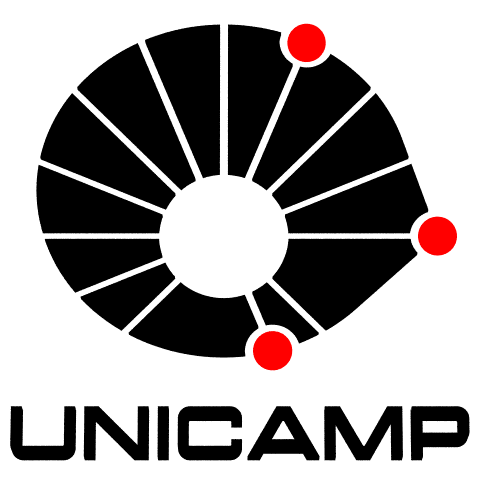
\includegraphics[width=1.5cm]{unicamp}
%        \label{fig:unicamp}
    \end{subfigure}
    \hfill
    % FEEC logo
    \begin{subfigure}{0.45\textwidth}
        \centering
        
\includegraphics[width=1.5cm]{feec}
%        \label{fig:feec}
    \end{subfigure}
\end{figure}

\title{EFC3 - Exercise 3}
\author{Rafael Claro Ito (R.A.: 118430)}
%R.A.: 118430
%ito.rafael@gmail.com
\date{November 2019}
\maketitle
\newpage

%=================================================
\section{Source files}
%=================================================

\paragraph{All code cited and all figures showed here can be found at the following GitHub repository:\\
\url{https://github.com/ito-rafael/IA006C-MachineLearning/tree/master/efc3}\\
In this repository, one can found the following files:\\}

\begin{itemize}
    \item Jupyter Notebook
    \begin{itemize}
        \item \href{https://github.com/ito-rafael/IA006C-MachineLearning/tree/master/efc3/notebooks}{MLP.ipynb}
        \item \href{https://github.com/ito-rafael/IA006C-MachineLearning/blob/master/efc3/notebooks/SVM.ipynb}{SVM.ipynb}
    \end{itemize}
    \item \LaTeX
    \begin{itemize}
        \item \href{https://github.com/ito-rafael/IA006C-MachineLearning/blob/master/efc3/latex/efc3.tex}{efc3.tex}
    \end{itemize}
\end{itemize}

\paragraph{The notebook ``MLP'' implements a multi-layer perceptron network used for binary classification. Here, we use different numbers of neurons, plot the decision regions and also calculate some metrics to evaluate the overall performance.}

\paragraph{The notebook ``SVM'' uses the same dataset and also implements a binary classifier, but it does this using a support vector machine. Here, we plot the decision regions as well, but this time we vary the value of the hyperparameter C and also the value gamma used in a RBF kernel.}

\bigskip

%=================================================
\section{Part I - Error backpropagation}
%=================================================

$ u_1 = 1 \cdot v_{00} + x_1 \cdot v_{10} + x_2 \cdot v_{20} $\\
$ u_2 = 1 \cdot v_{01} + x_1 \cdot v_{11} + x_2 \cdot v_{21} $\\
$ u_3 = 1 \cdot v_{02} + x_1 \cdot v_{12} + x_2 \cdot v_{22} $\\
\vspace{0.1mm}\\
%
$ s_1 = f(u_1) $\\
$ s_2 = f(u_2) $\\
$ s_3 = f(u_3) $\\
\vspace{0.1mm}\\
%
$ y_1 = 1 \cdot w_{00} + s_1 \cdot w_{10} + s_2 \cdot w_{20} + s_3 \cdot w_{30} $\\
$ y_2 = 1 \cdot w_{01} + s_1 \cdot w_{11} + s_2 \cdot w_{21} + s_3 \cdot w_{31} $\\
\vspace{0.1mm}\\
%
$ J = e_1^2 + e_2^2 $\\
\vspace{0.1mm}\\
%
$ \delta_3 = \dfrac{\partial J}{\partial u_3} = \dfrac{\partial [(d_1-y_1)^2+(d_2-y_2)^2]}{\partial u_3} $\\
$ \delta_3 = \dfrac{\partial (d_1-y_1)^2}{\partial u_3} + \dfrac{\partial (d_2-y_2)^2}{\partial u_3} $\\
$ \delta_3 = \dfrac{\partial (d_1-y_1)^2}{\partial (d_1-y_1)} \cdot \dfrac{\partial (d_1-y_1)}{\partial u_3} + \dfrac{\partial (d_2-y_2)^2}{\partial (d_2-y_2)} \cdot \dfrac{\partial (d_2-y_2)}{\partial u_3} $\\
$ \delta_3 = 2(d_1-y_1) \cdot \left(-\dfrac{\partial y_1}{\partial u_3}\right) + 2(d_2-y_2) \cdot \left(-\dfrac{\partial y_2}{\partial u_3}\right) $\\
$ \delta_3 = - 2(d_1-y_1) \cdot \dfrac{\partial y_1}{\partial s_3} \cdot \dfrac{\partial s_3}{\partial u_3} - 2(d_2-y_2) \cdot \dfrac{\partial y_2}{\partial s_3} \cdot \dfrac{\partial s_3}{\partial u_3} $
%$ \delta_3 = - 2(d_1-y_1) \cdot \dfrac{\partial (1 \cdot w_{00} + s_1 \cdot w_{10} + s_2 \cdot w_{20} + s_3 \cdot w_{30})}{\partial s_3} \cdot \dfrac{\partial f(u_3)}{\partial u_3} - 2(d_2-y_2) \cdot \dfrac{\partial (1 \cdot w_{01} + s_1 \cdot w_{11} + s_2 \cdot w_{21} + s_3 \cdot w_{31})}{\partial s_3} \cdot \dfrac{\partial f(u_3)}{\partial u_3} $\\
\begin{multline*}
    \delta_3 = - 2(d_1-y_1) \cdot \dfrac{\partial (1 \cdot w_{00} + s_1 \cdot w_{10} + s_2 \cdot w_{20} + s_3 \cdot w_{30})}{\partial s_3} \cdot \dfrac{\partial f(u_3)}{\partial u_3} \\
    - 2(d_2-y_2) \cdot \dfrac{\partial (1 \cdot w_{01} + s_1 \cdot w_{11} + s_2 \cdot w_{21} + s_3 \cdot w_{31})}{\partial s_3} \cdot \dfrac{\partial f(u_3)}{\partial u_3}
\end{multline*}
%
$ \delta_3 = - 2(d_1-y_1)\dot{f}(u_3)w_{30} - 2(d_2-y_2)\dot{f}(u_3)w_{31} $\\
\vspace{0.1mm}\\
%
$ \dfrac{\partial J}{\partial v_{12}} = \dfrac{\partial J}{\partial u_3} \cdot \dfrac{\partial u_3}{\partial v_{12}} $\\
$ \dfrac{\partial J}{\partial v_{12}} = \dfrac{\delta_3 \cdot \partial(1 \cdot v_{02} + x_1 \cdot v_{12} + x_2 \cdot v_{22})}{\partial v_{12}} $\\
$ \dfrac{\partial J}{\partial v_{12}} = \delta_3 \cdot x_1 $\\
$ \boxed{ \dfrac{\partial J}{\partial v_{12}} = -2x_1\dot{f}(u_3)[w_{30}(d_1-y_1) + w_{31}(d_2-y_2)] }$\\
\vspace{0.1mm}

%=================================================
\section{Part II - Binary Classification with MLP and SVMs}
%=================================================

%=================================================
\subsection{Multi-layer Perceptron (MLP)}
%=================================================

\begin{figure}[H]
    \centering
    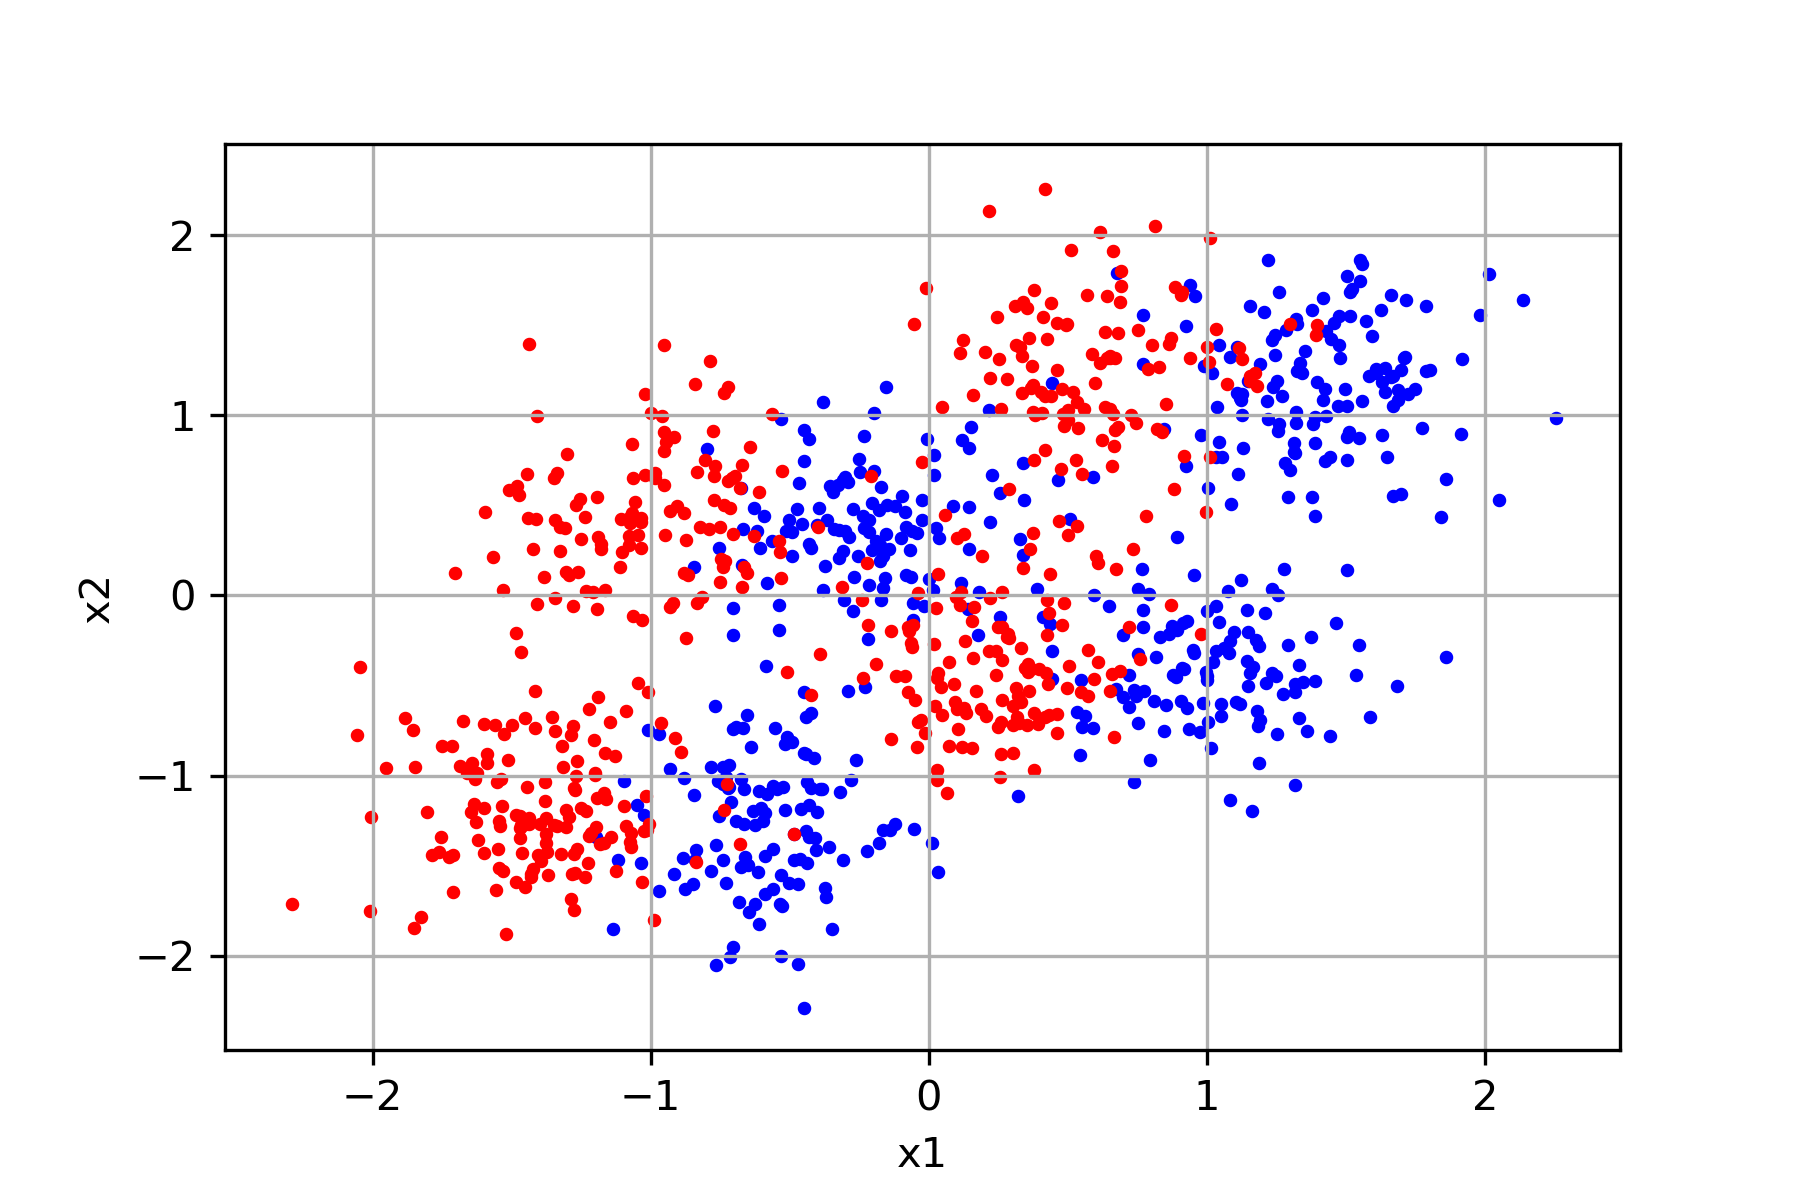
\includegraphics[width=12cm]{raw_data}
    \caption{}
    \label{fig:mlp-raw_data}
\end{figure}

\begin{figure}[H]
    \centering
    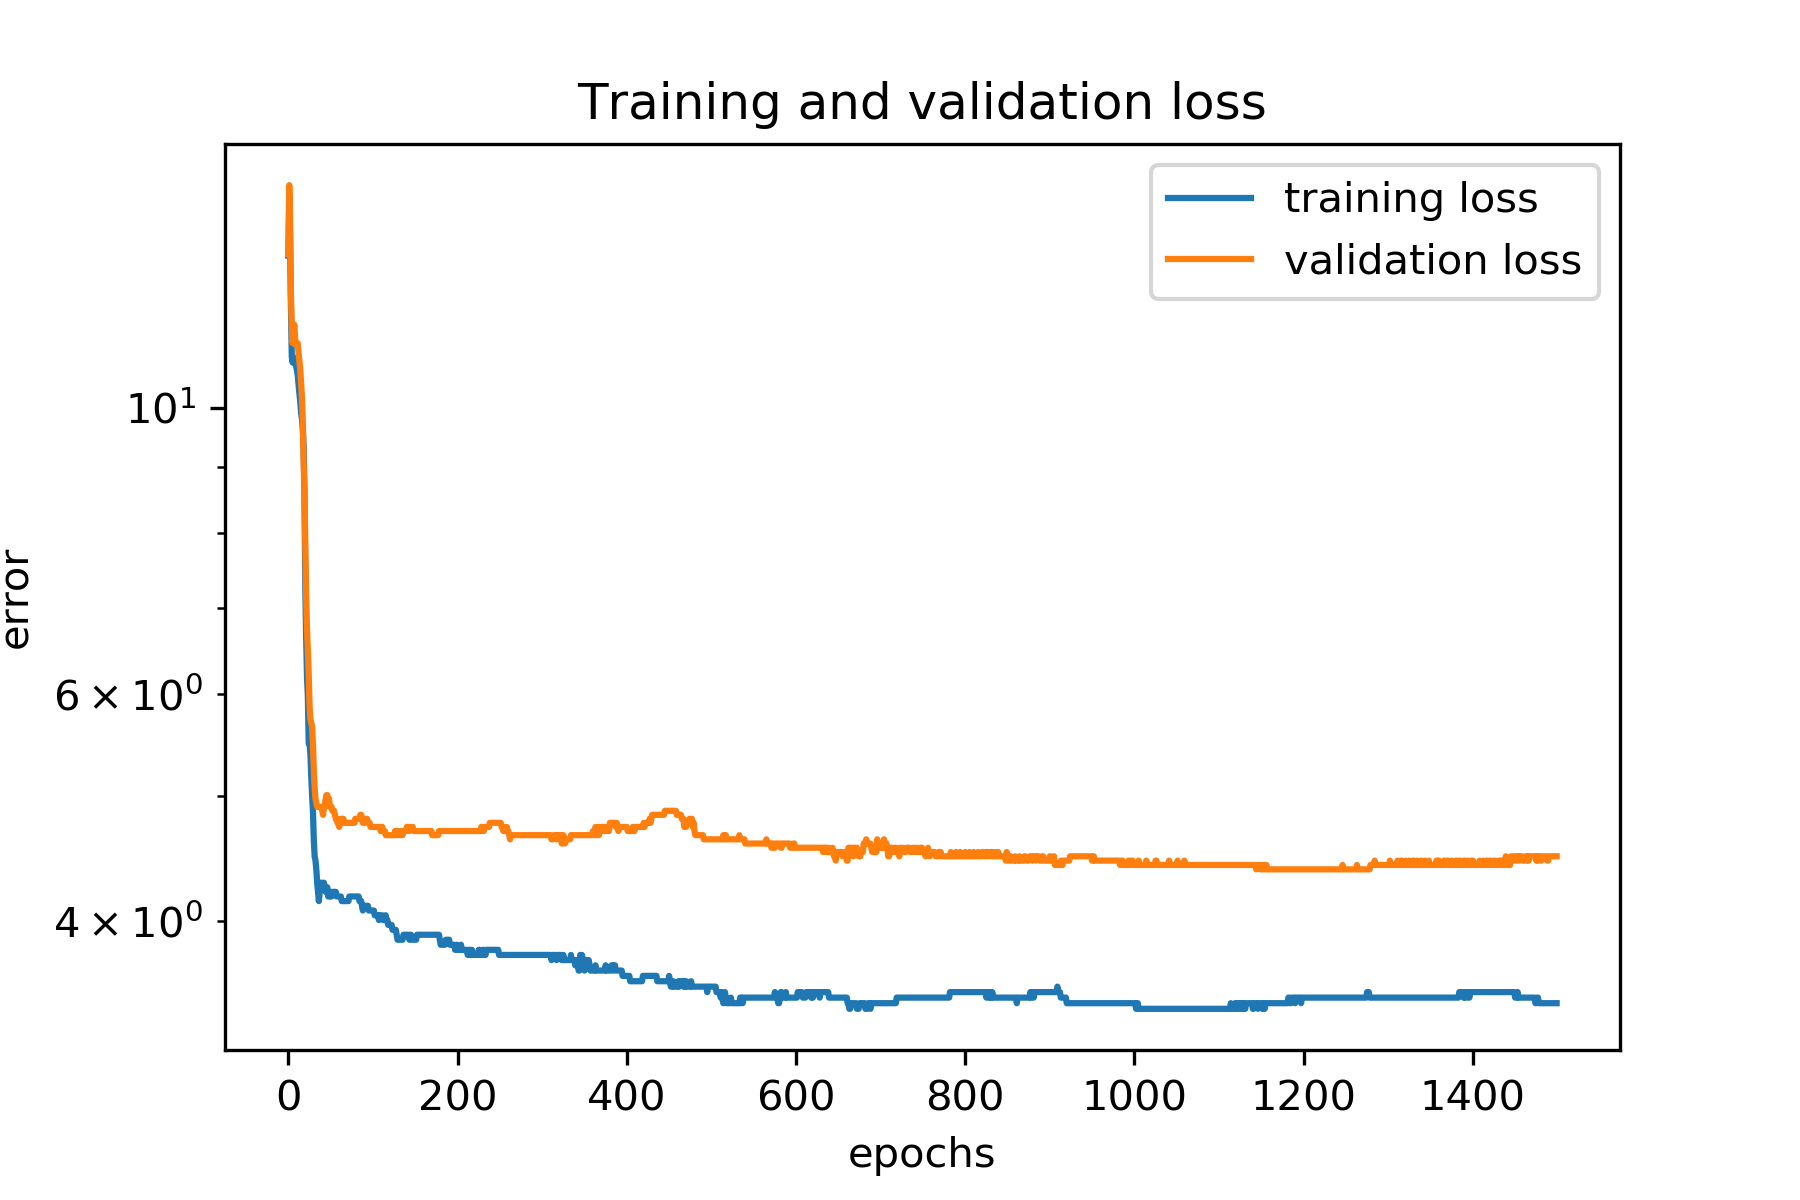
\includegraphics[width=12cm]{training_validation_loss}
    \caption{}
    \label{fig:mlp-training_validation_loss}
\end{figure}

\begin{figure}[H]
    \centering
    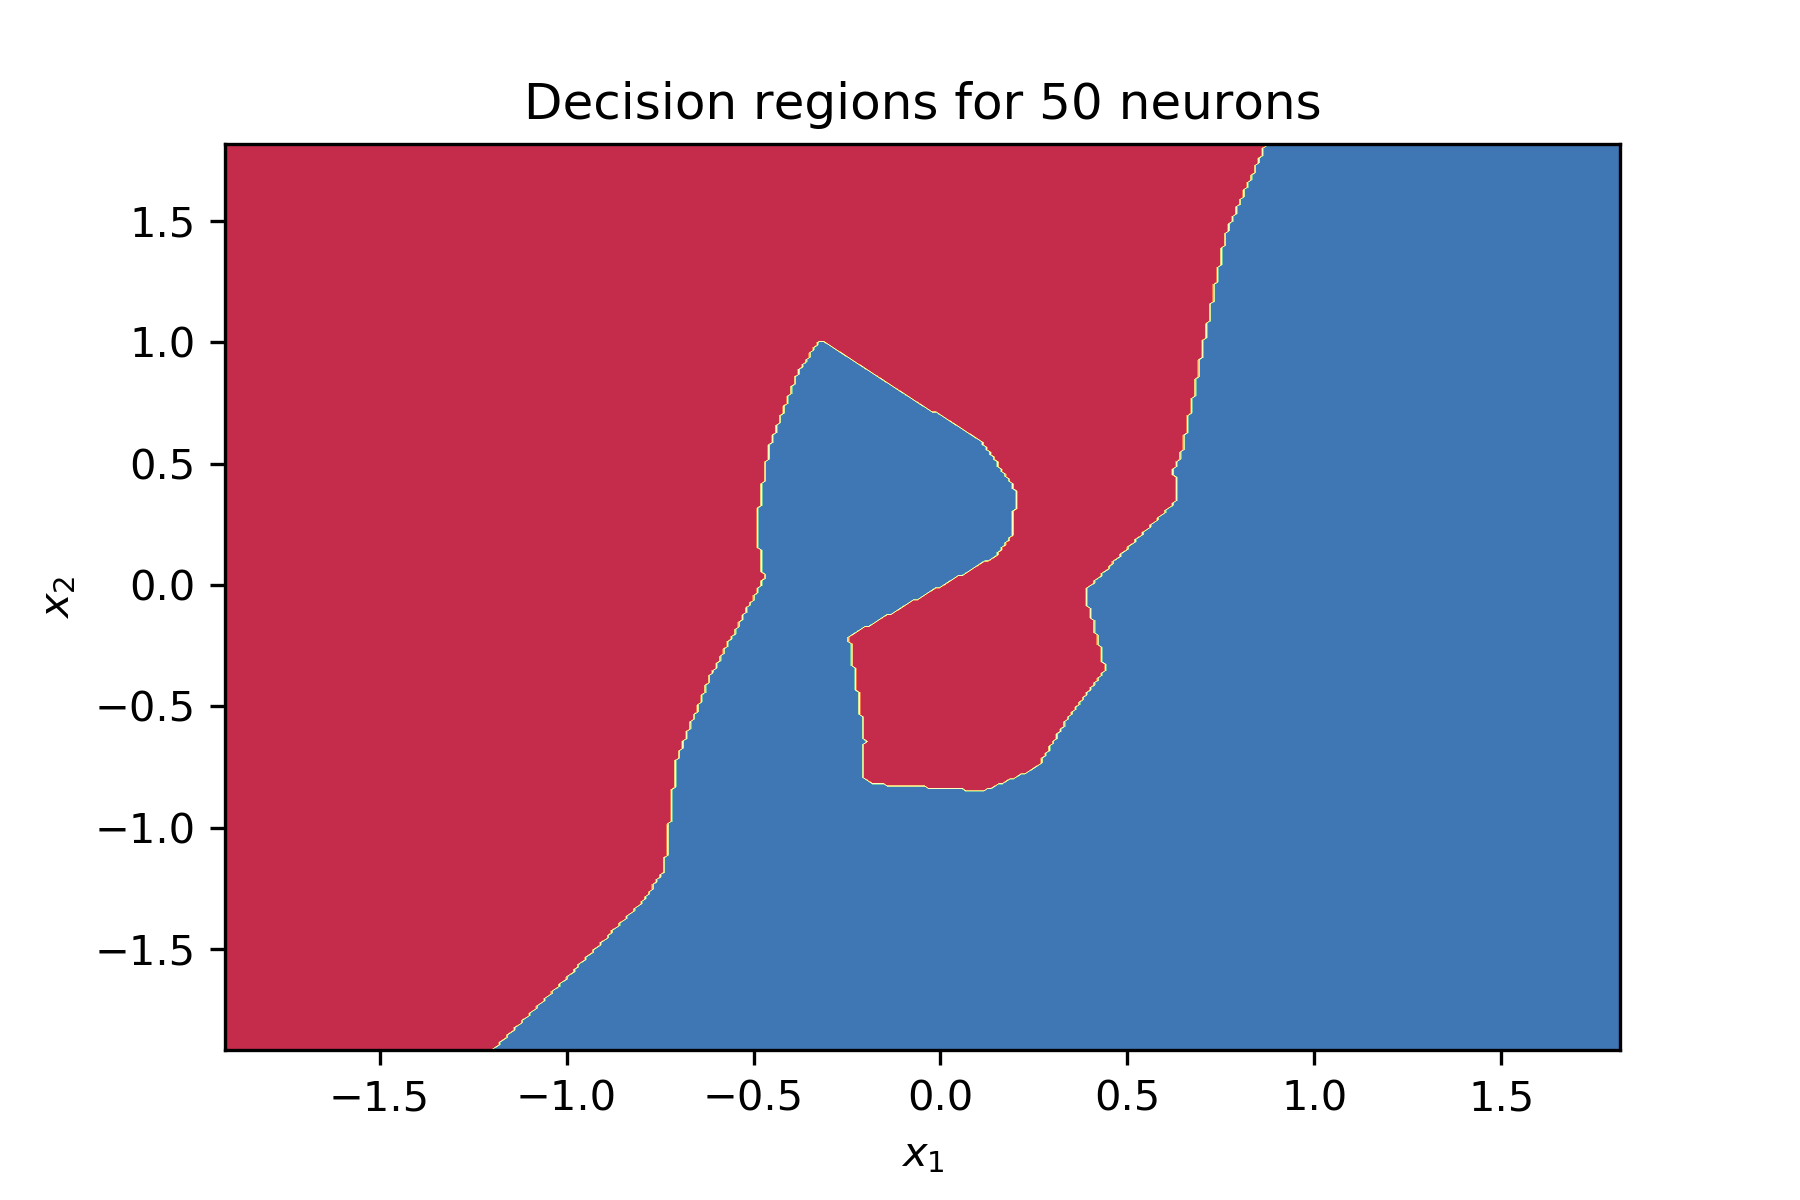
\includegraphics[width=12cm]{mlp_decision_region}
    \caption{}
    \label{fig:mlp-decision_regions}
\end{figure}

\begin{figure}[H]
    \centering
    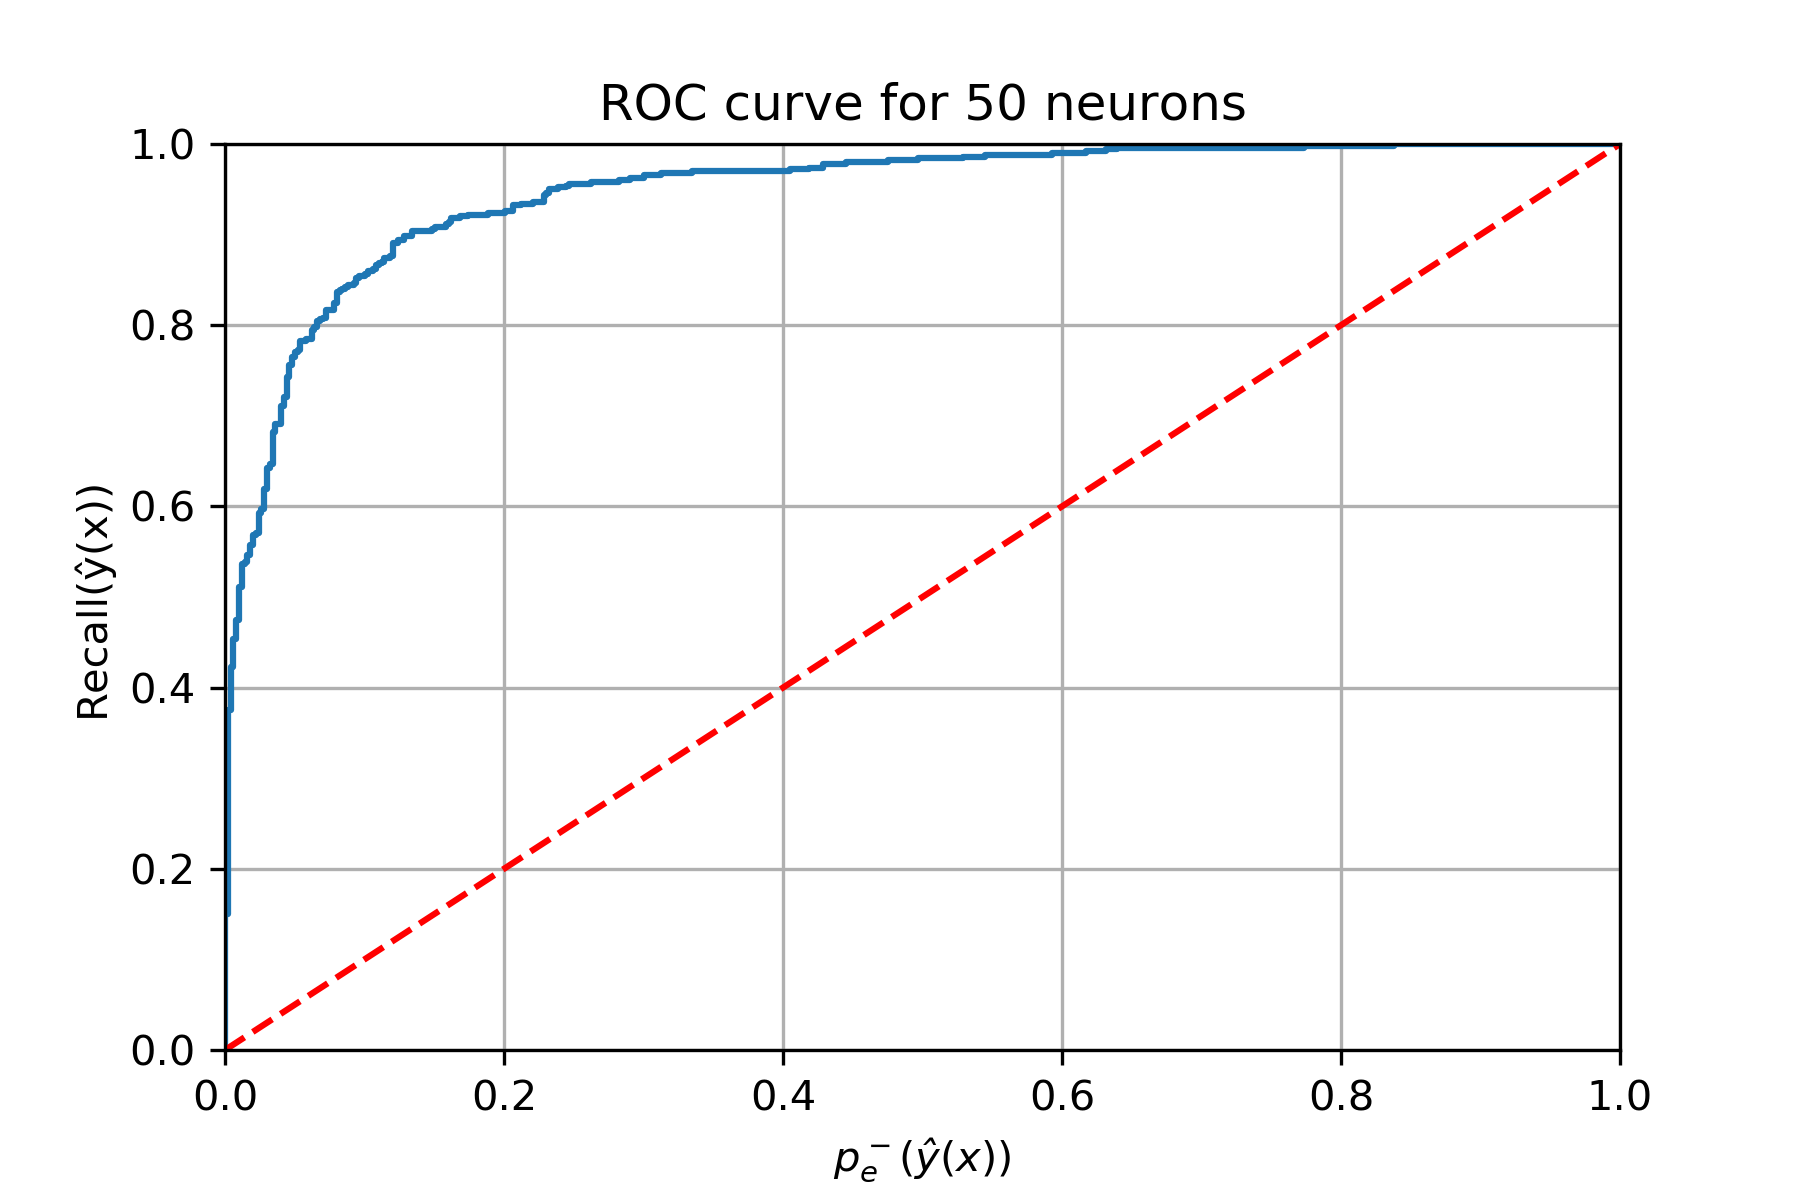
\includegraphics[width=12cm]{ROC_curve}
    \caption{}
    \label{fig:mlp-roc_curve}
\end{figure}

%-------------------------------------------------
%\newpage
% decision regions for different number of neurons

\begin{figure}[H]
    \centering
    % 5 neurons
    \begin{subfigure}{0.32\textwidth}
        \centering
        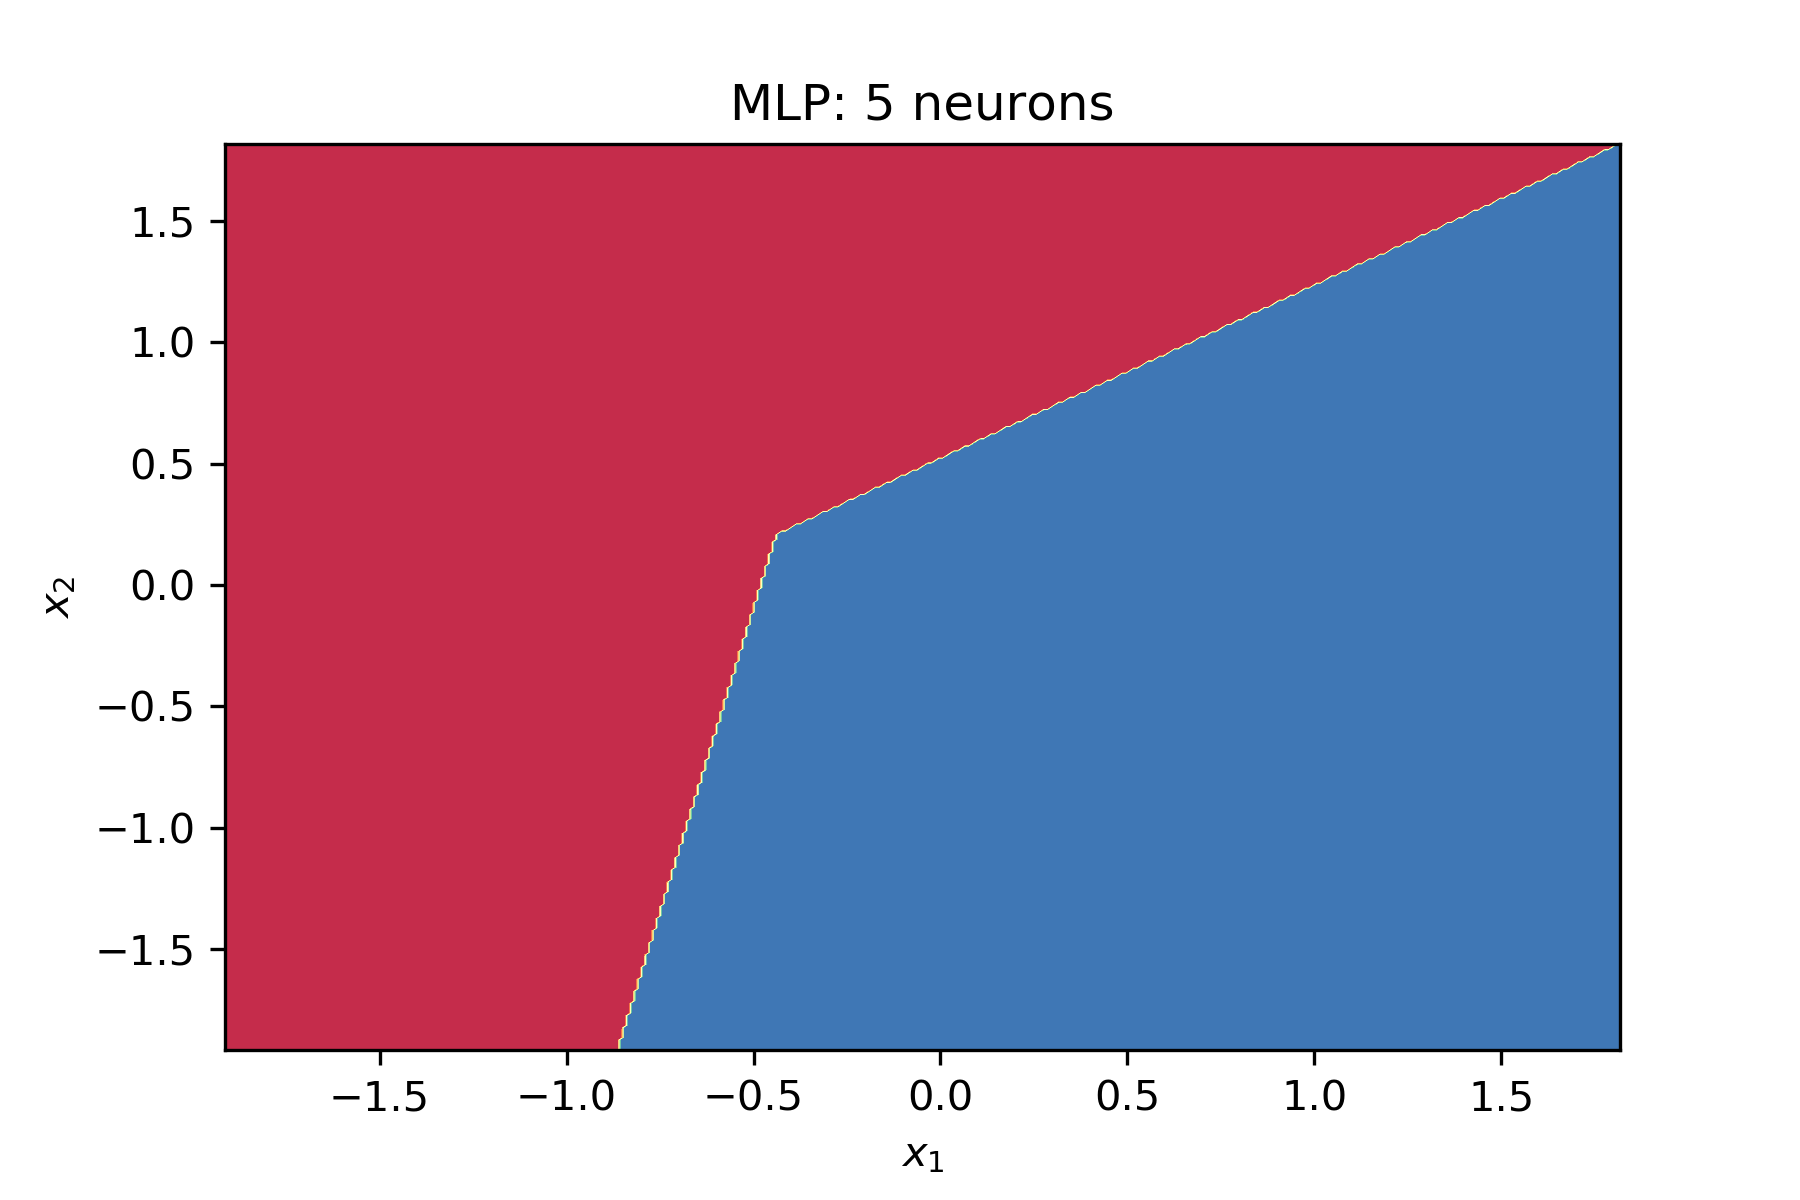
\includegraphics[width=3.85cm]{decision_regions_5}
        \caption{5 neurons}
        \label{fig:mlp-5_neurons}
    \end{subfigure}
    \hfill
    % 25 neurons
    \begin{subfigure}{0.32\textwidth}
        \centering
        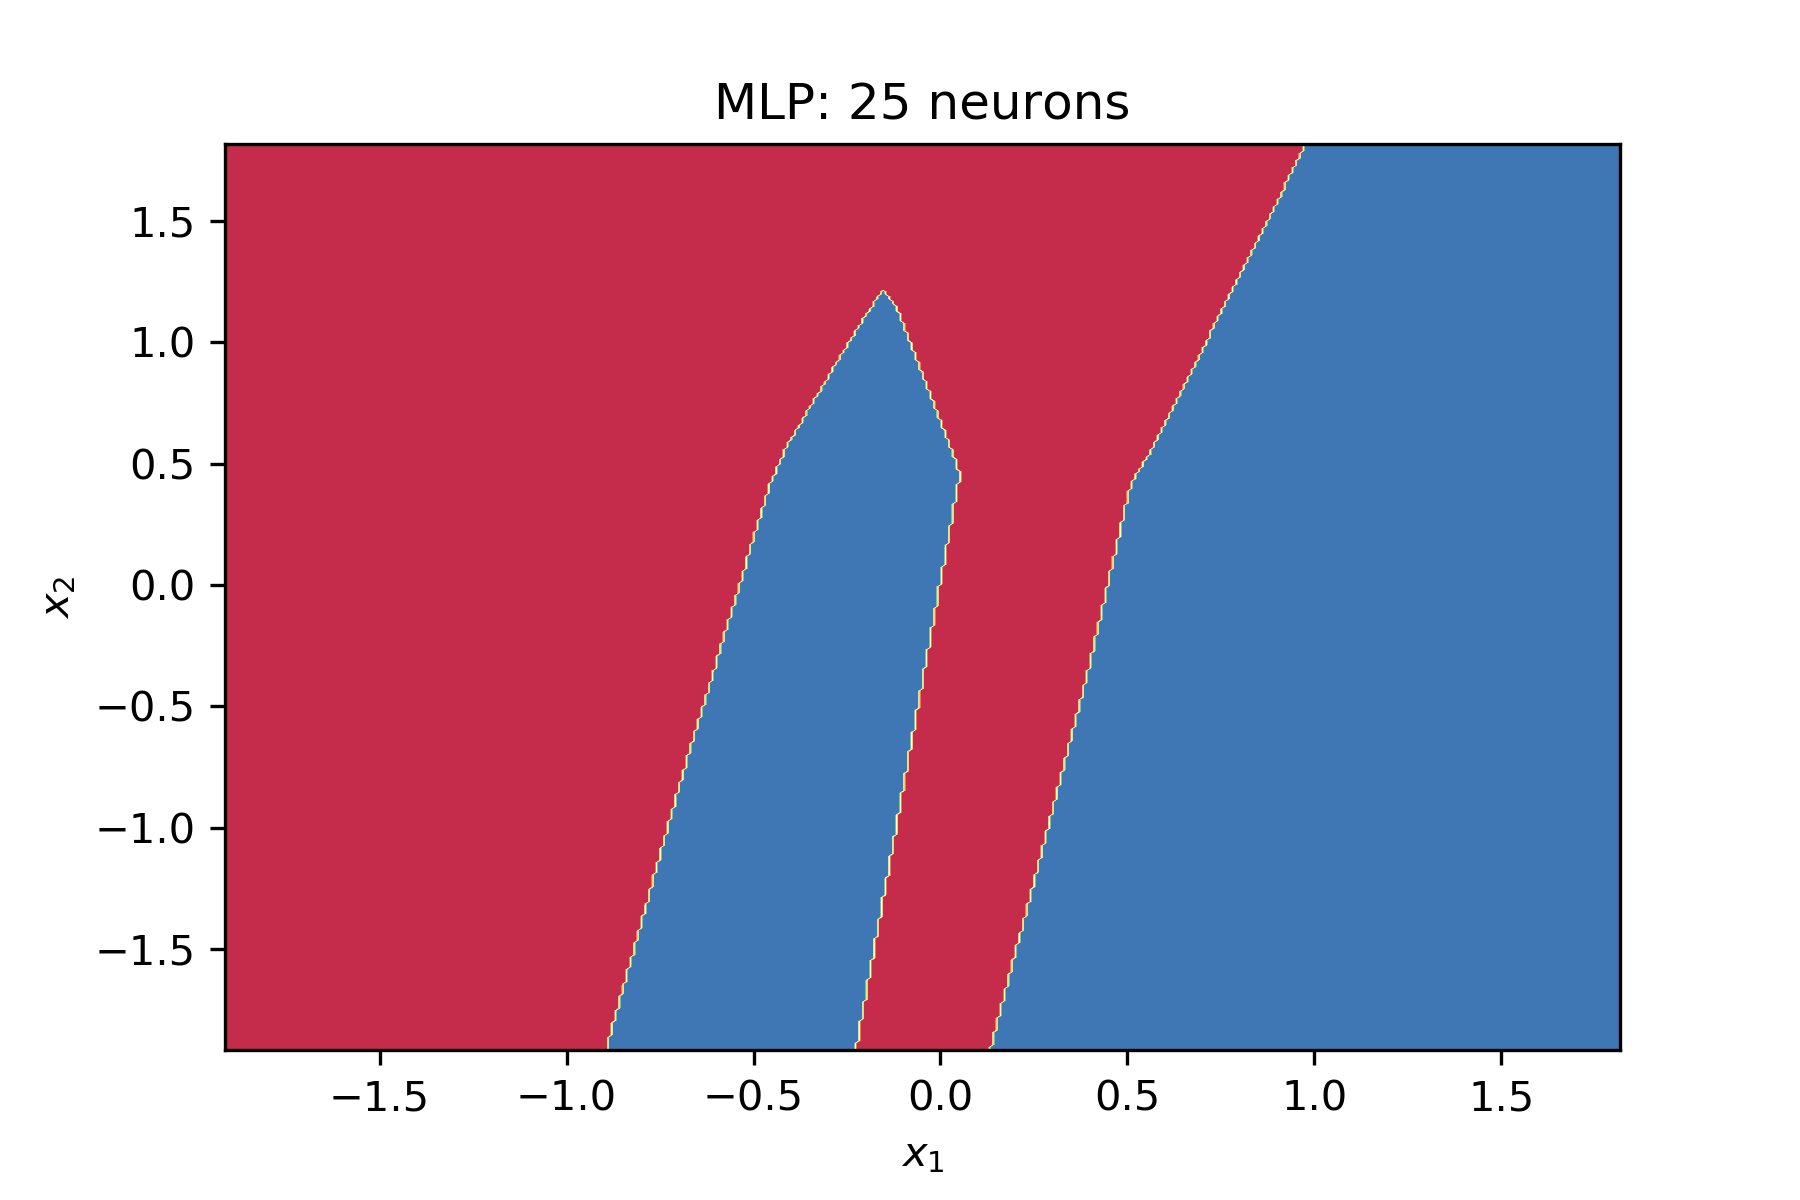
\includegraphics[width=3.85cm]{decision_regions_25}
        \caption{25 neurons}
        \label{fig:mlp-25_neurons}
    \end{subfigure}
    \hfill
    % 75 neurons
    \begin{subfigure}{0.32\textwidth}
        \centering
        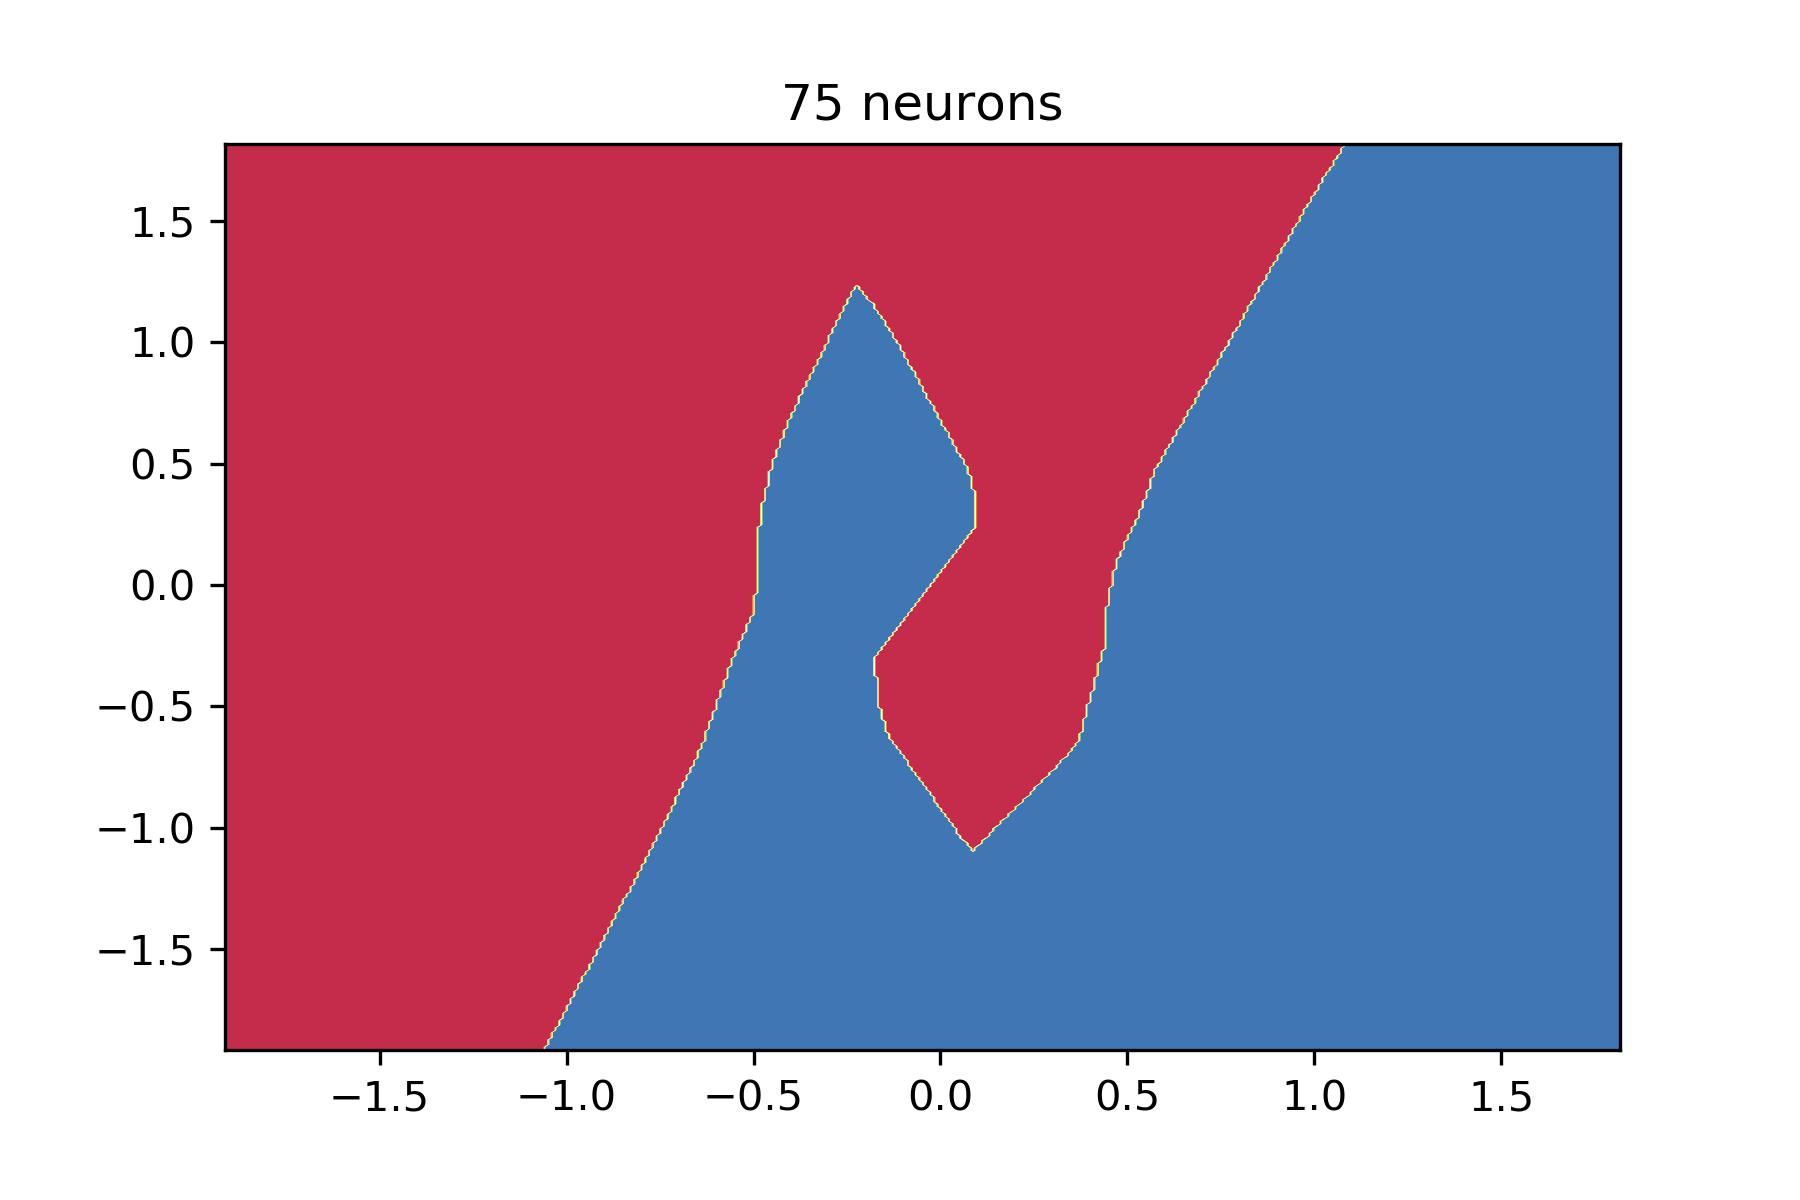
\includegraphics[width=3.85cm]{decision_regions_75}
        \caption{75 neurons}
        \label{fig:mlp-75_neurons}
    \end{subfigure}
    \hfill
    % 100 neurons
    \begin{subfigure}{0.32\textwidth}
        \centering
        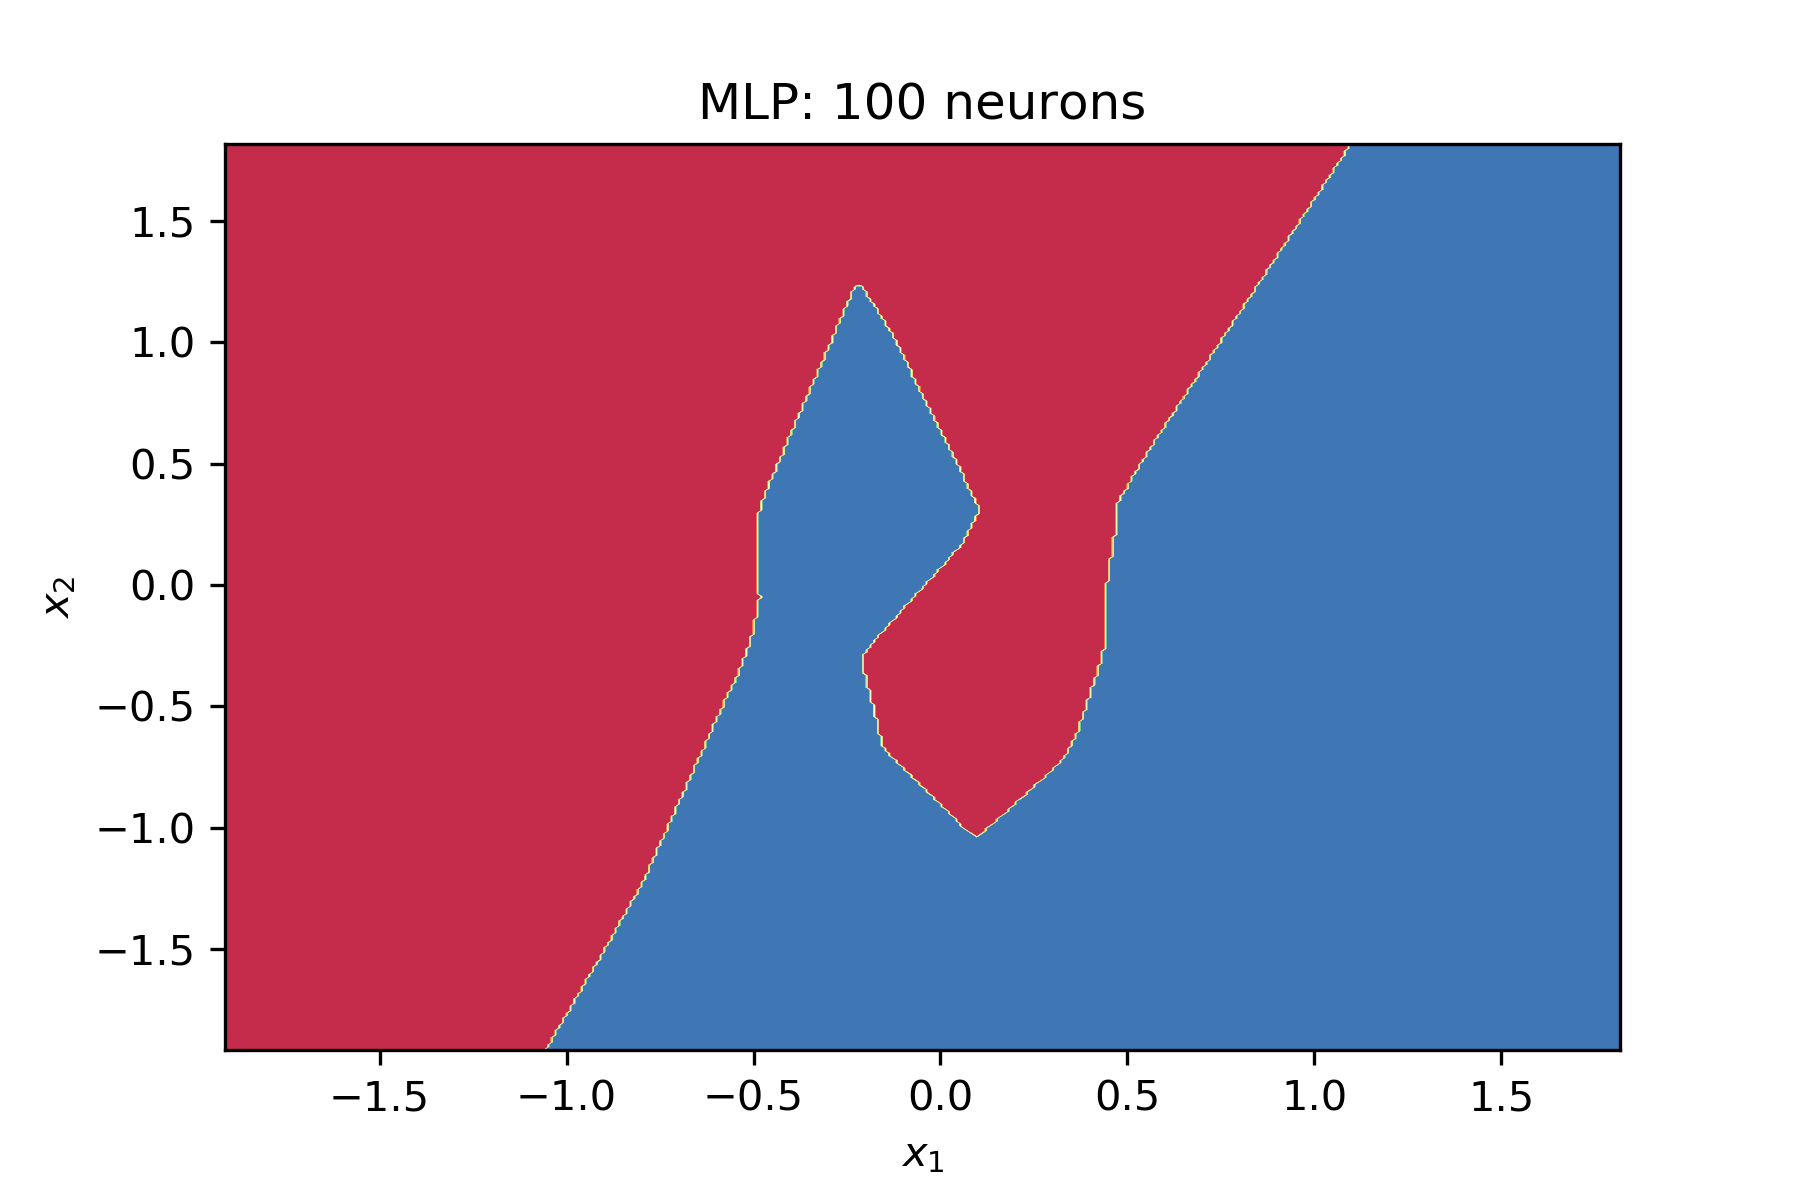
\includegraphics[width=3.85cm]{decision_regions_100}
        \caption{100 neurons}
        \label{fig:mlp-100_neurons}
    \end{subfigure}
    \hfill
    % 300 neurons
    \begin{subfigure}{0.32\textwidth}
        \centering
        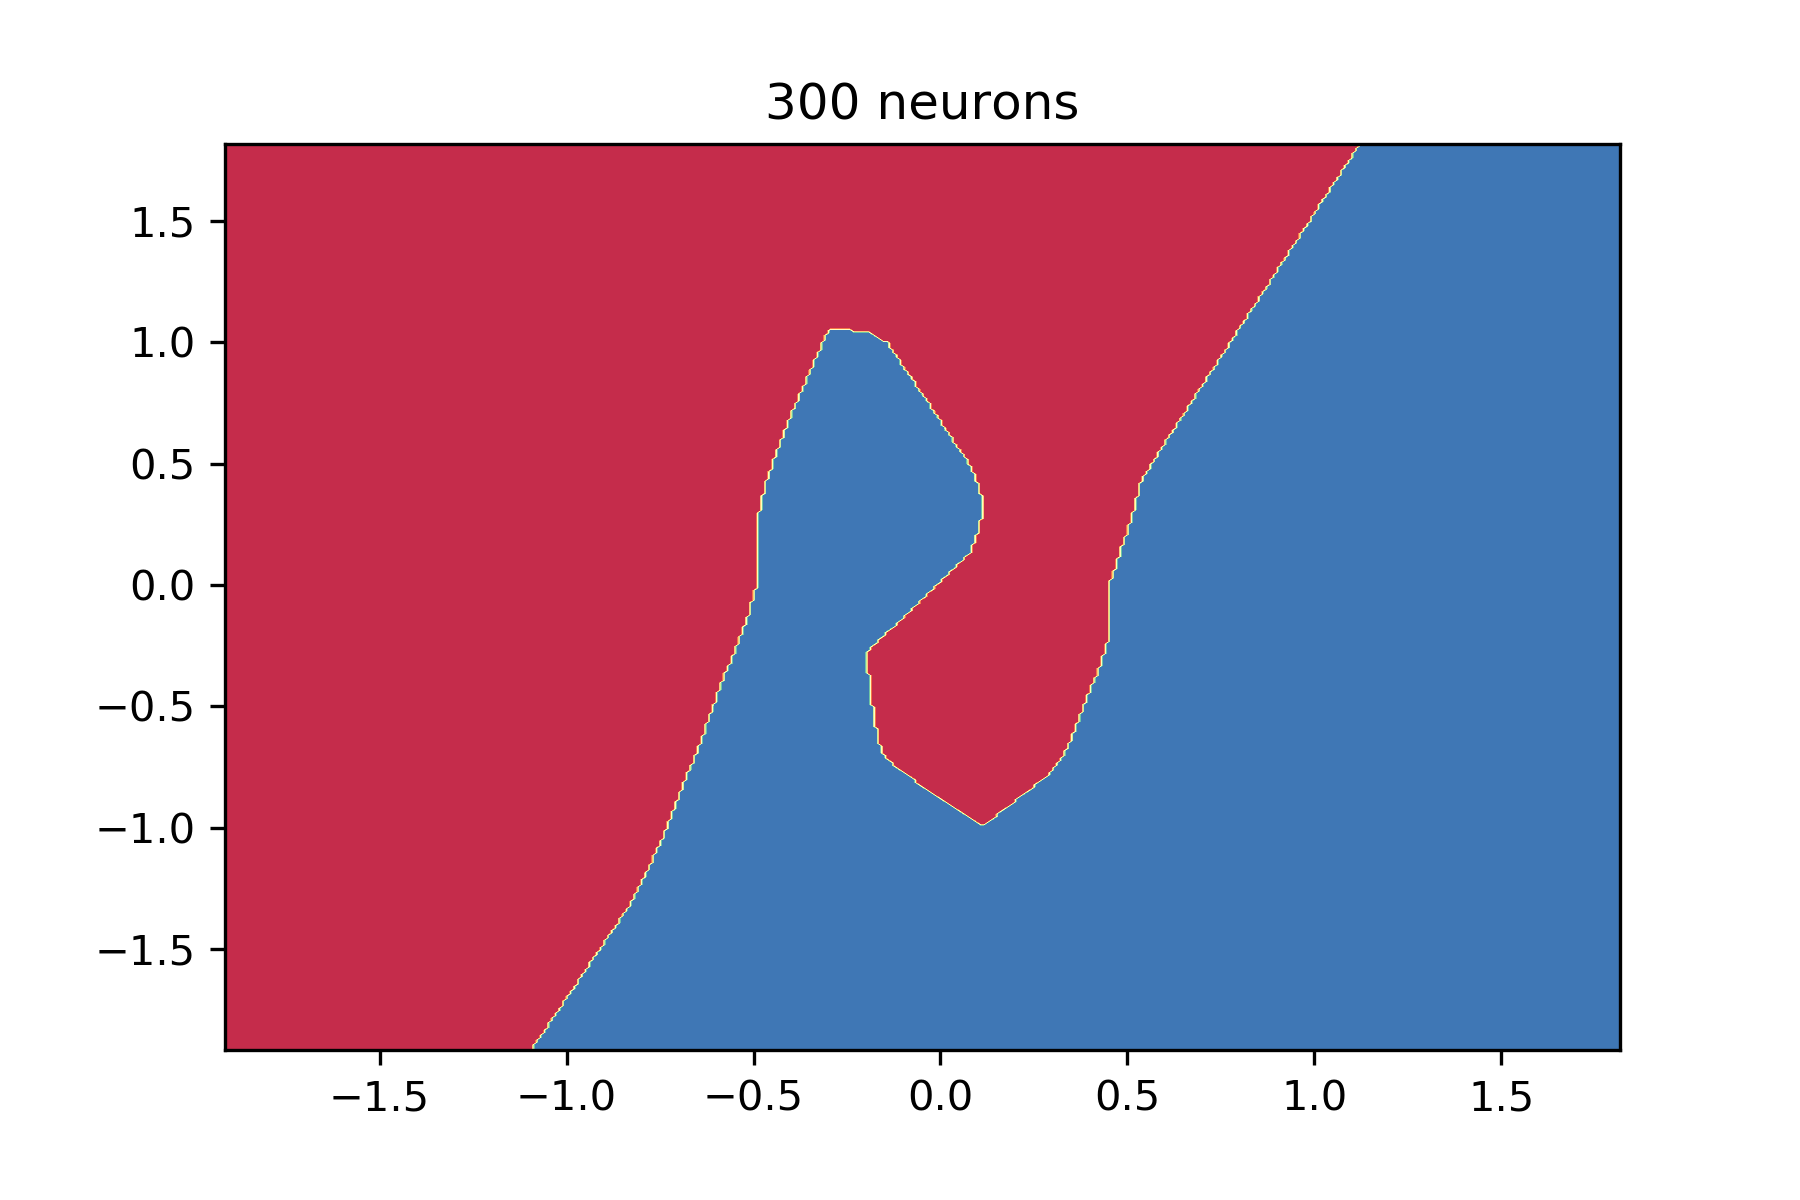
\includegraphics[width=3.85cm]{decision_regions_300}
        \caption{300 neurons}
        \label{fig:mlp-300_neurons}
    \end{subfigure}
    \hfill
    % 1000 neurons
    \begin{subfigure}{0.32\textwidth}
        \centering
        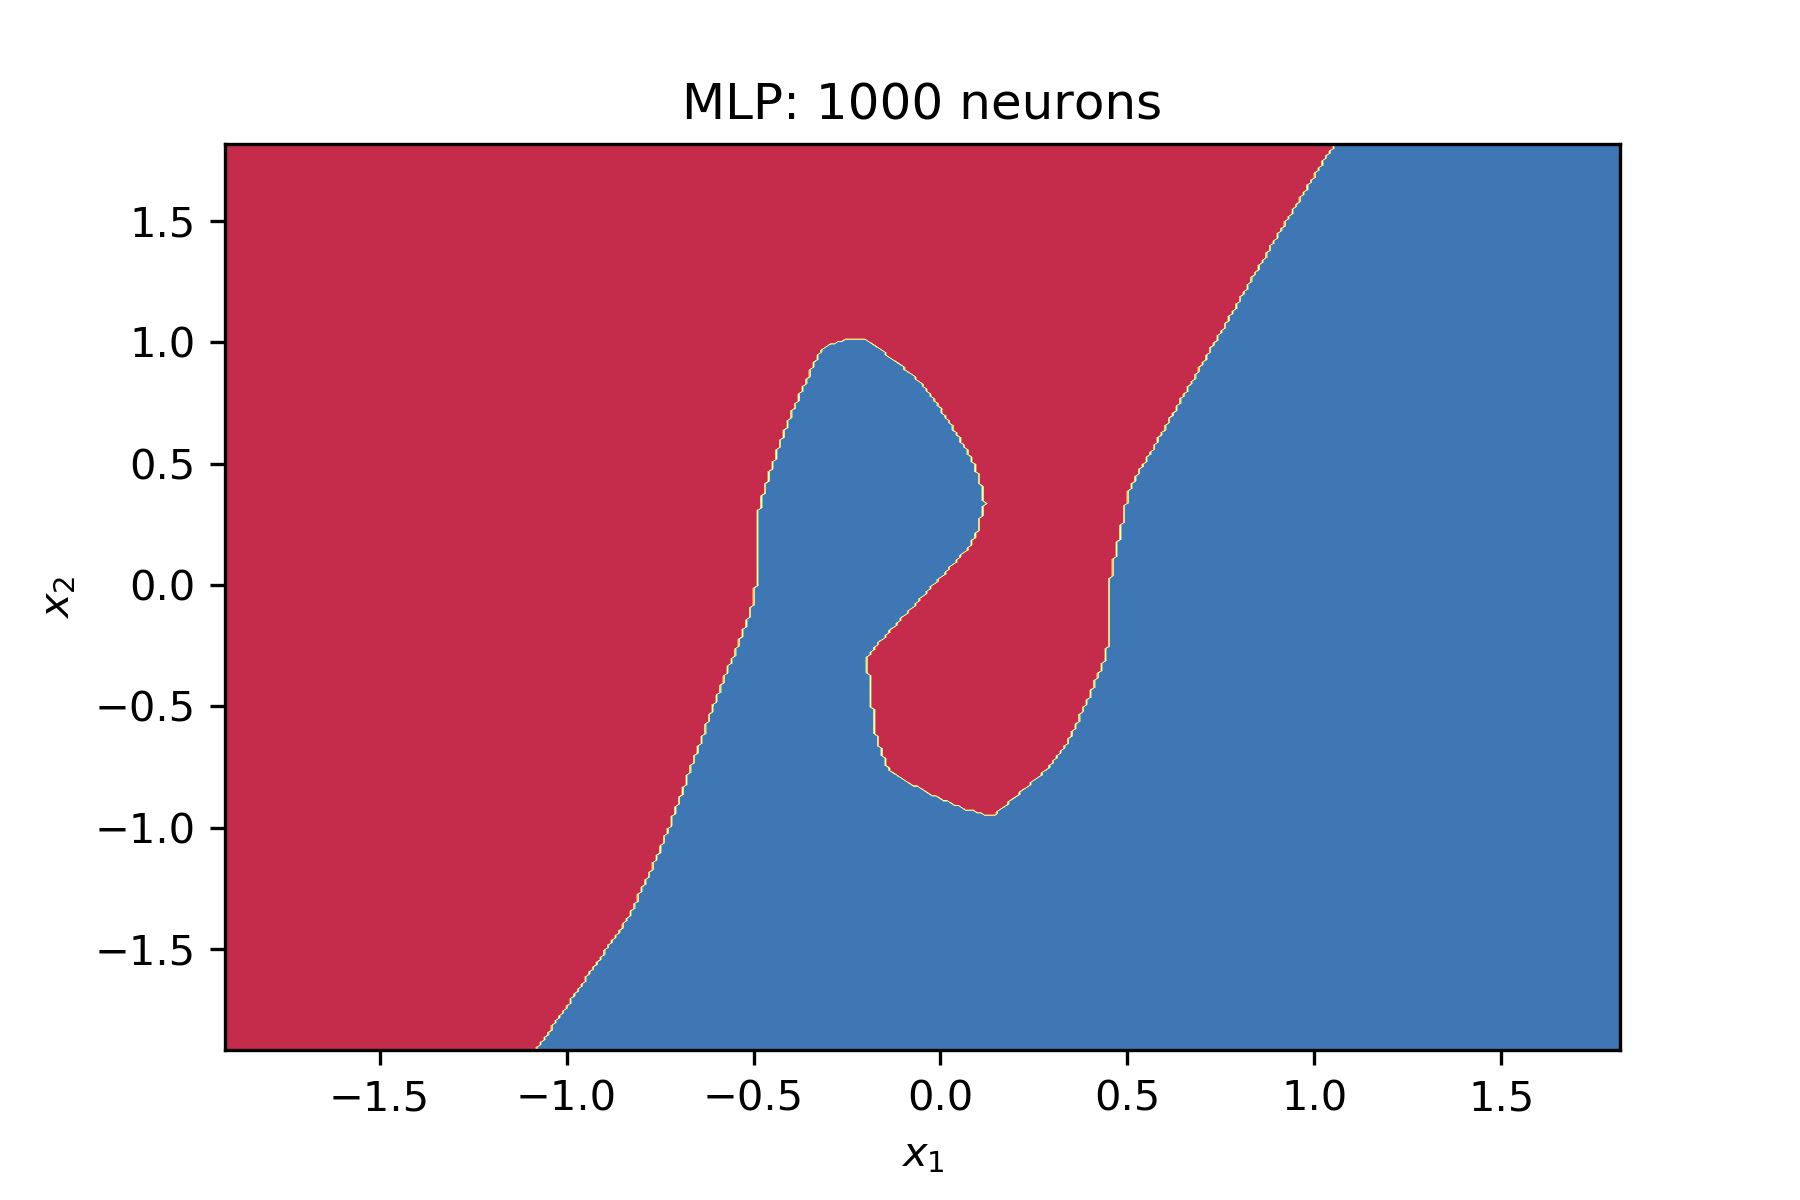
\includegraphics[width=3.85cm]{decision_regions_1000}
        \caption{1000 neurons}
        \label{fig:mlp-1000_neurons}
    \end{subfigure}
    \hfill
    % 5000 neurons
    \begin{subfigure}{0.32\textwidth}
        \centering
        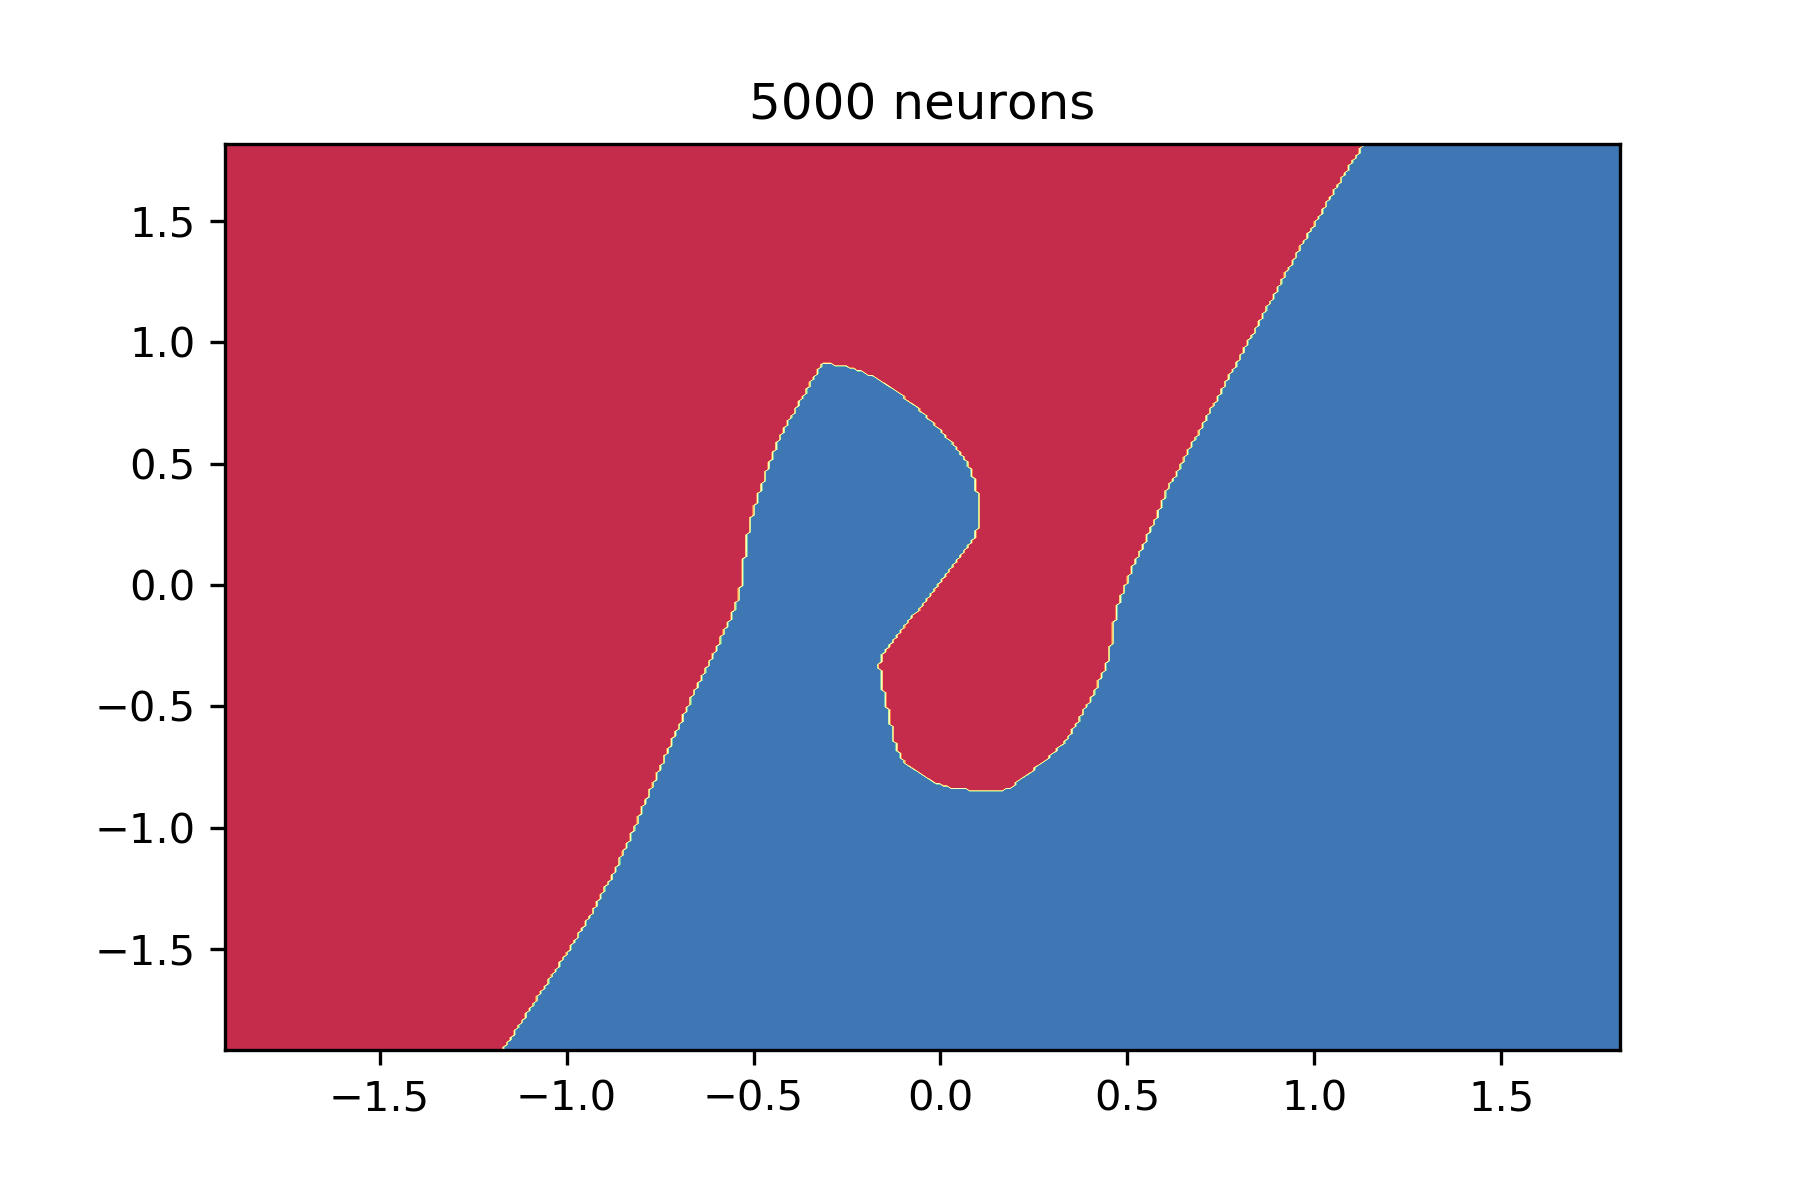
\includegraphics[width=3.85cm]{decision_regions_5000}
        \caption{5000 neurons}
        \label{fig:mlp-5000_neurons}
    \end{subfigure}
    \hfill
    % caption and label
    \caption{Decision regions for MLP with different number of neurons}
    \label{fig:mlp-decision_regions_N_neurons}
\end{figure}
%-------------------------------------------------



%-------------------------------------------------
%\newpage
% ROC curve for different number of neurons

\begin{figure}[H]
    \centering
    % 5 neurons
    \begin{subfigure}{0.32\textwidth}
        \centering
        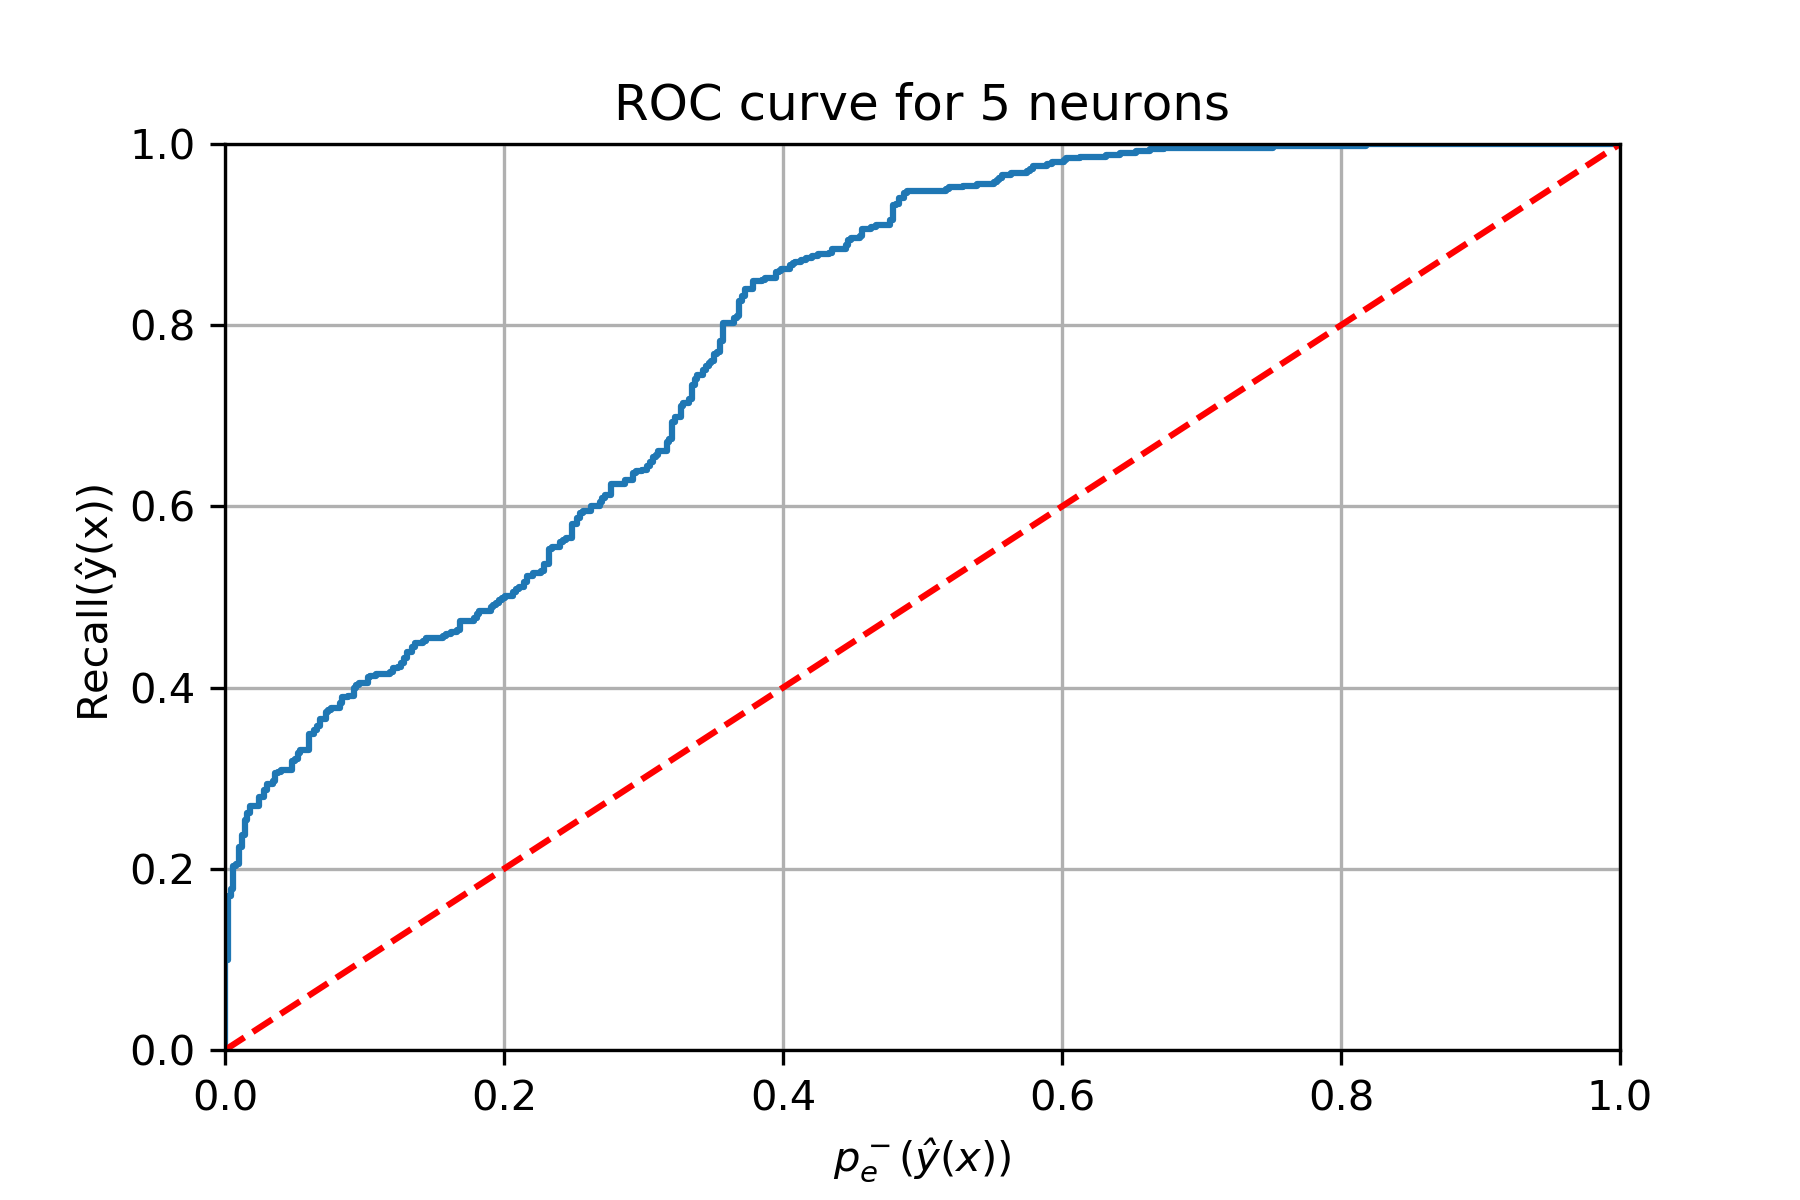
\includegraphics[width=3.85cm]{ROC_5}
        \caption{5 neurons}
        \label{fig:mlp-5_roc}
    \end{subfigure}
    \hfill
    % 25 neurons
    \begin{subfigure}{0.32\textwidth}
        \centering
        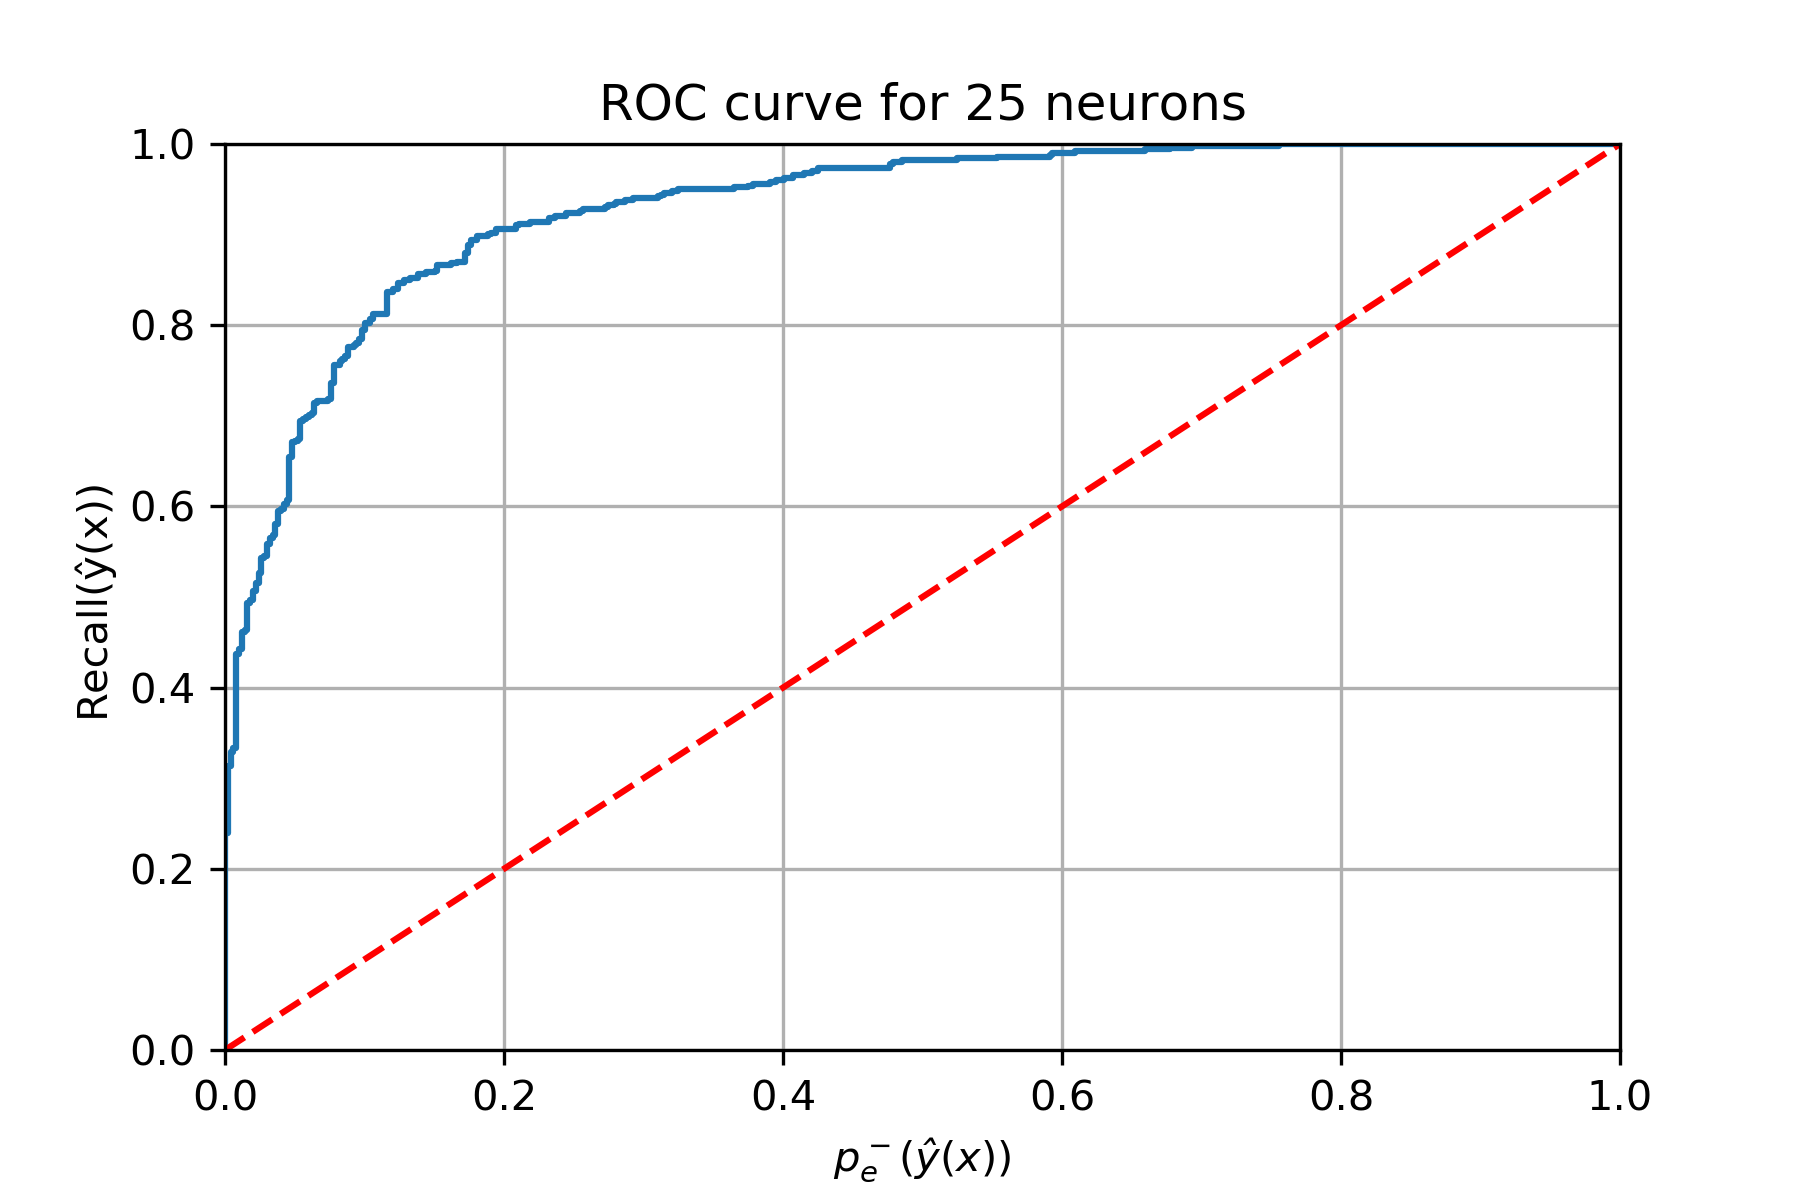
\includegraphics[width=3.85cm]{ROC_25}
        \caption{25 neurons}
        \label{fig:mlp-25_roc}
    \end{subfigure}
    \hfill
    % 75 neurons
    \begin{subfigure}{0.32\textwidth}
        \centering
        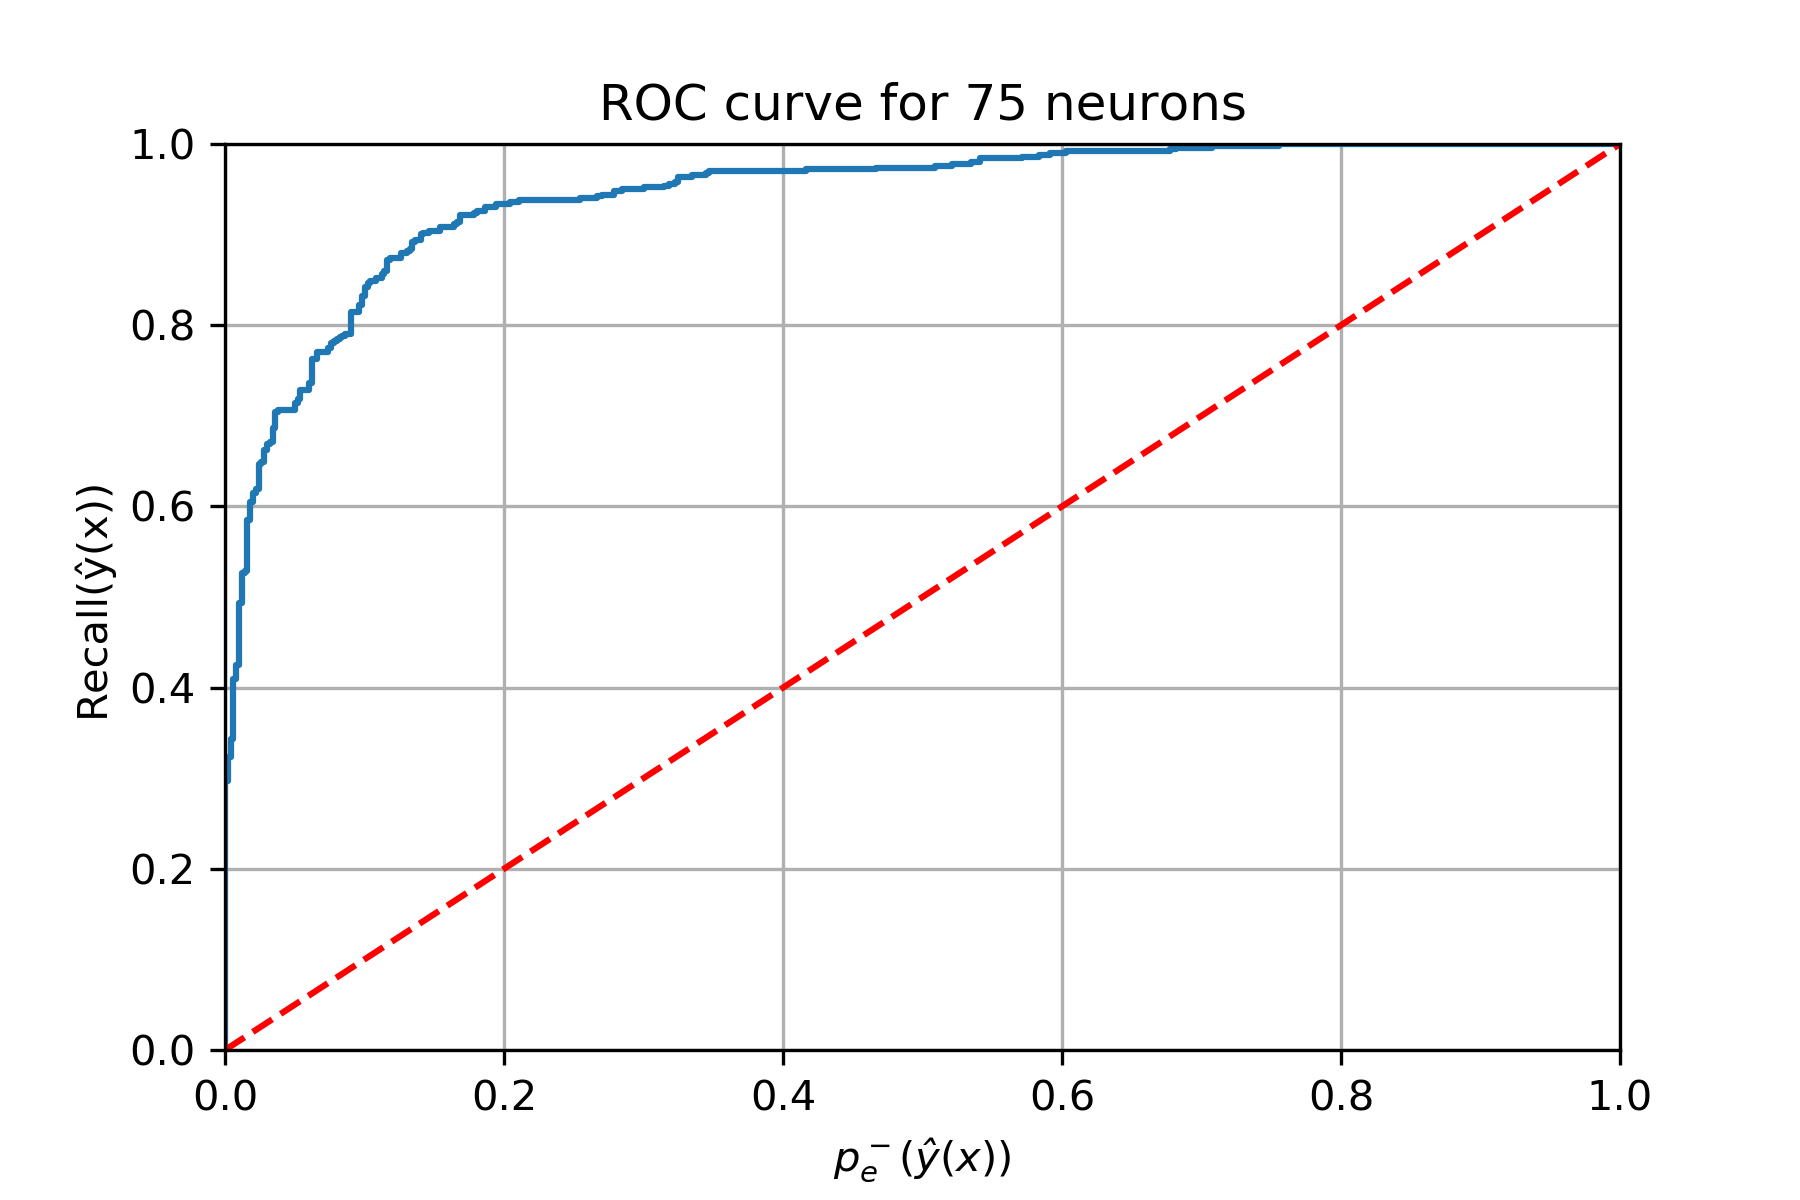
\includegraphics[width=3.85cm]{ROC_75}
        \caption{75 neurons}
        \label{fig:mlp-75_roc}
    \end{subfigure}
    \hfill
    % 100 neurons
    \begin{subfigure}{0.32\textwidth}
        \centering
        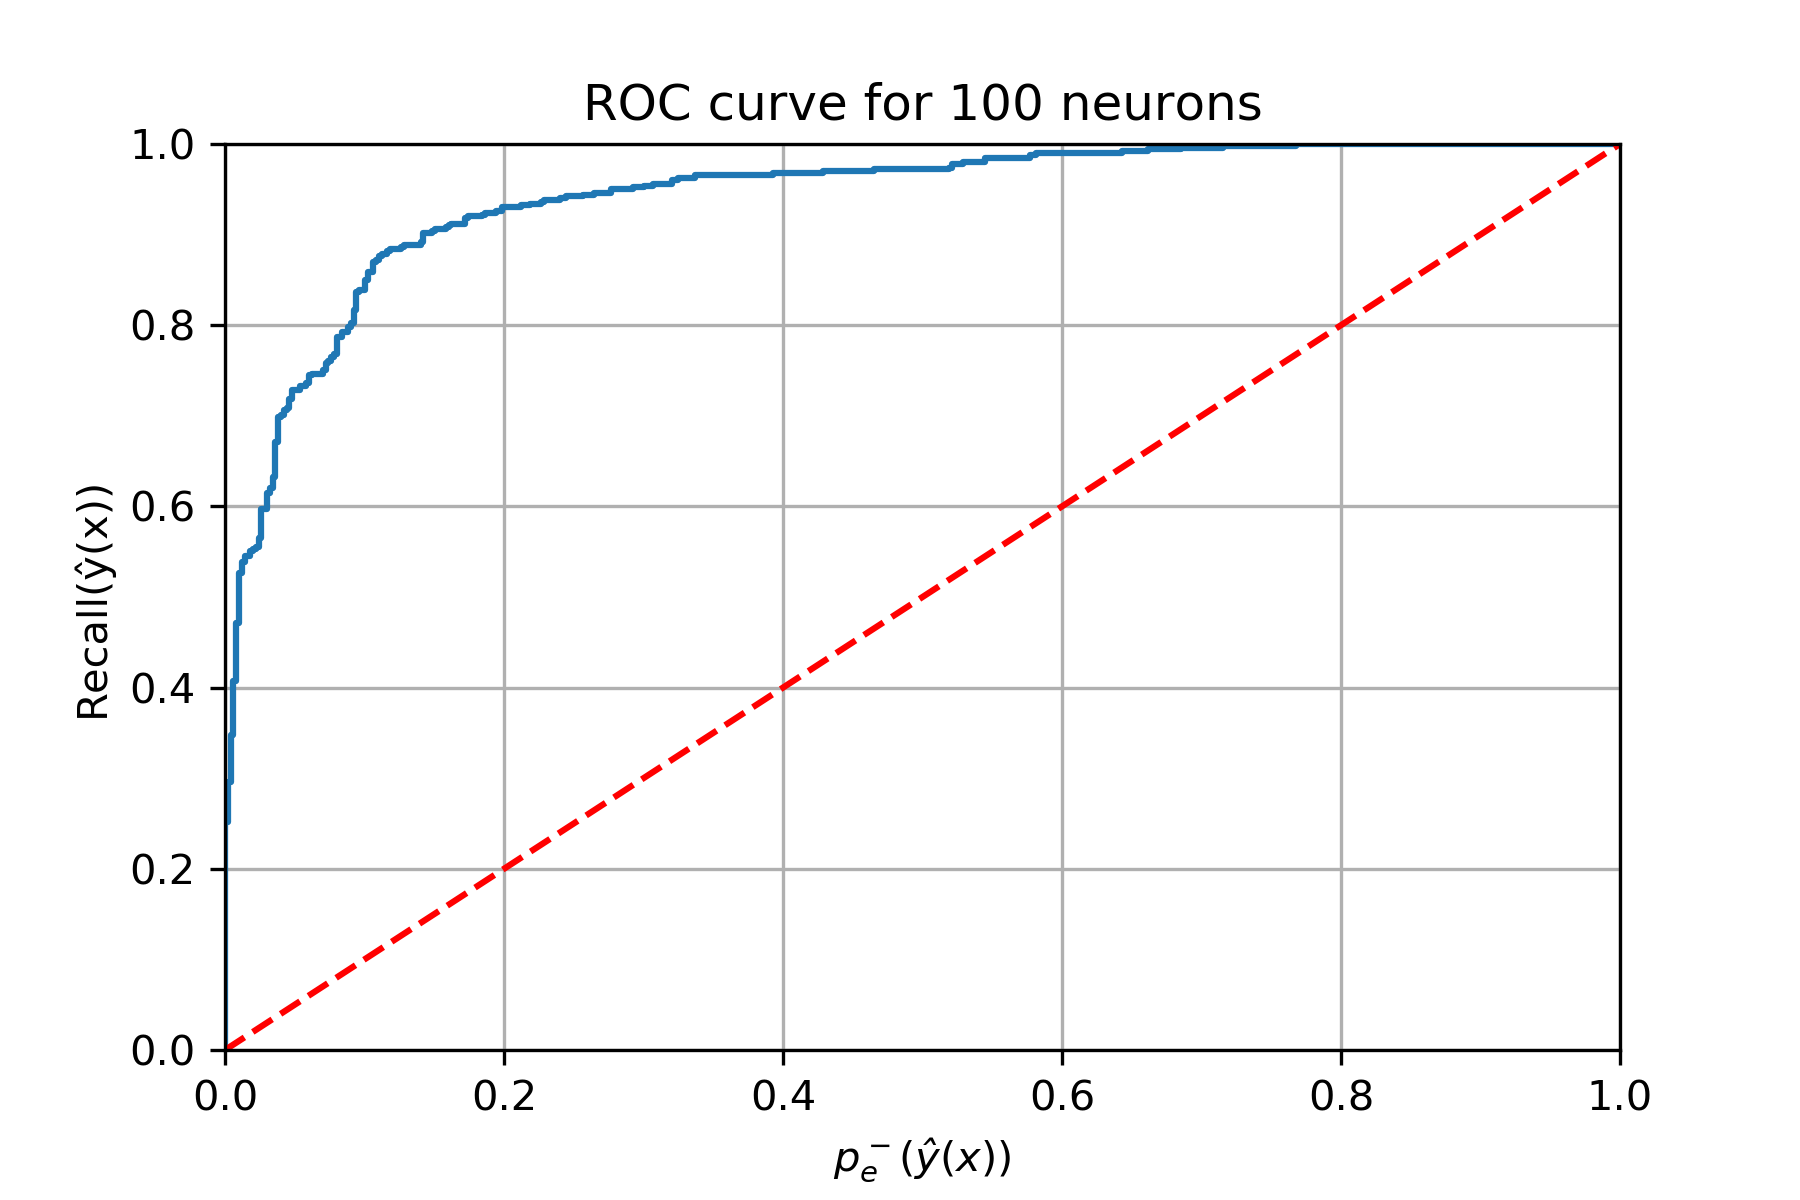
\includegraphics[width=3.85cm]{ROC_100}
        \caption{100 neurons}
        \label{fig:mlp-100_roc}
    \end{subfigure}
    \hfill
    % 300 neurons
    \begin{subfigure}{0.32\textwidth}
        \centering
        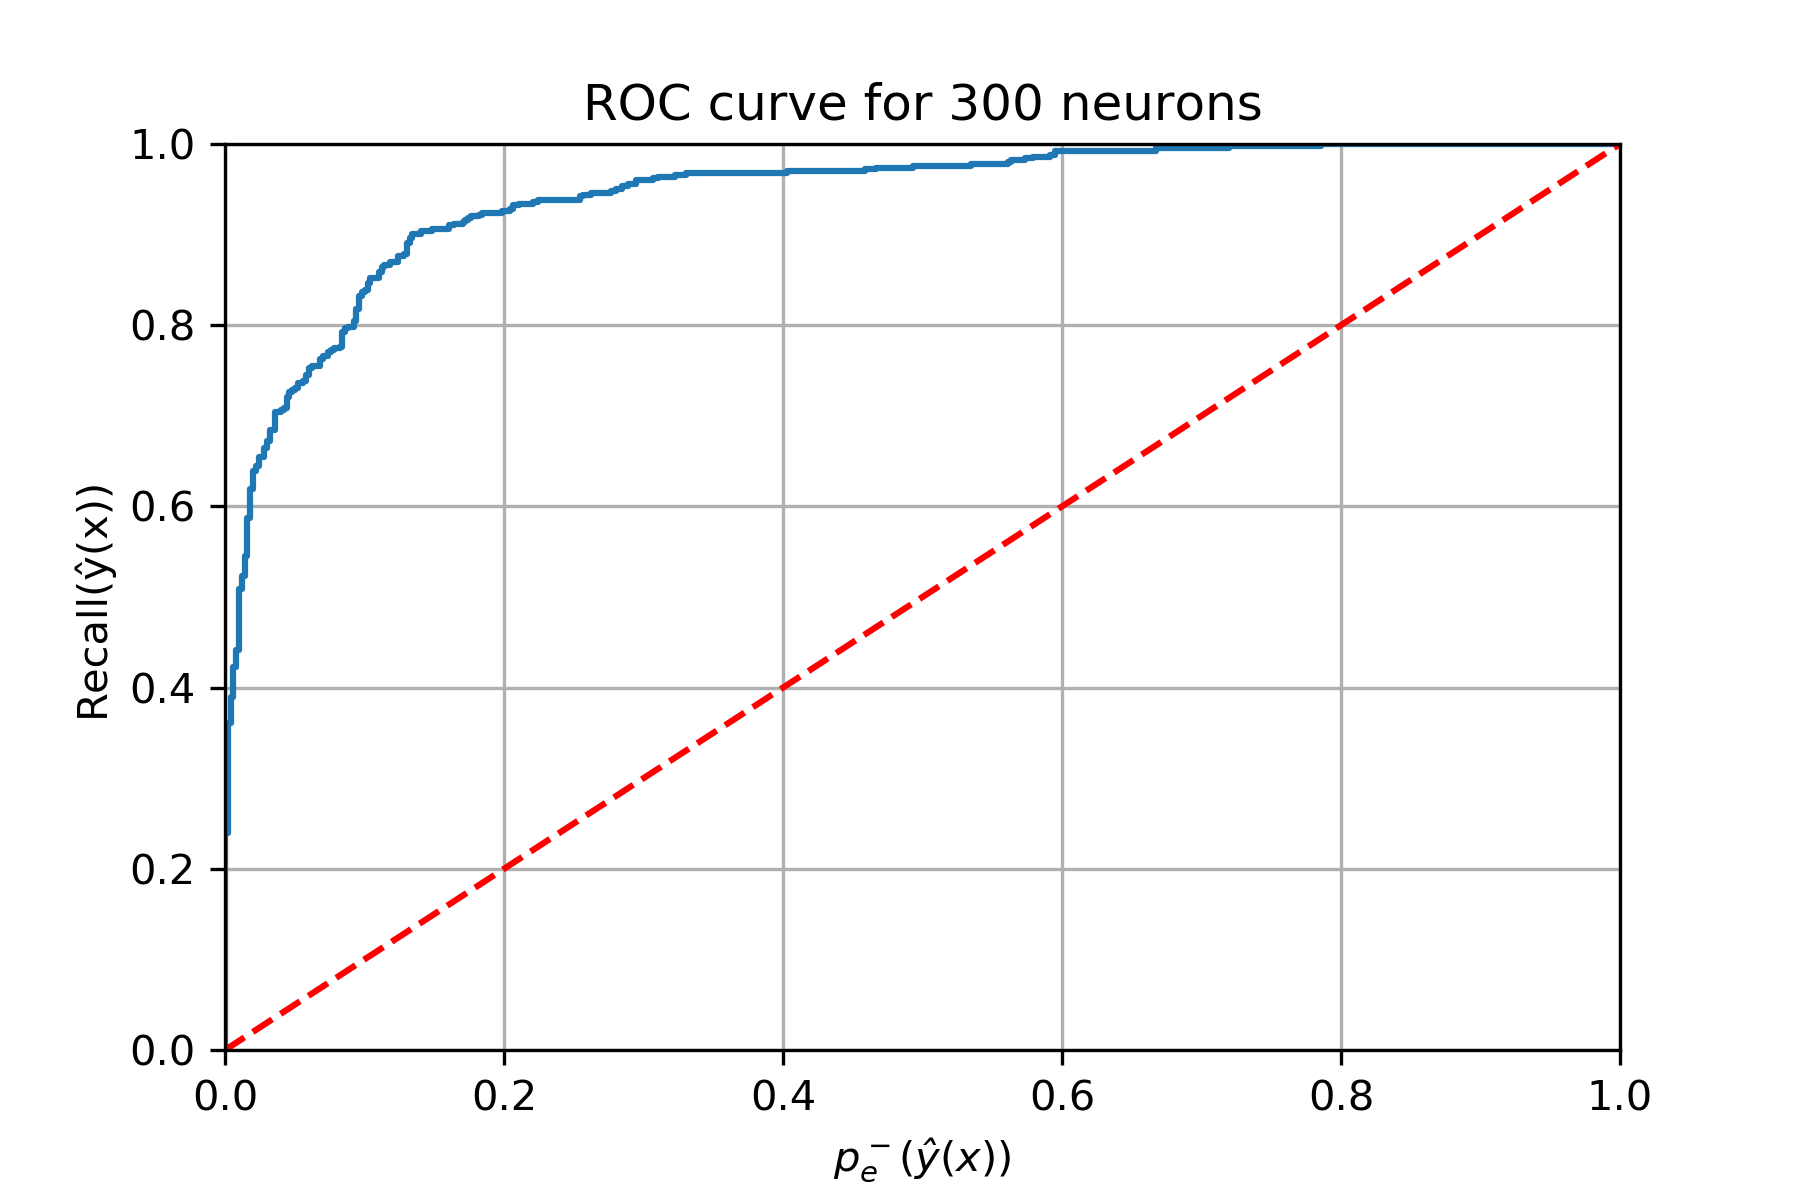
\includegraphics[width=3.85cm]{ROC_300}
        \caption{300 neurons}
        \label{fig:mlp-300_roc}
    \end{subfigure}
    \hfill
    % 1000 neurons
    \begin{subfigure}{0.32\textwidth}
        \centering
        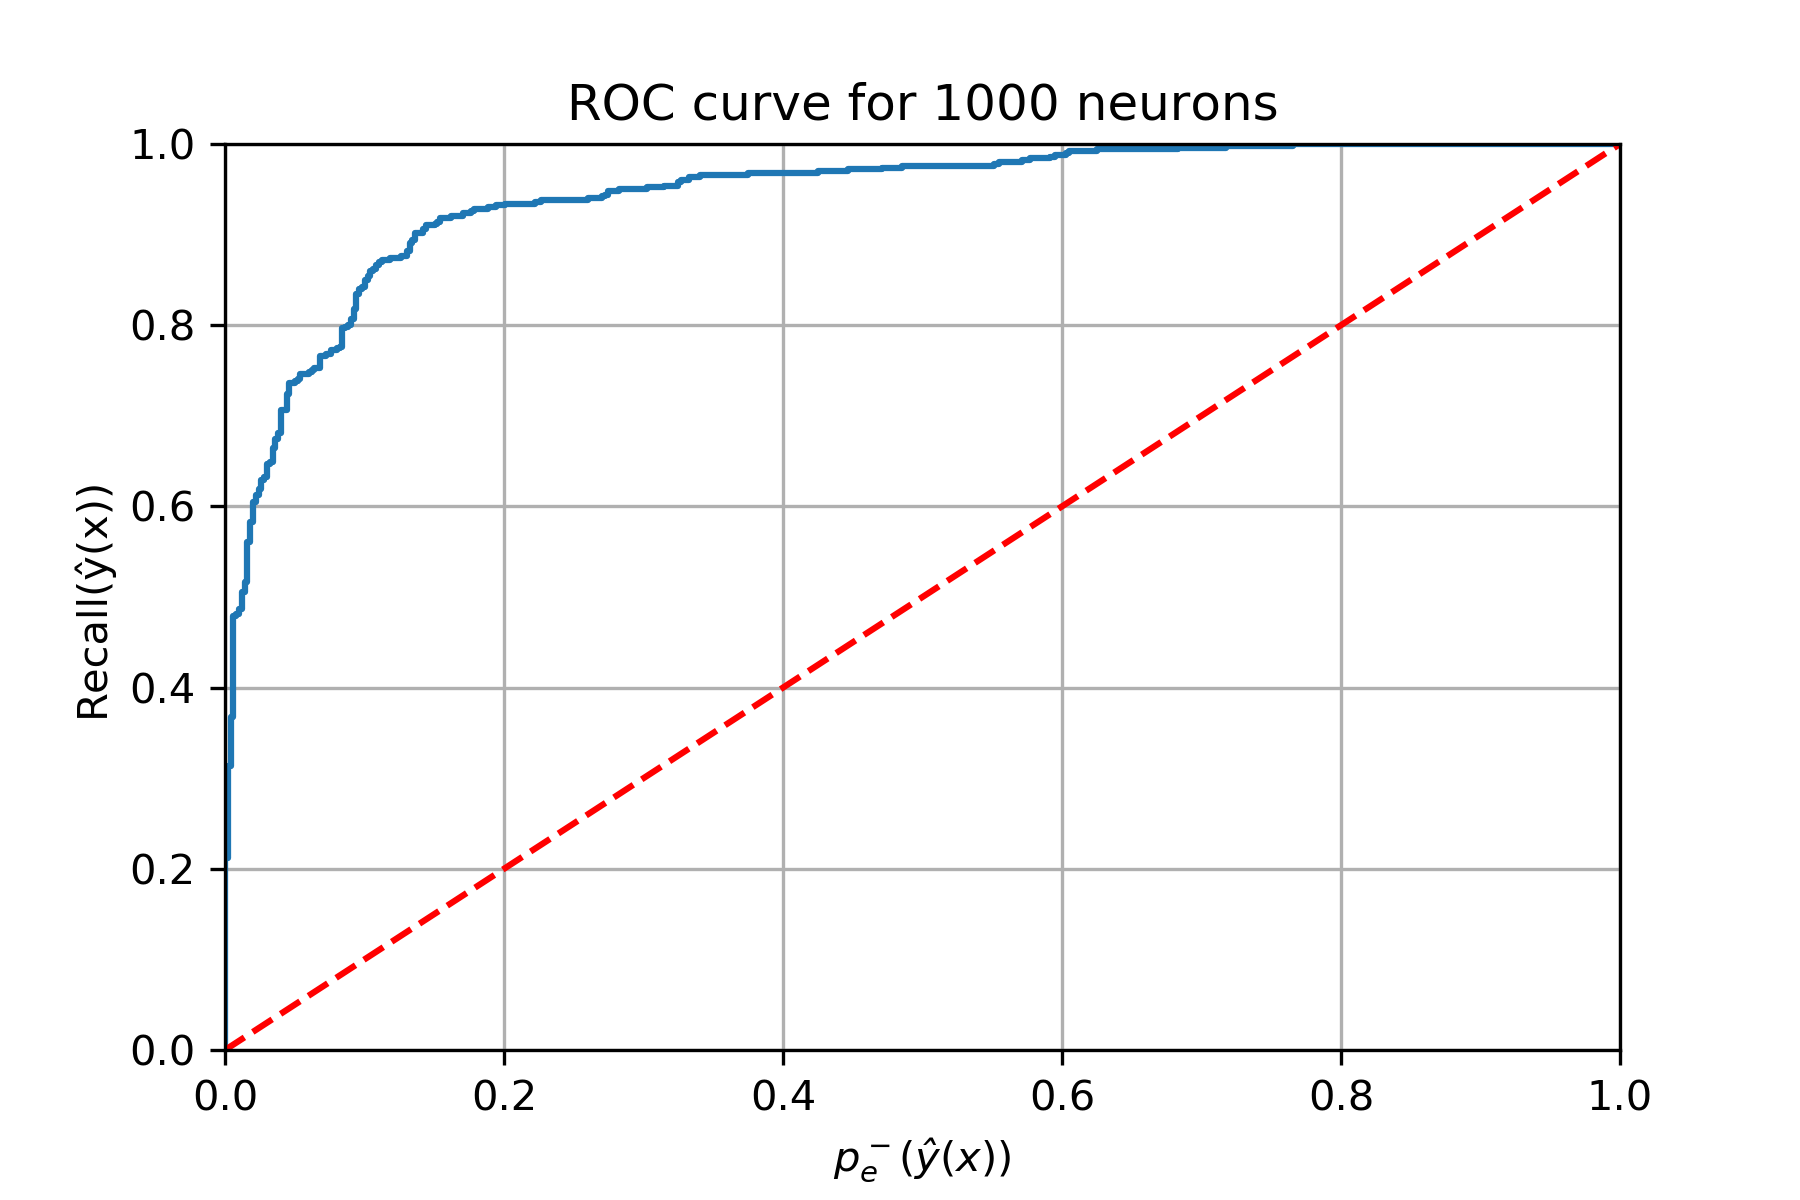
\includegraphics[width=3.85cm]{ROC_1000}
        \caption{1000 neurons}
        \label{fig:mlp-1000_roc}
    \end{subfigure}
    \hfill
    % 5000 neurons
    \begin{subfigure}{0.32\textwidth}
        \centering
        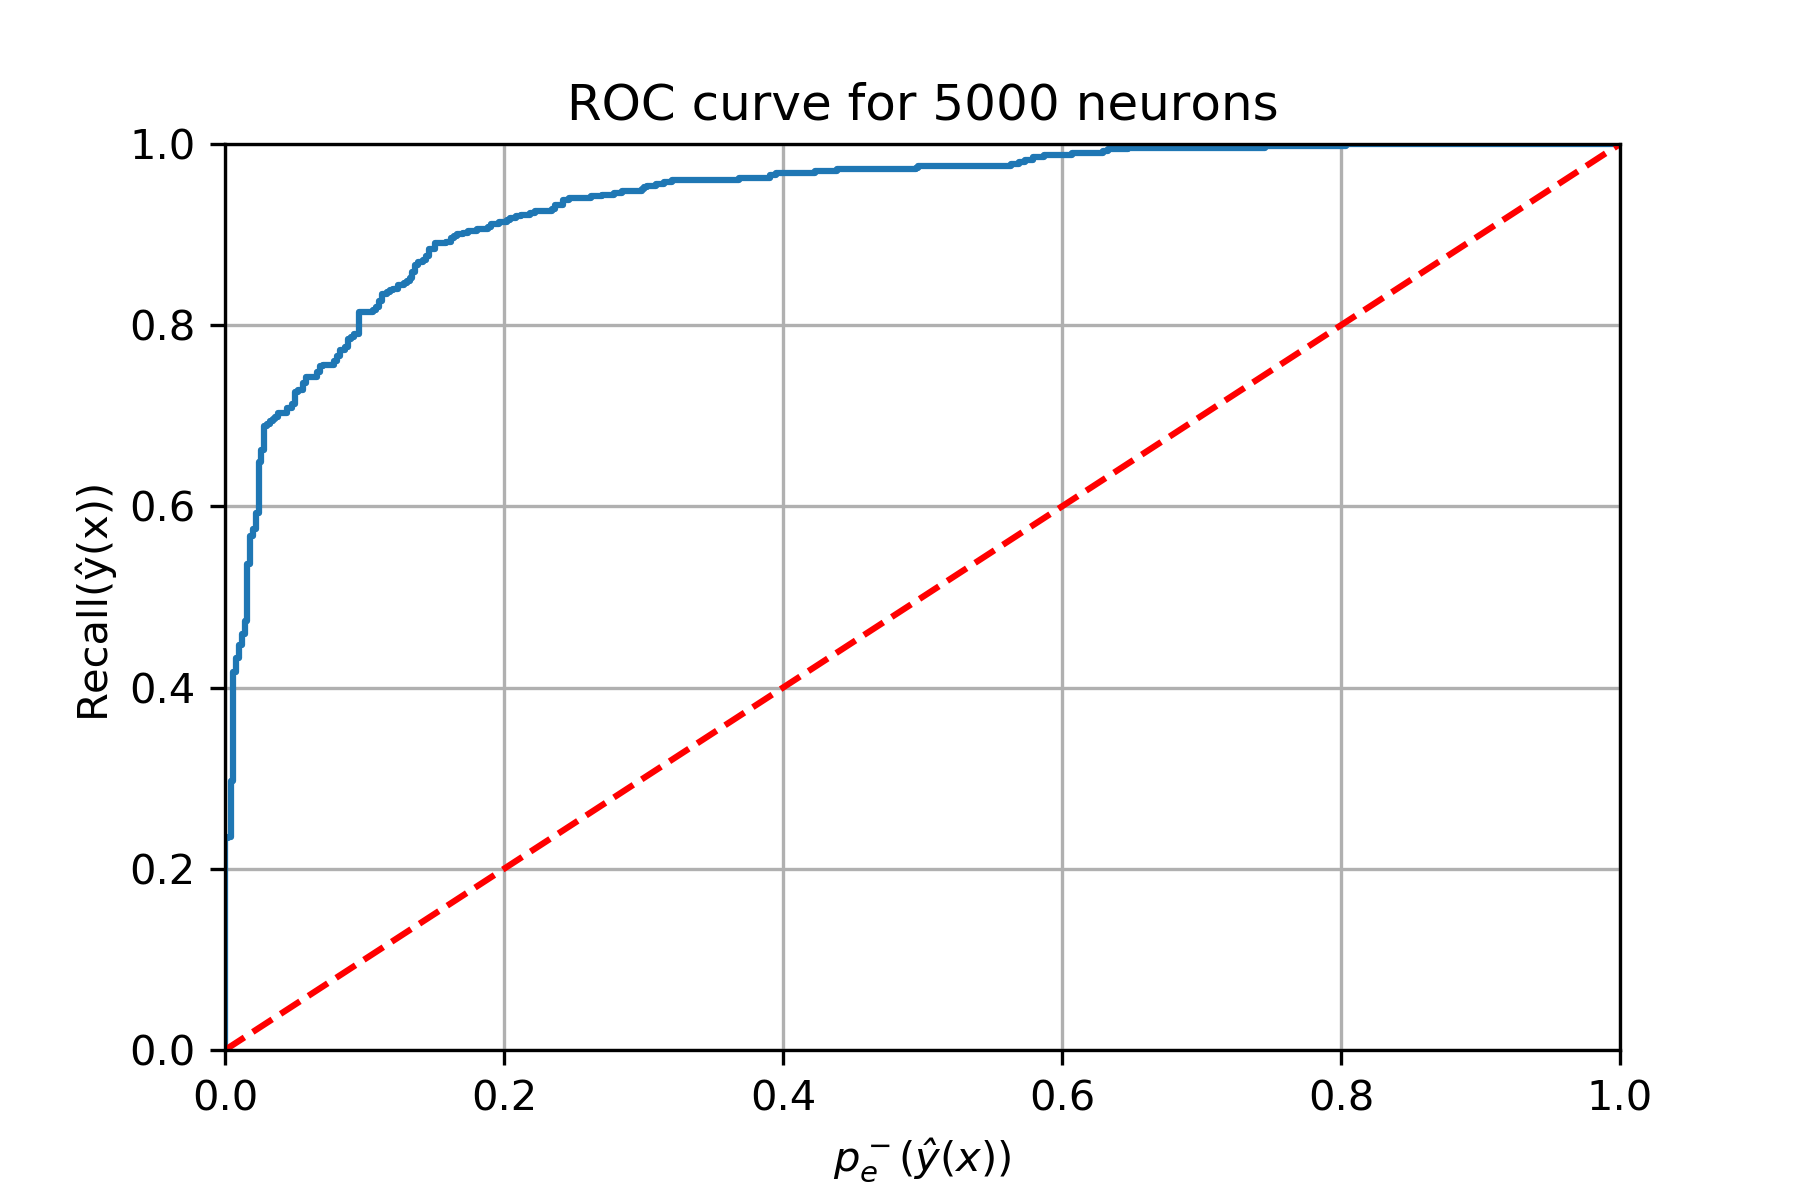
\includegraphics[width=3.85cm]{ROC_5000}
        \caption{5000 neurons}
        \label{fig:mlp-5000_roc}
    \end{subfigure}
    \hfill
    % caption and label
    \caption{ROC curves for MLP with different number of neurons}
    \label{fig:mlp-ROC_N_neurons}
\end{figure}
%-------------------------------------------------

\begin{figure}[H]
    \centering
    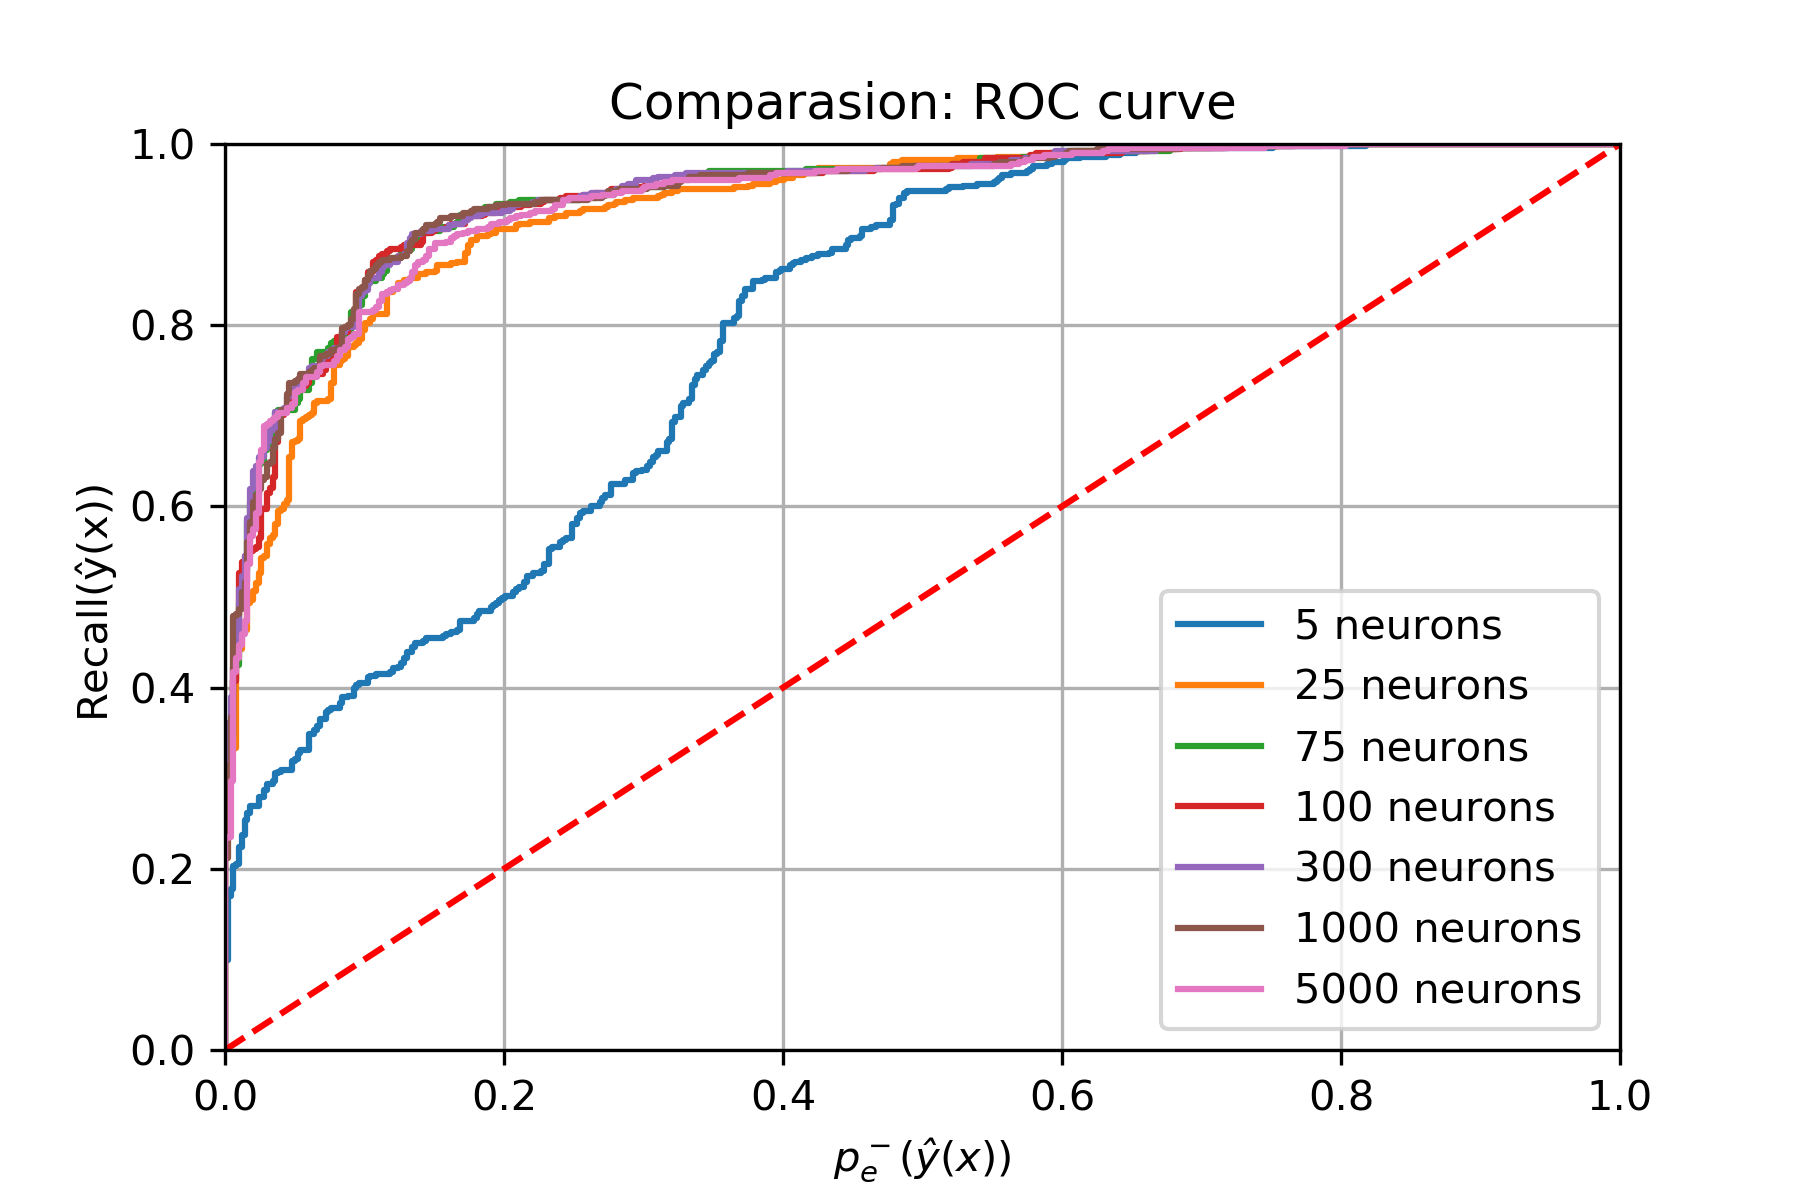
\includegraphics[width=12cm]{ROC_comparasion}
    \caption{}
    \label{fig:mlp-roc_comparasion}
\end{figure}

\newpage
%=================================================
\subsection{Support Vector Machine (SVM)}
%=================================================

\begin{figure}[H]
    \centering
    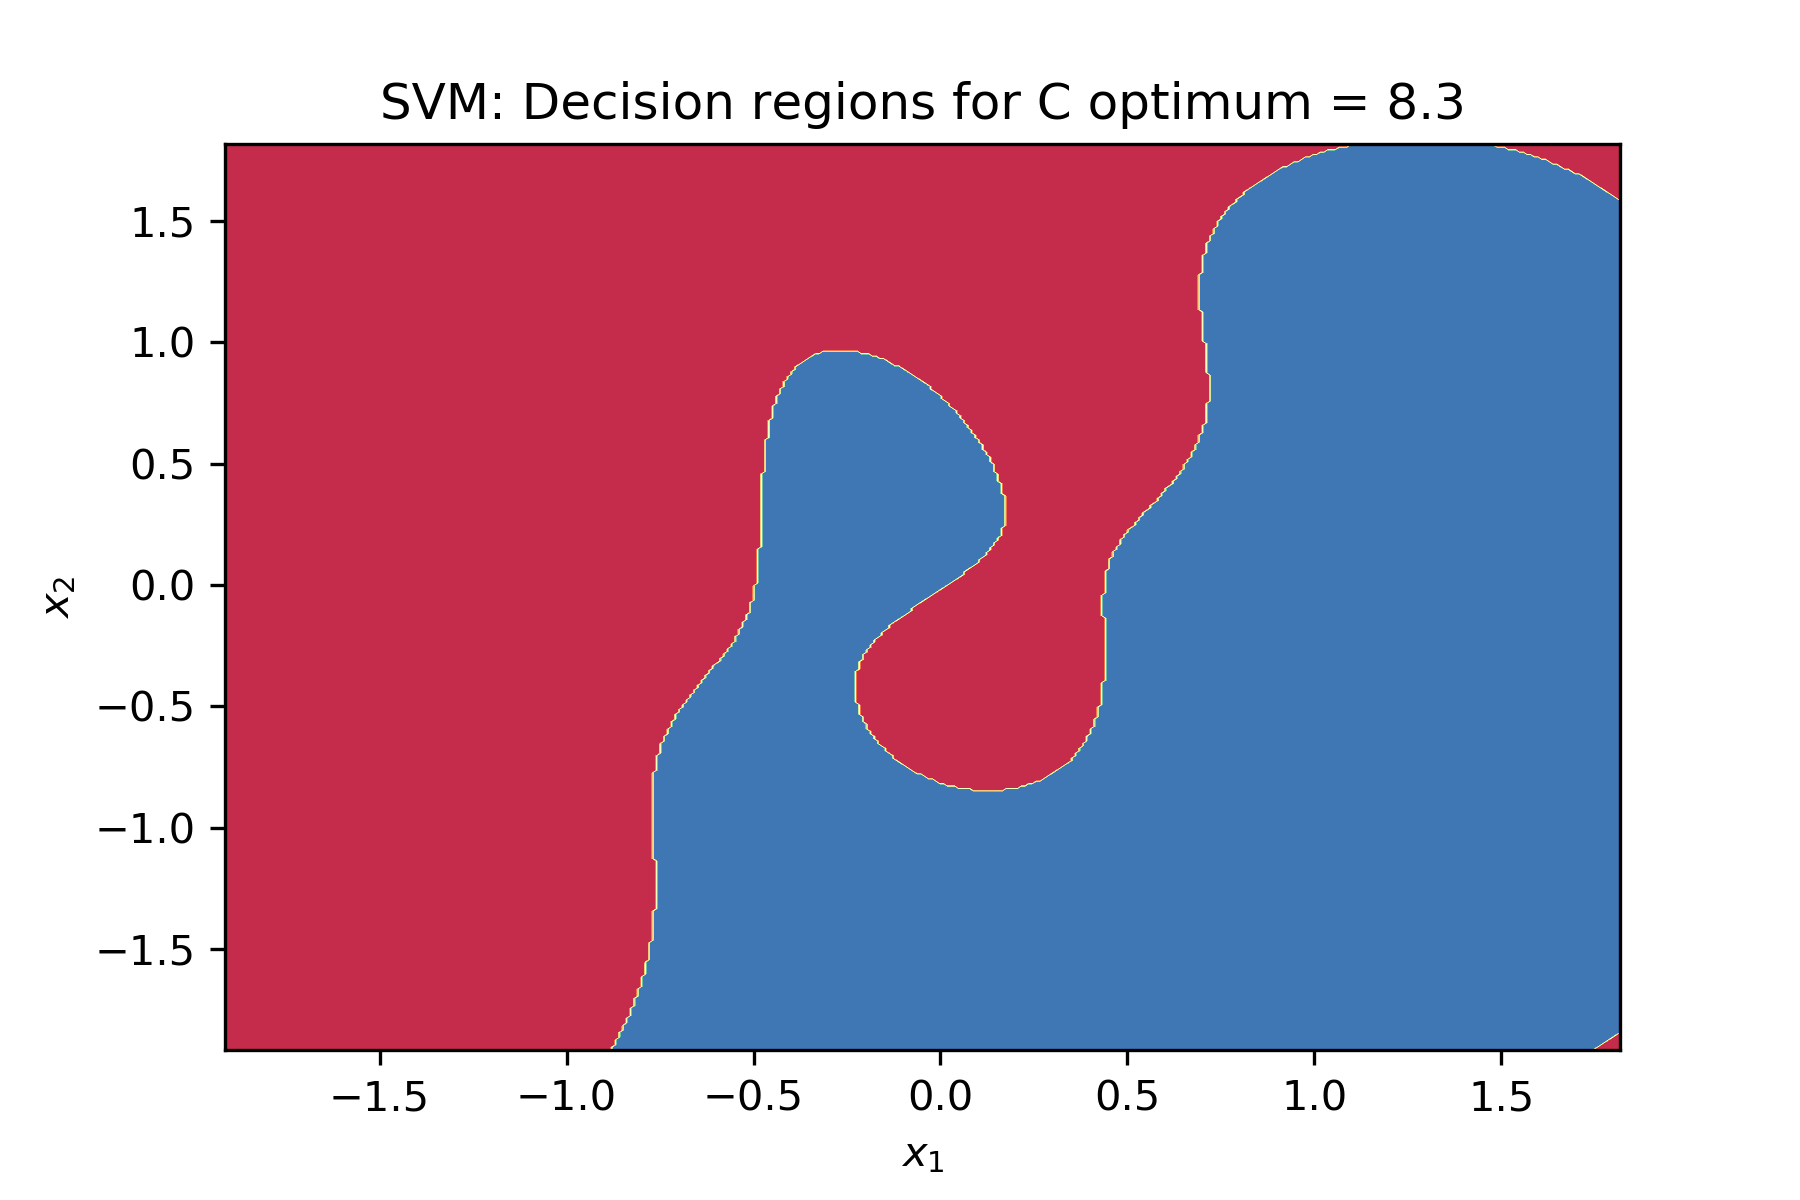
\includegraphics[width=12cm]{svm_decision_region}
    \caption{Decision regions}
    \label{fig:svm-decision_regions}
\end{figure}

\begin{figure}[H]
    \centering
    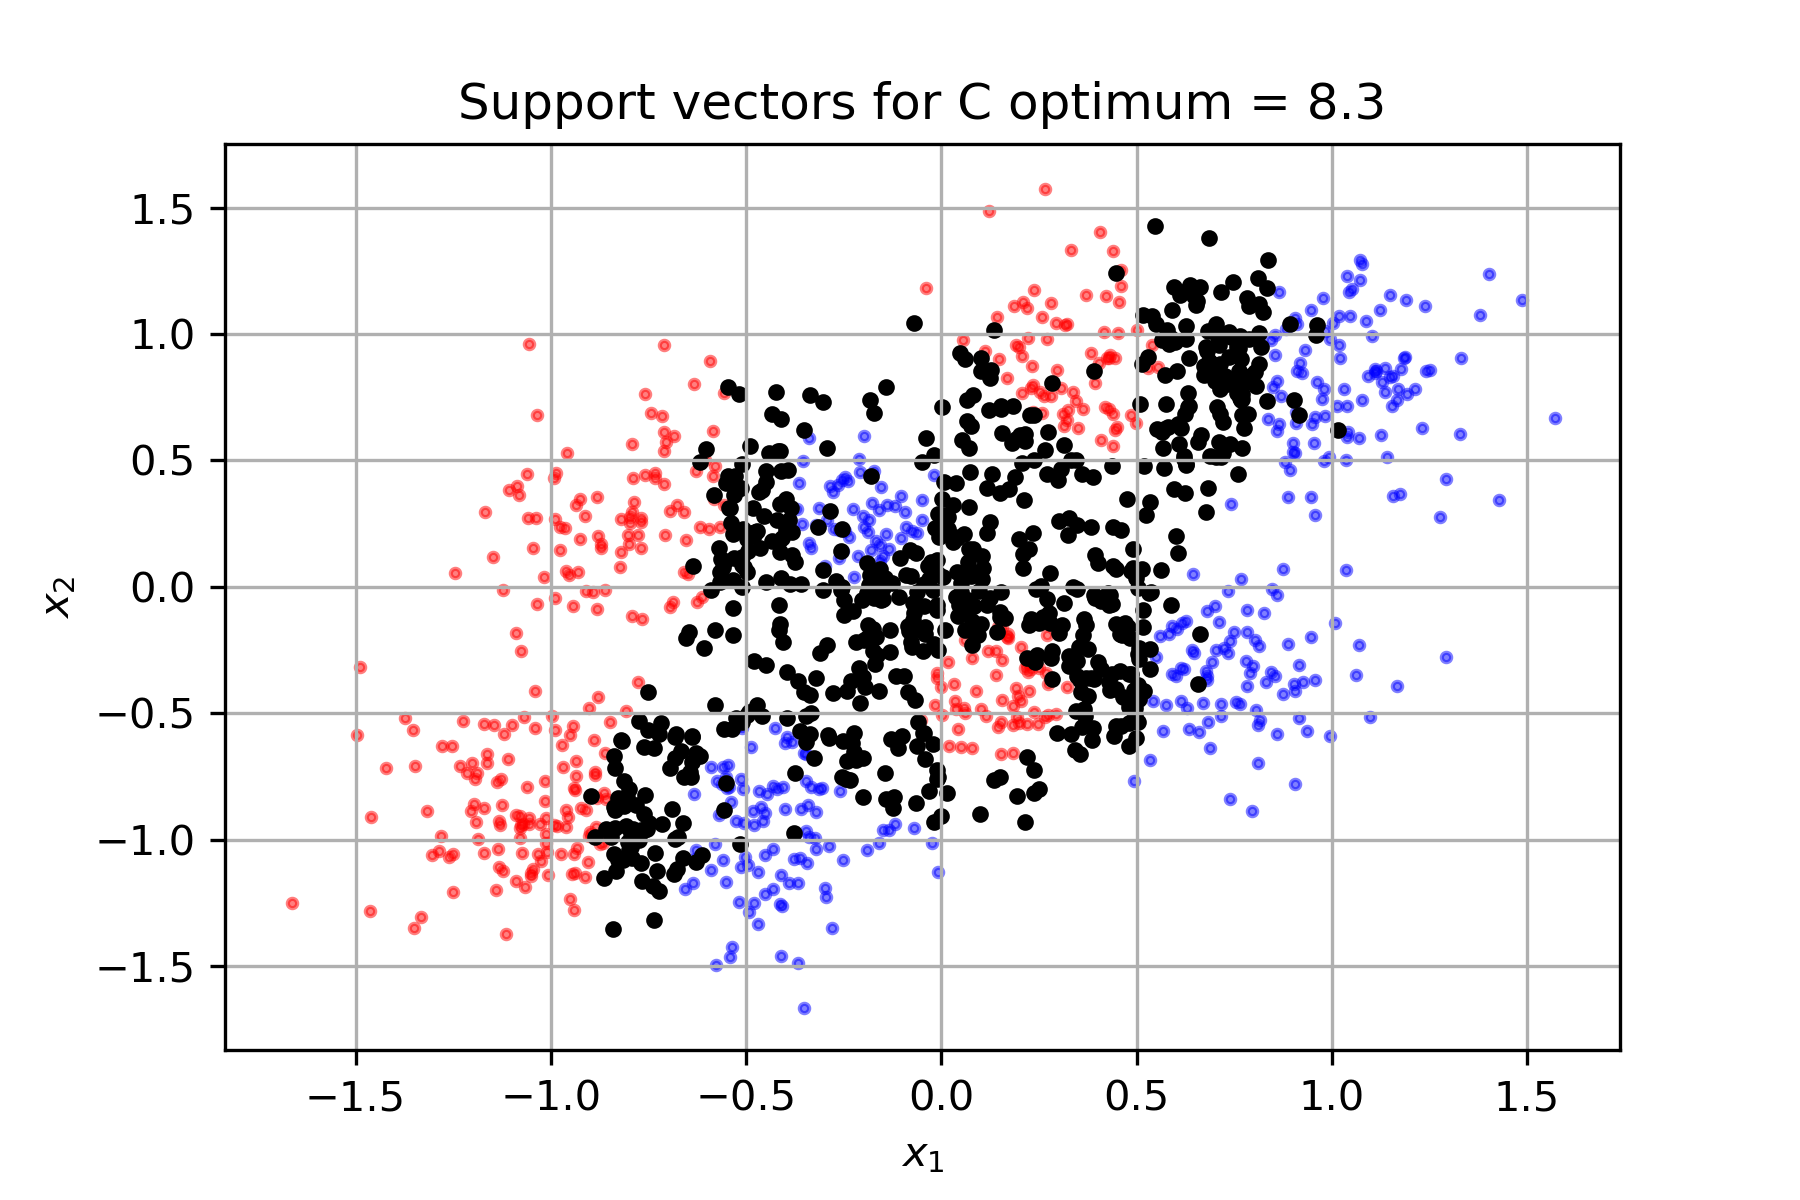
\includegraphics[width=12cm]{support_vectors}
    \caption{Support vectors}
    \label{fig:svm-support_vectors}
\end{figure}


%-------------------------------------------------
%\newpage
% decision regions for different values of hyperparameter C
% and the respective support vectors

\begin{figure}[H]
    %-----------------------------------
    \centering
    % decision regions (C = 0.1)
    \begin{subfigure}{0.45\textwidth}
        \centering
        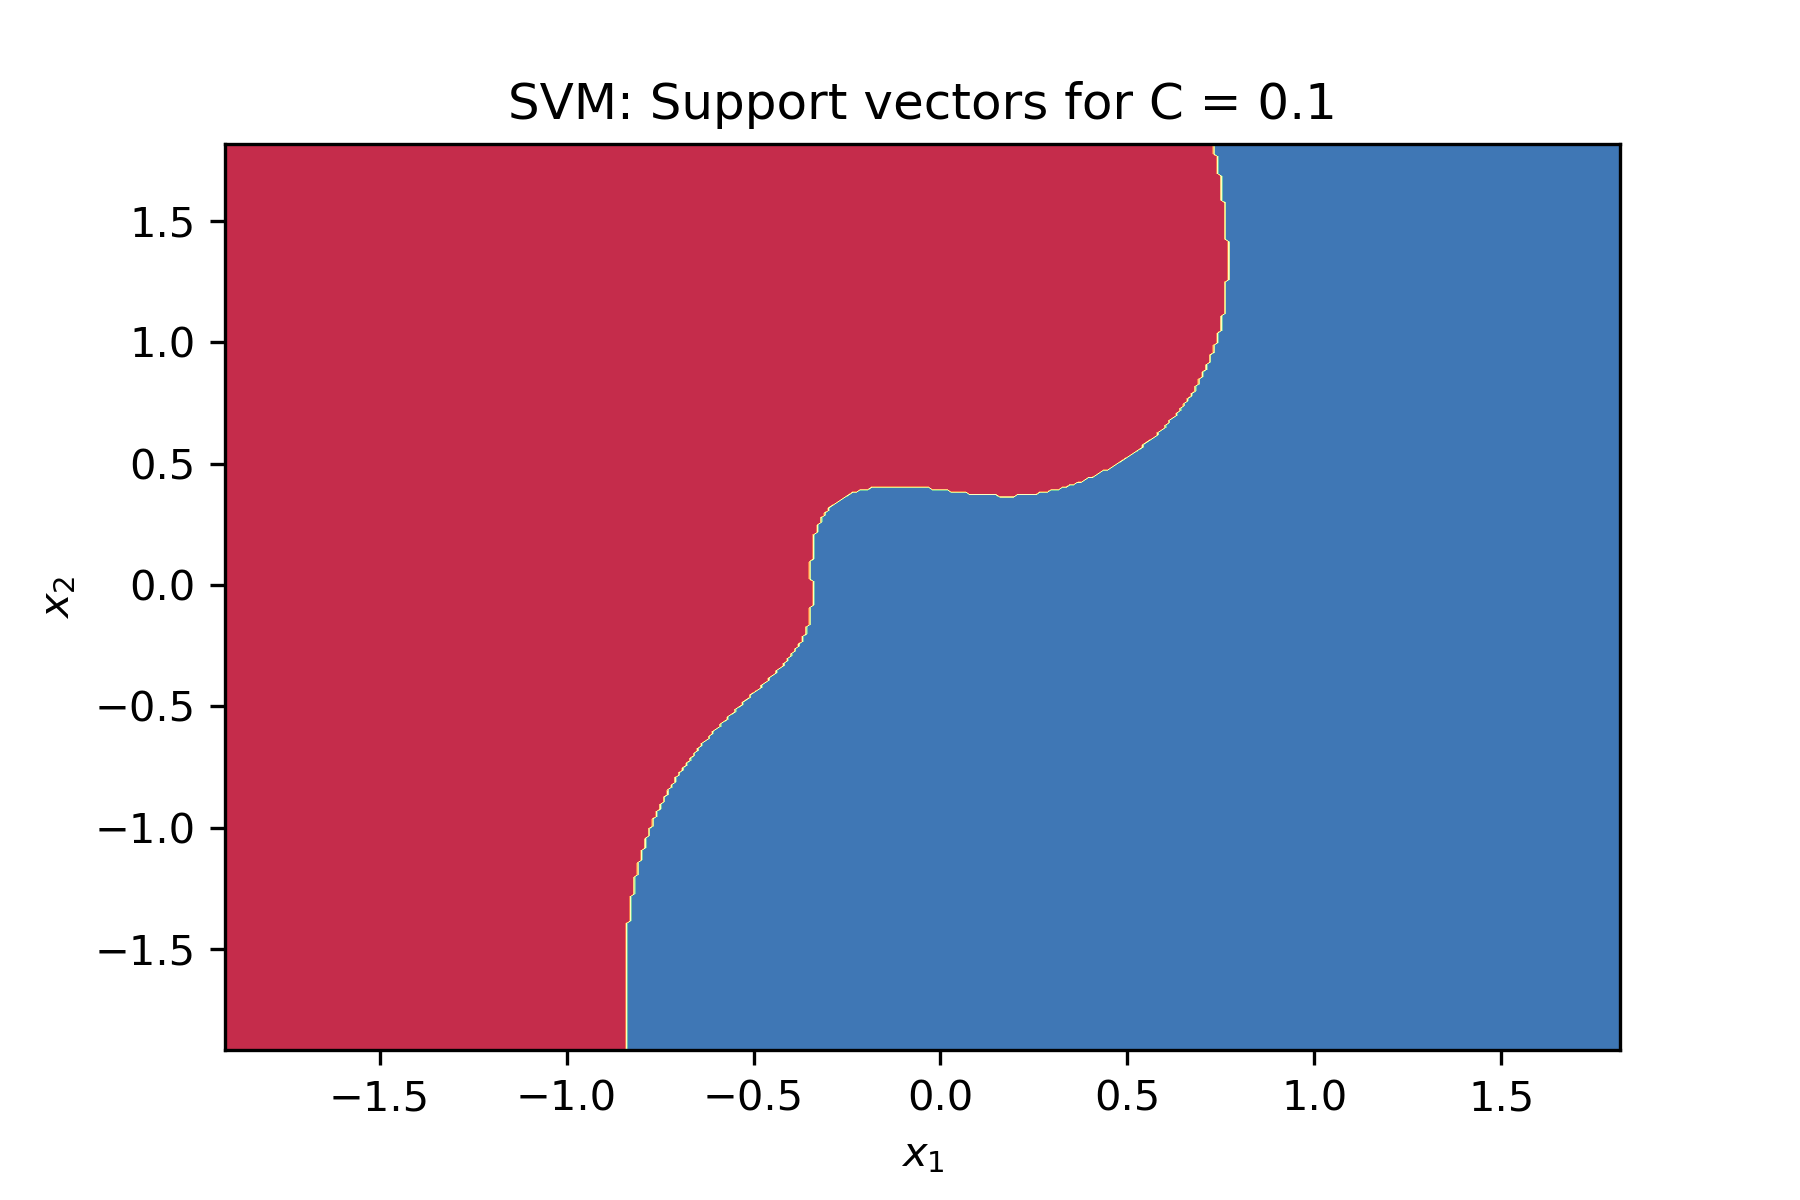
\includegraphics[width=7cm]{decision_region_C_0d1}
        \caption{Decision regions for C = 0.1}
        \label{fig:svm-decision_region_C_0d1}
    \end{subfigure}
    \hfill
    % support vectors (C = 0.1)
    \begin{subfigure}{0.45\textwidth}
        \centering
        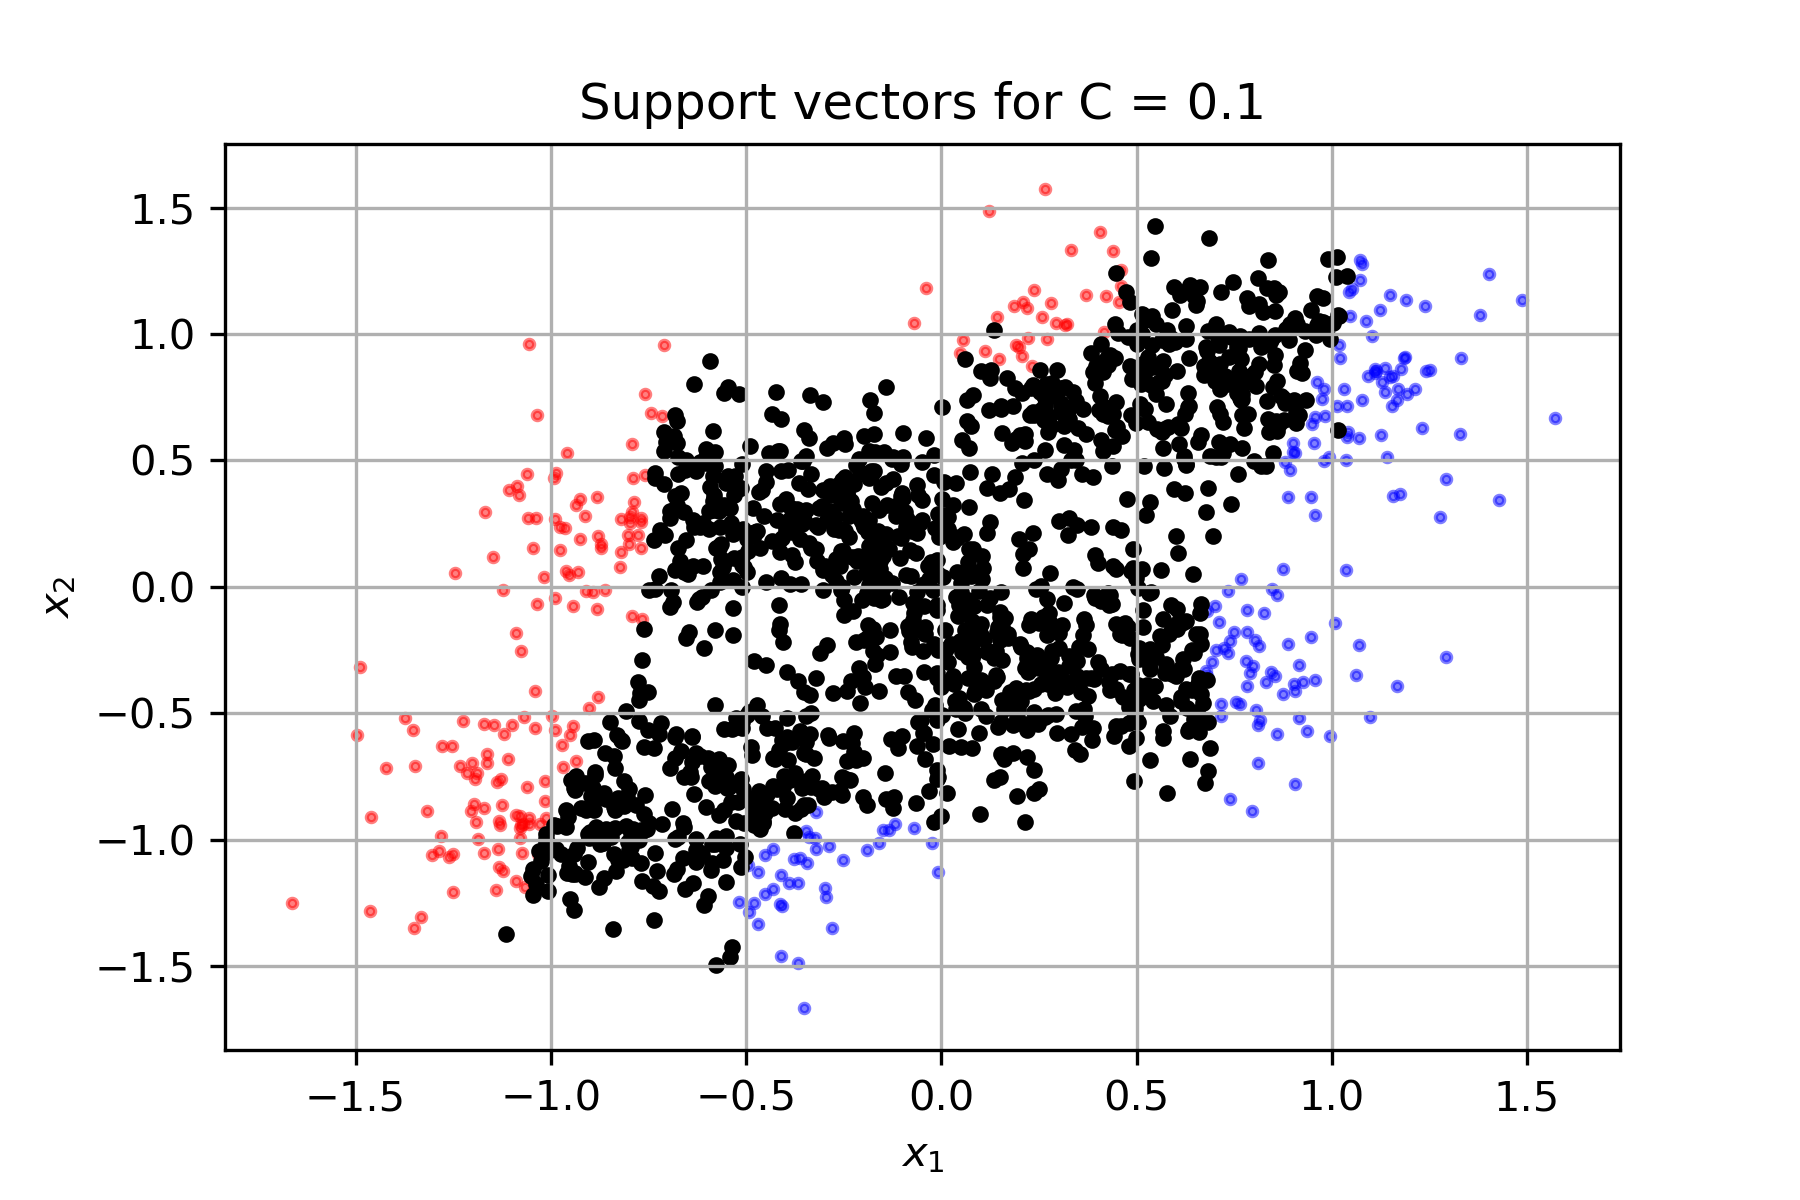
\includegraphics[width=7cm]{support_vectors_C_0d1}
        \caption{Support vectors for C = 0.1}
        \label{fig:svm-support_vectors_C_0d1}
    \end{subfigure}
    %-----------------------------------
    % decision regions (C = 1.0)
    \begin{subfigure}{0.45\textwidth}
        \centering
        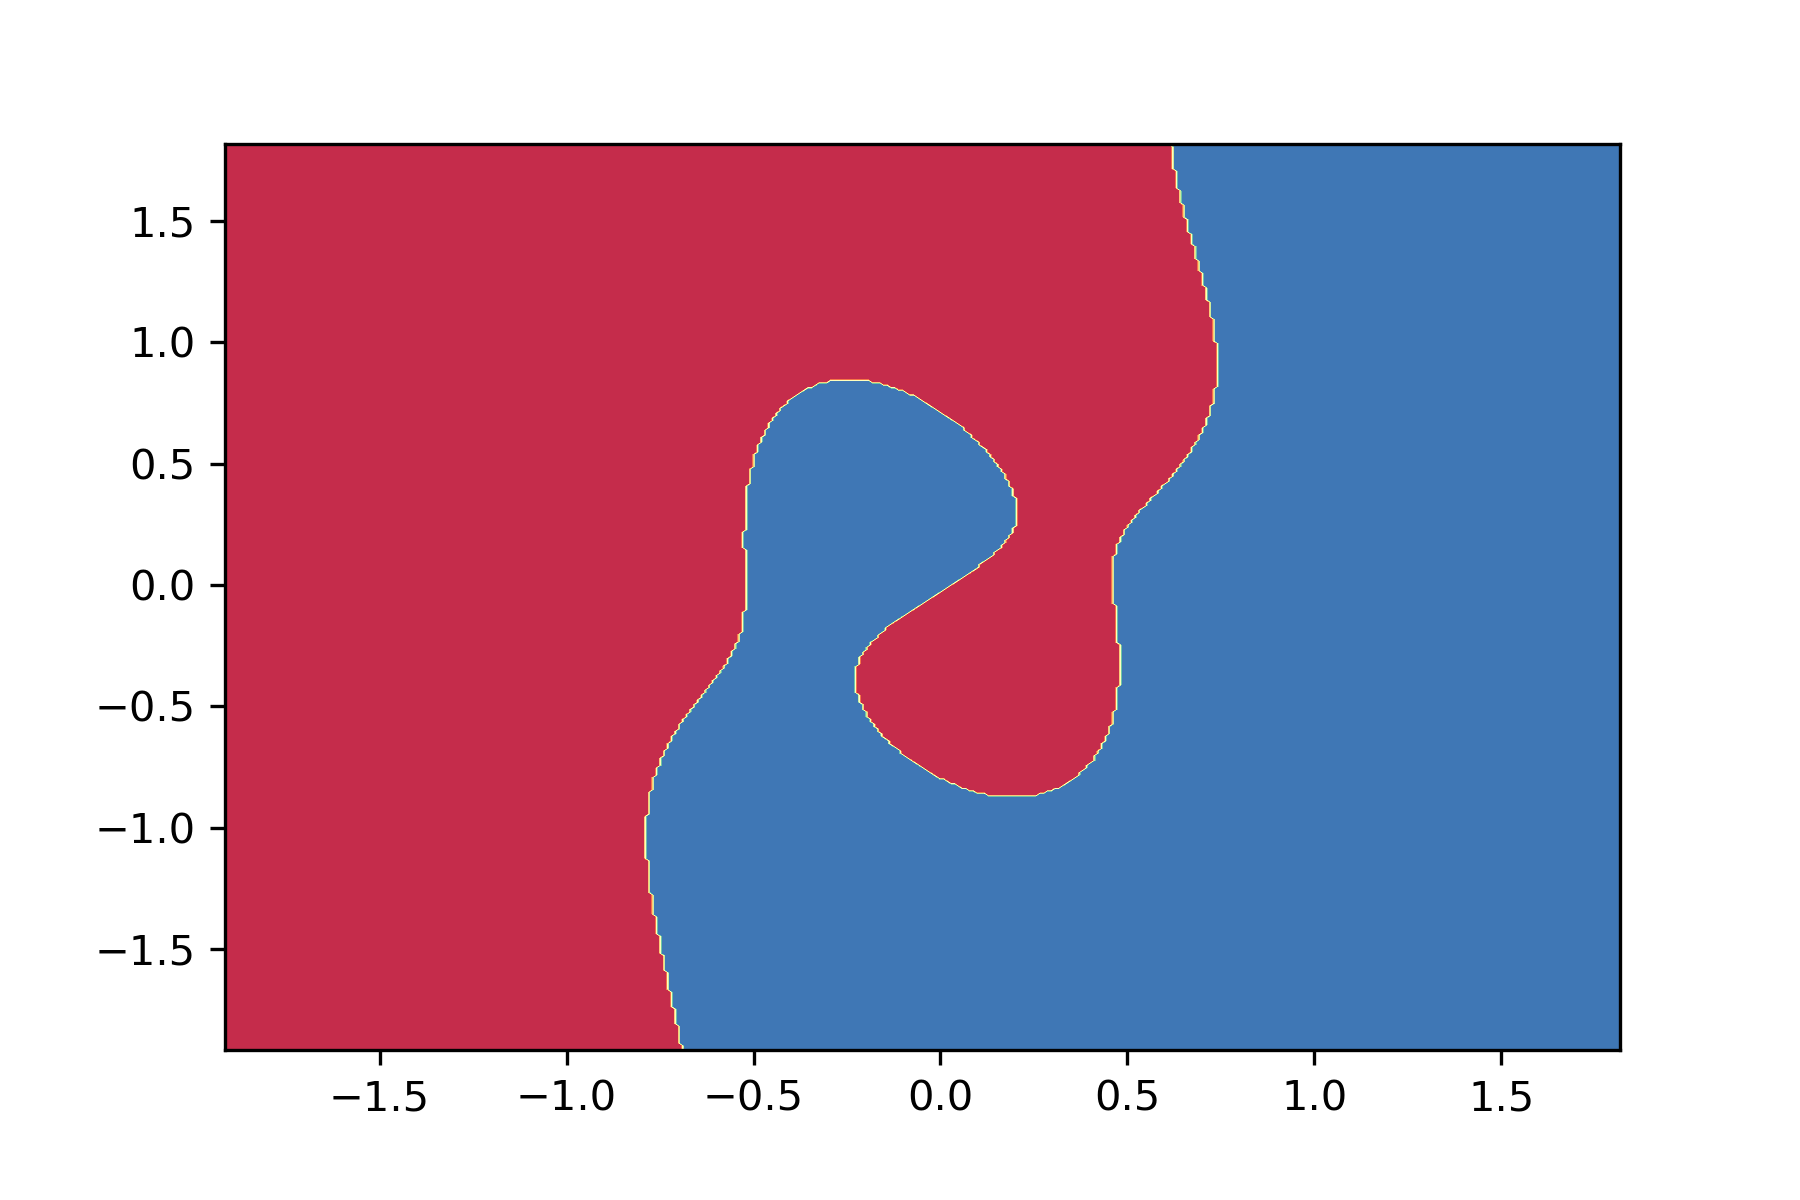
\includegraphics[width=7cm]{decision_region_C_1}
        \caption{Decision regions for C = 1.0}
        \label{fig:svm-decision_region_C_1}
    \end{subfigure}
    \hfill
    % support vectors (C = 1.0)
    \begin{subfigure}{0.45\textwidth}
        \centering
        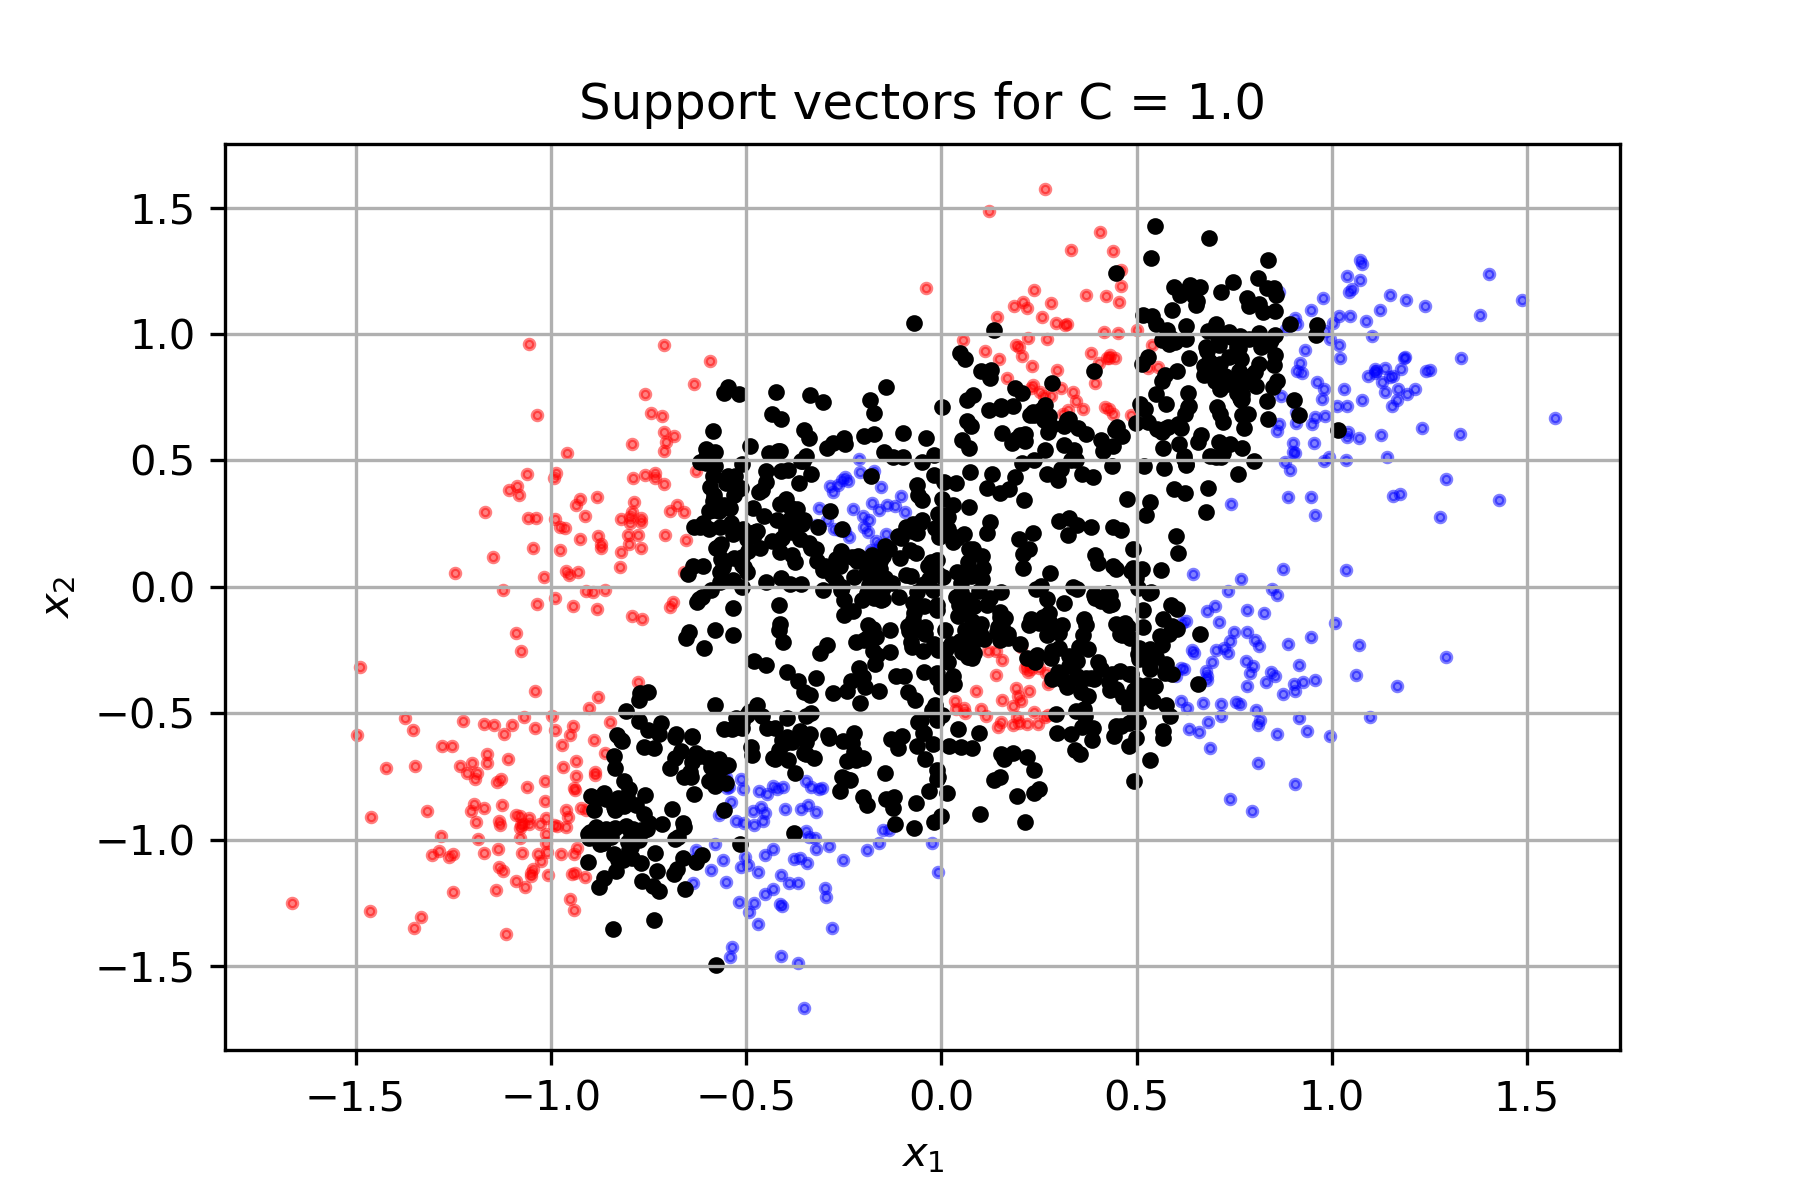
\includegraphics[width=7cm]{support_vectors_C_1}
        \caption{Support vectors for C = 1.0}
        \label{fig:svm-support_vectors_C_1}
    \end{subfigure}
    %-----------------------------------
    % decision regions (C = 20)
    \begin{subfigure}{0.45\textwidth}
        \centering
        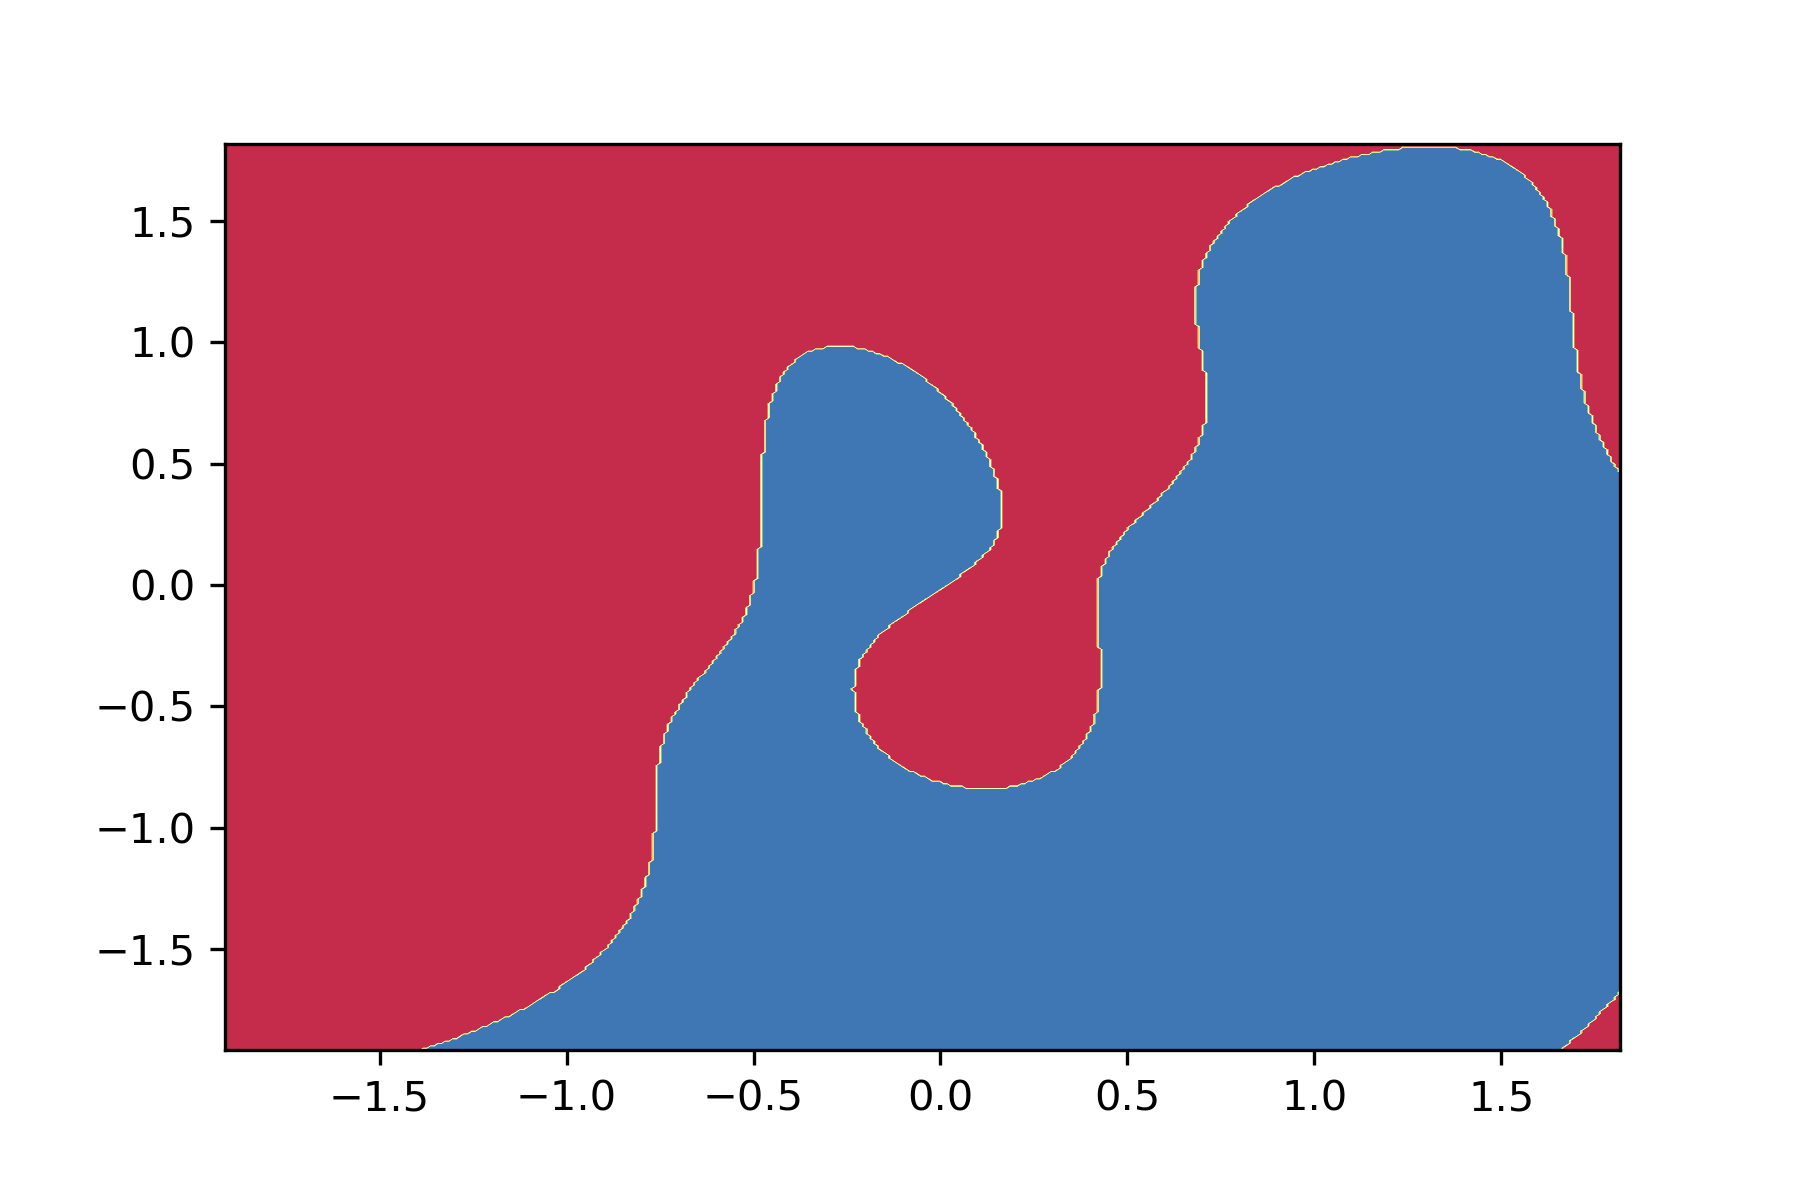
\includegraphics[width=7cm]{decision_region_C_20}
        \caption{Decision regions for C = 20}
        \label{fig:svm-decision_region_C_20}
    \end{subfigure}
    \hfill
    % support vectors (C = 20)
    \begin{subfigure}{0.45\textwidth}
        \centering
        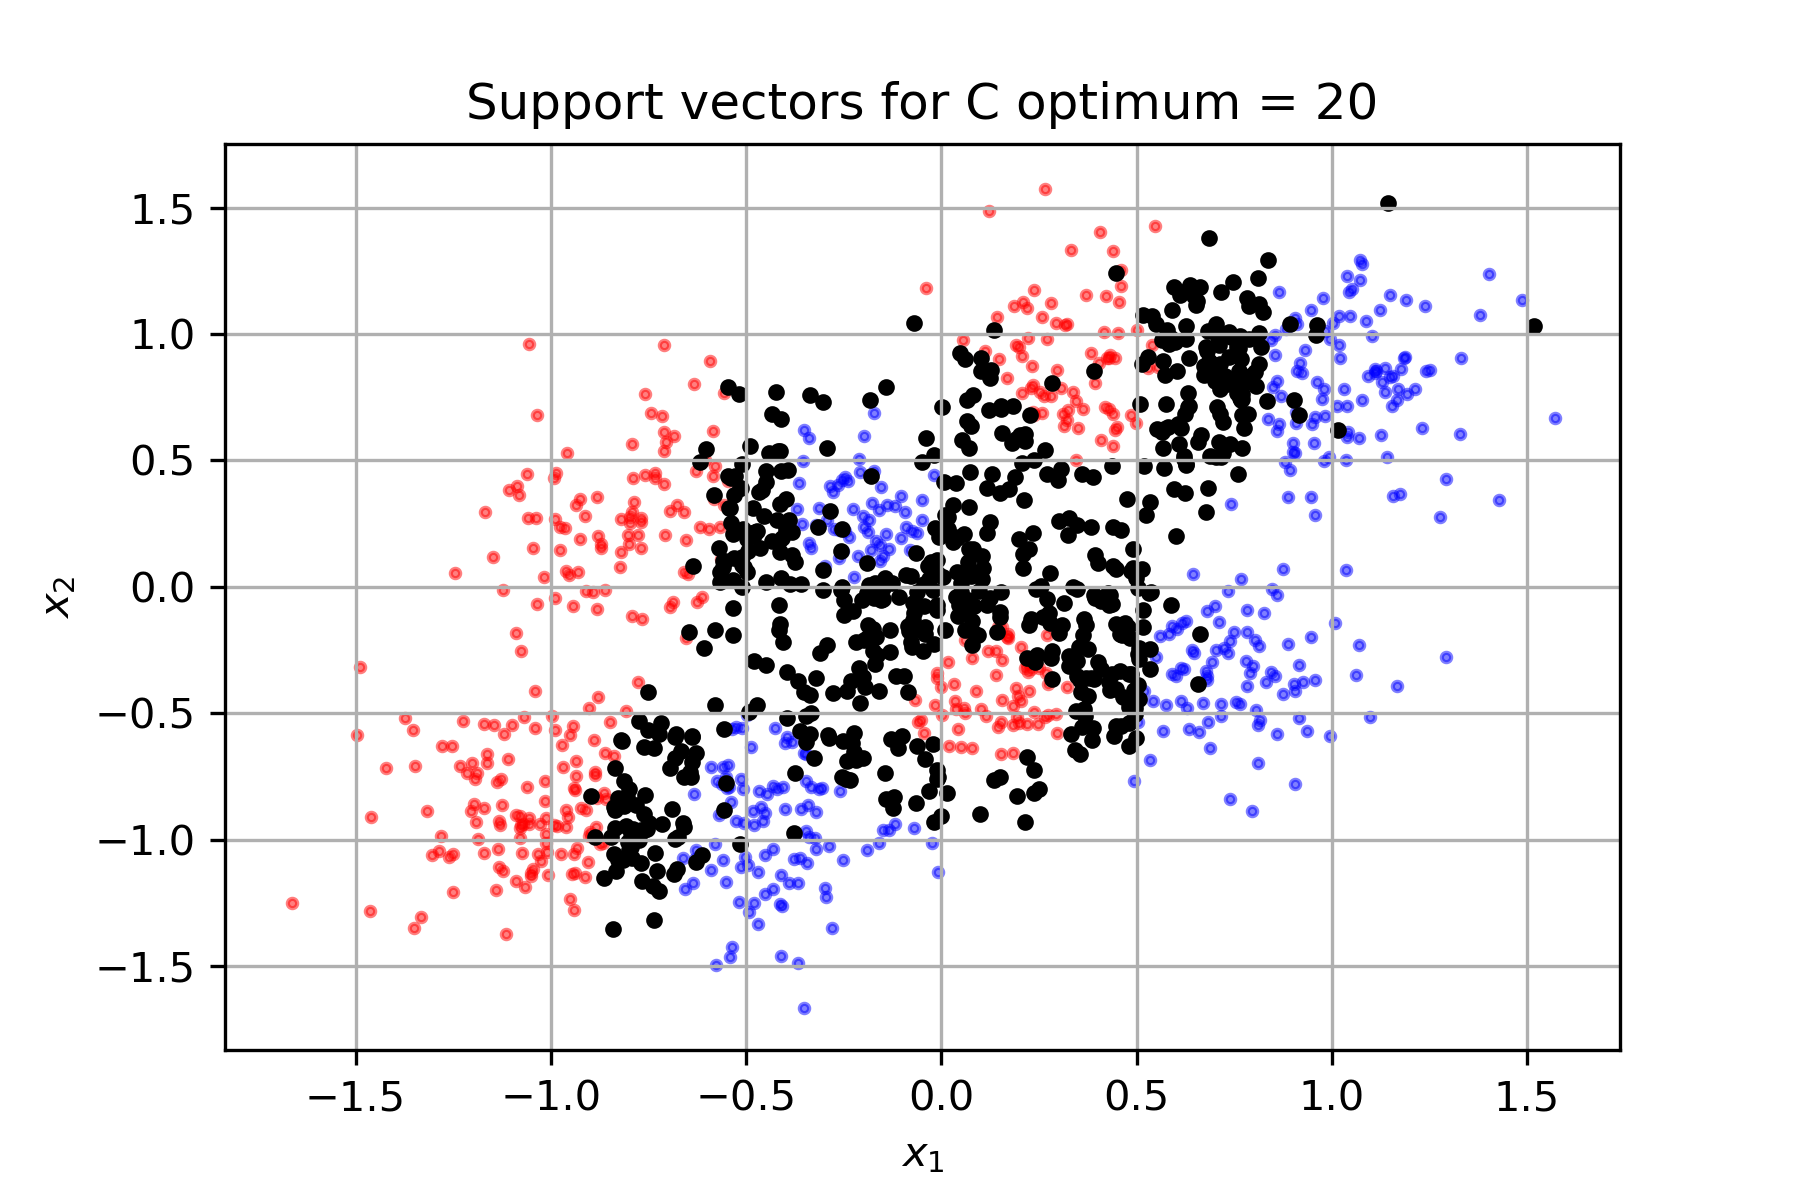
\includegraphics[width=7cm]{support_vectors_C_20}
        \caption{Support vectors for C = 20}
        \label{fig:svm-support_vectors_C_20}
    \end{subfigure}
    %-----------------------------------
    % decision regions (C = 1000)
    \begin{subfigure}{0.45\textwidth}
        \centering
        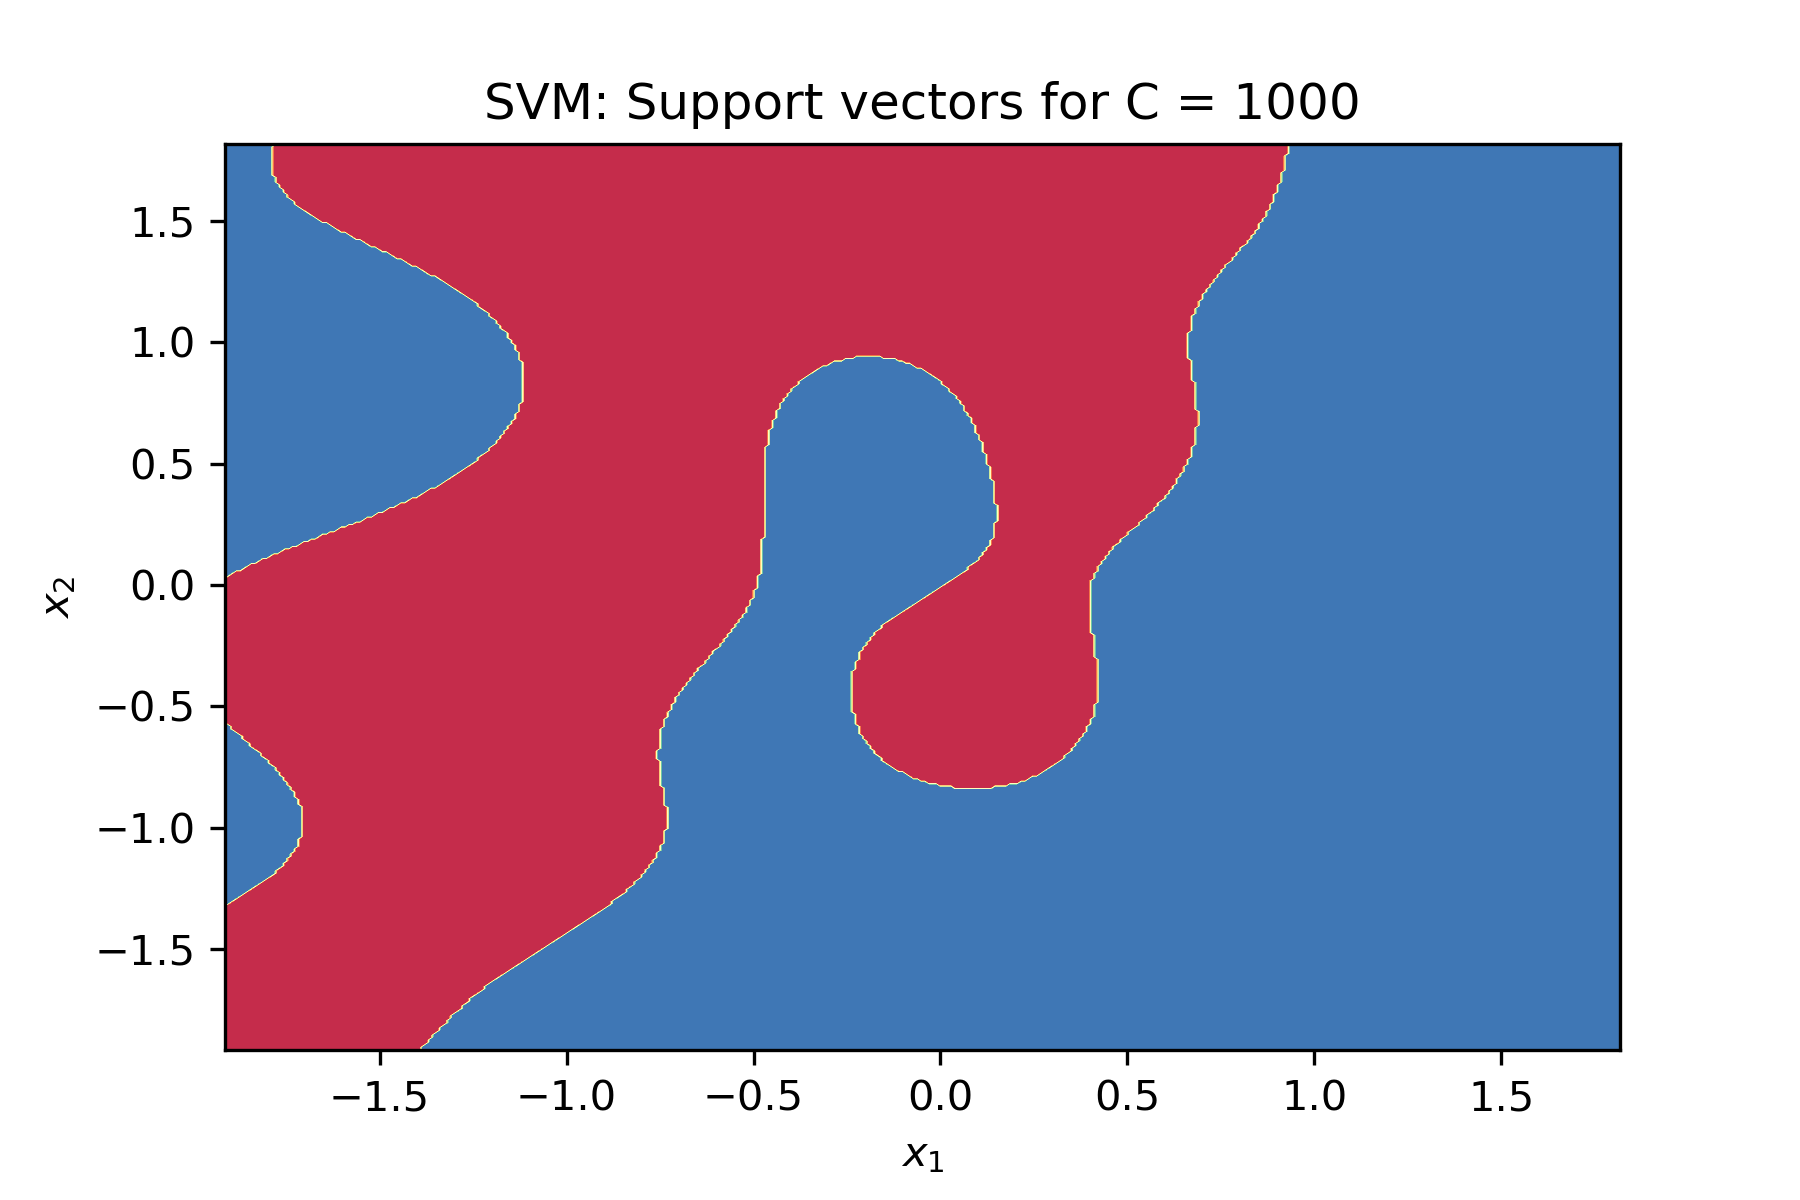
\includegraphics[width=7cm]{decision_region_C_1000}
        \caption{Decision regions for C = 1000}
        \label{fig:svm-decision_region_C_1000}
    \end{subfigure}
    \hfill
    % support vectors (C = 1000)
    \begin{subfigure}{0.45\textwidth}
        \centering
        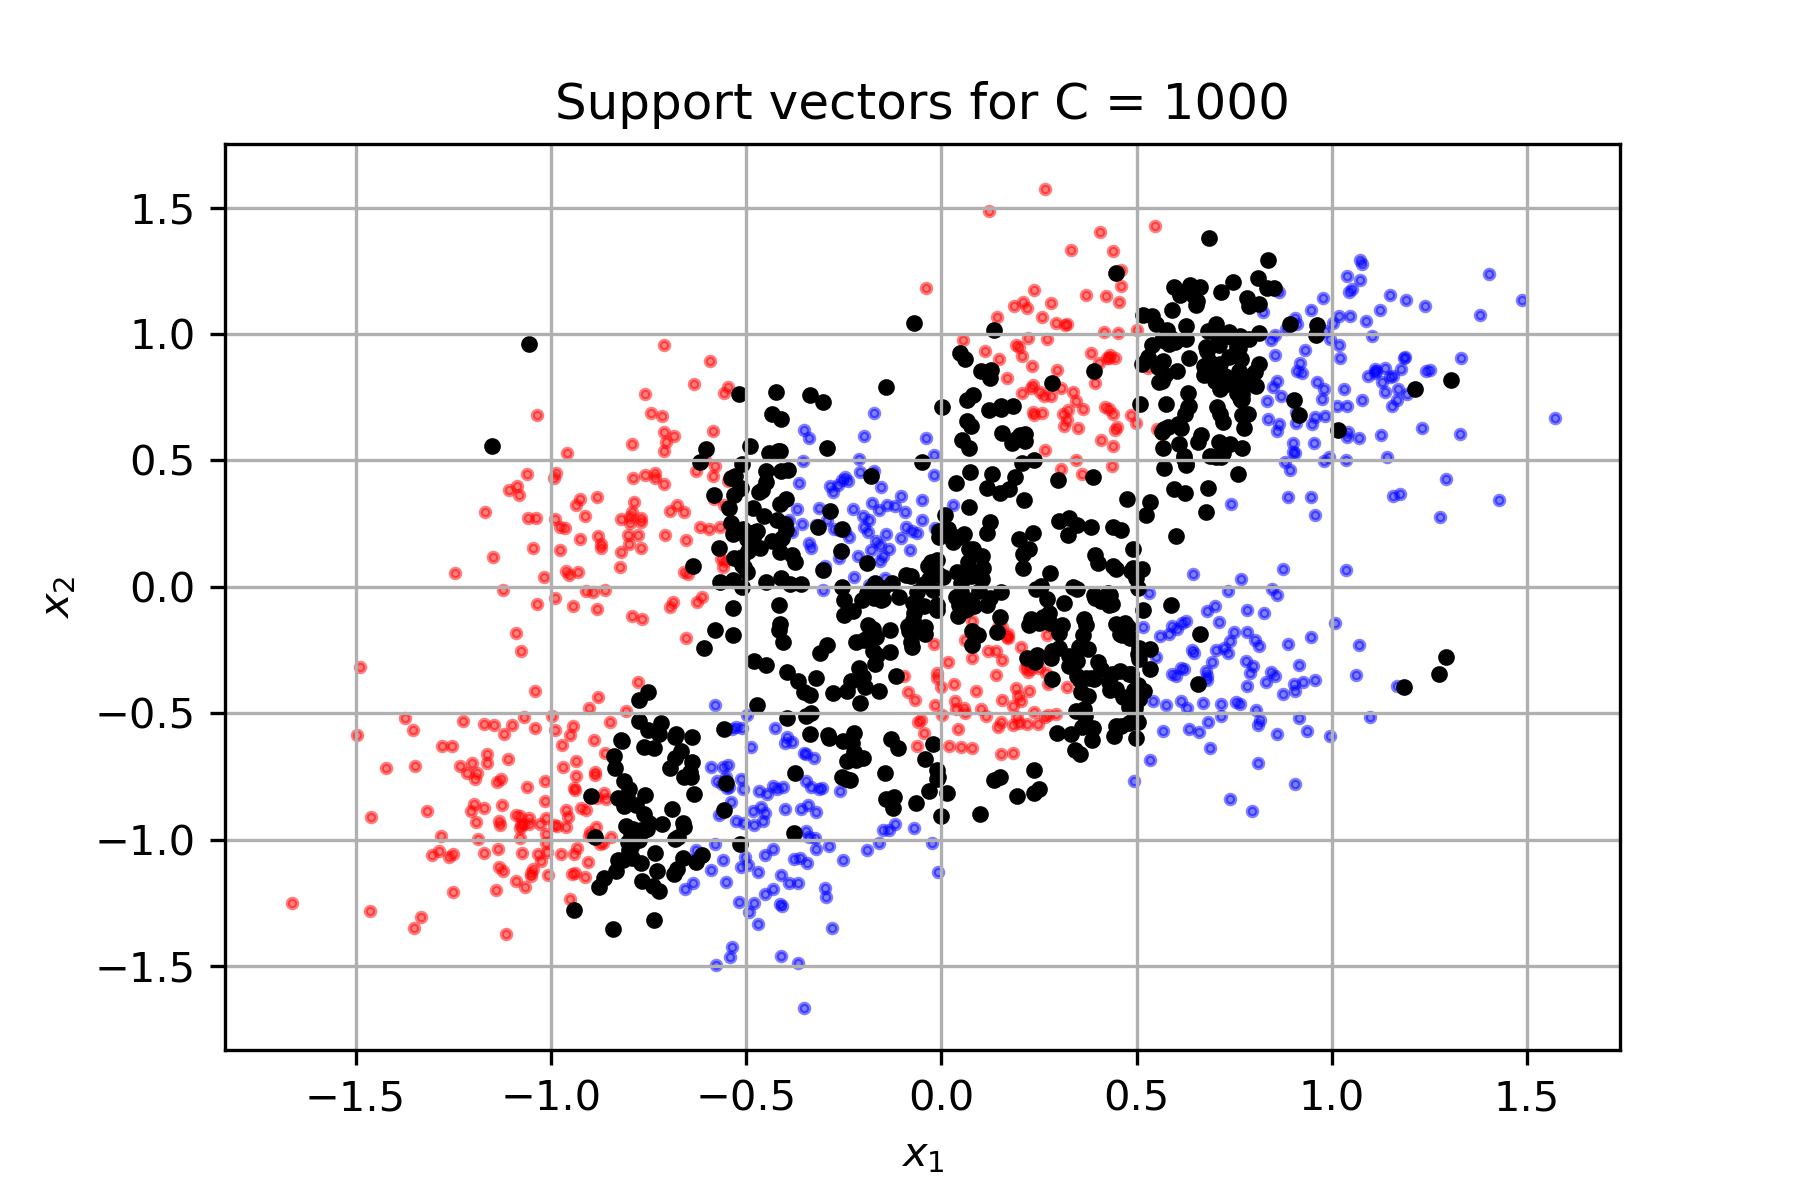
\includegraphics[width=7cm]{support_vectors_C_1000}
        \caption{Support vectors for C = 1000}
        \label{fig:svm-support_vectors_C_1000}
    \end{subfigure}
    %-----------------------------------
    % caption and label
    \caption{Decision regions and respective support vectors for different values of hyperparameter C}
    \label{fig:svm-decision_regions_support_vectos_C}
\end{figure}
%-------------------------------------------------




%-------------------------------------------------
%\newpage
% decision regions for different values of hyperparameter gamma
% and the respective support vectors

\begin{figure}[H]
    %-----------------------------------
    \centering
    % decision regions (gamma = 0.1)
    \begin{subfigure}{0.45\textwidth}
        \centering
        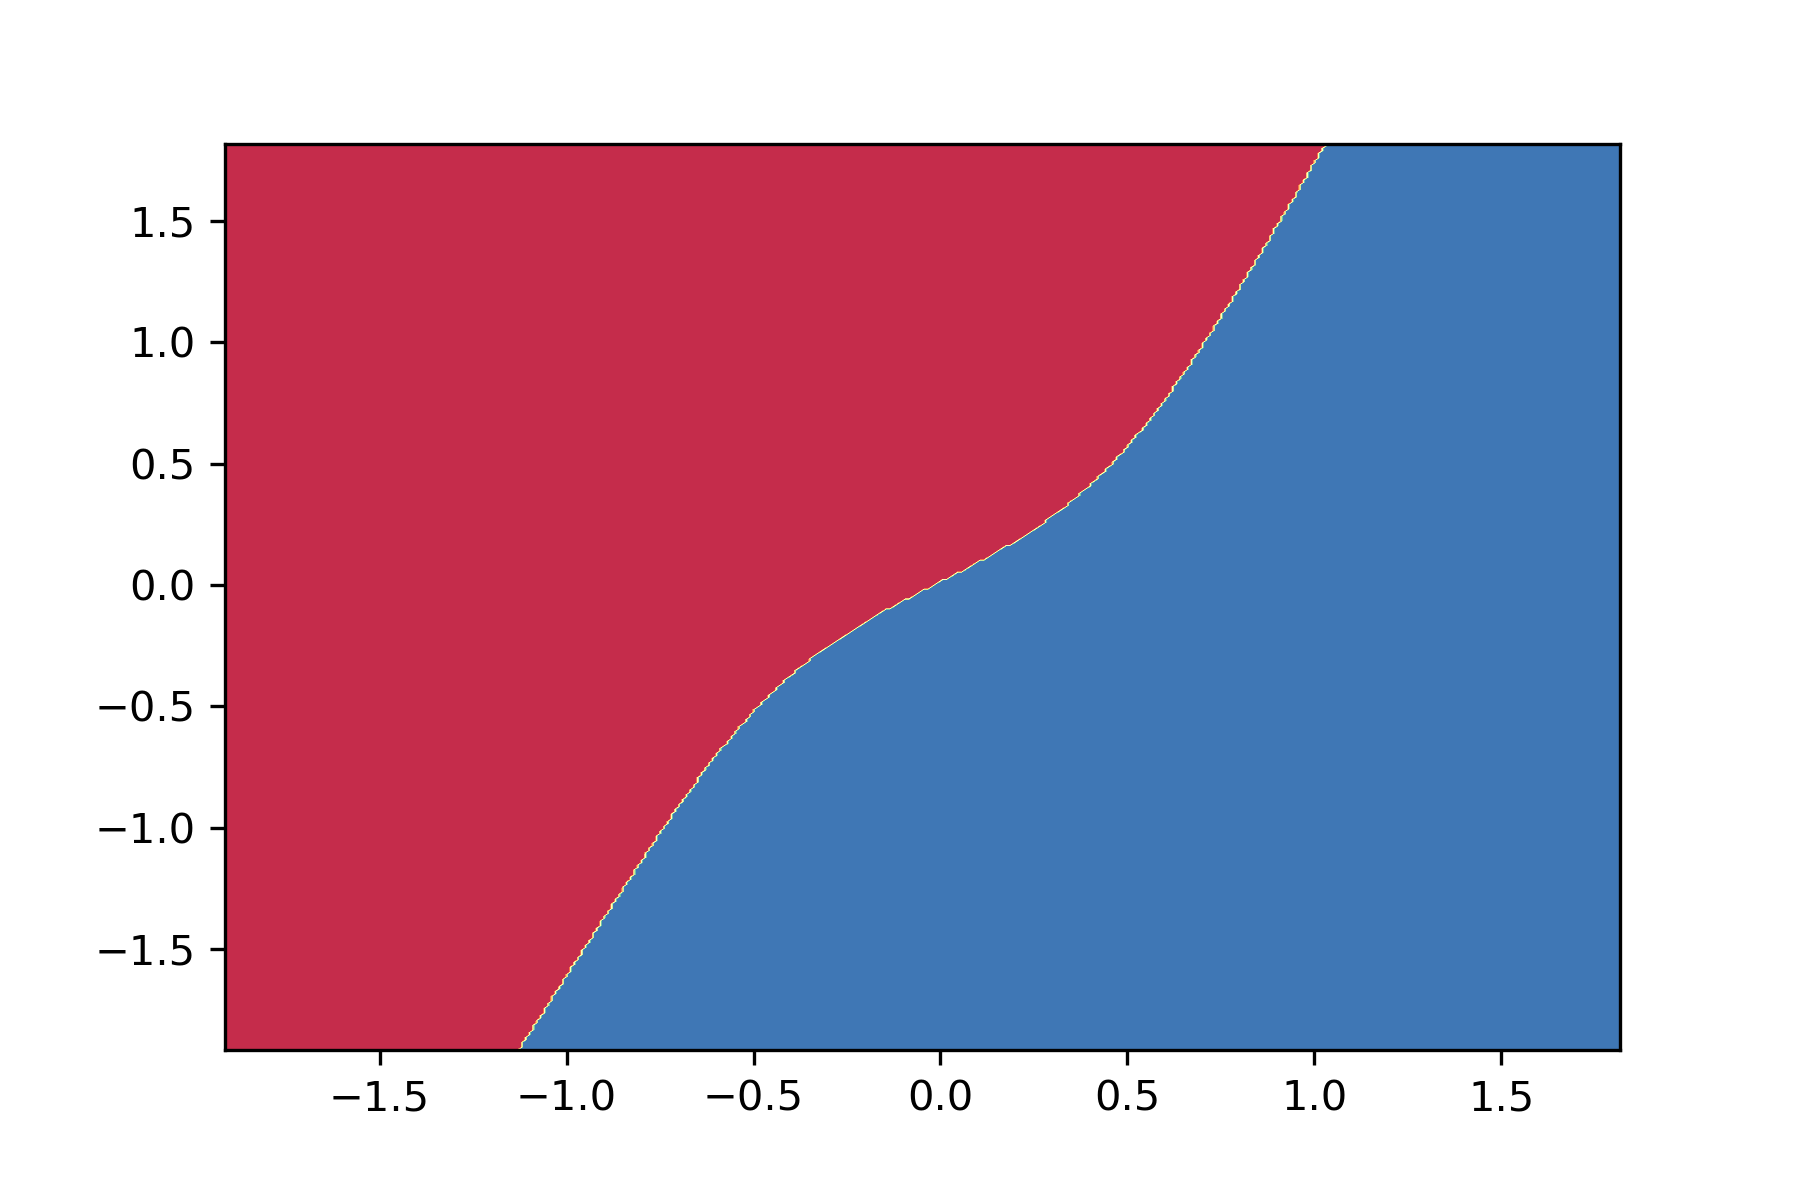
\includegraphics[width=7cm]{decision_region_gamma_0d1}
        \caption{Decision regions for gamma = 0.1}
        \label{fig:svm-decision_region_gamma_0d1}
    \end{subfigure}
    \hfill
    % support vectors (gamma = 0.1)
    \begin{subfigure}{0.45\textwidth}
        \centering
        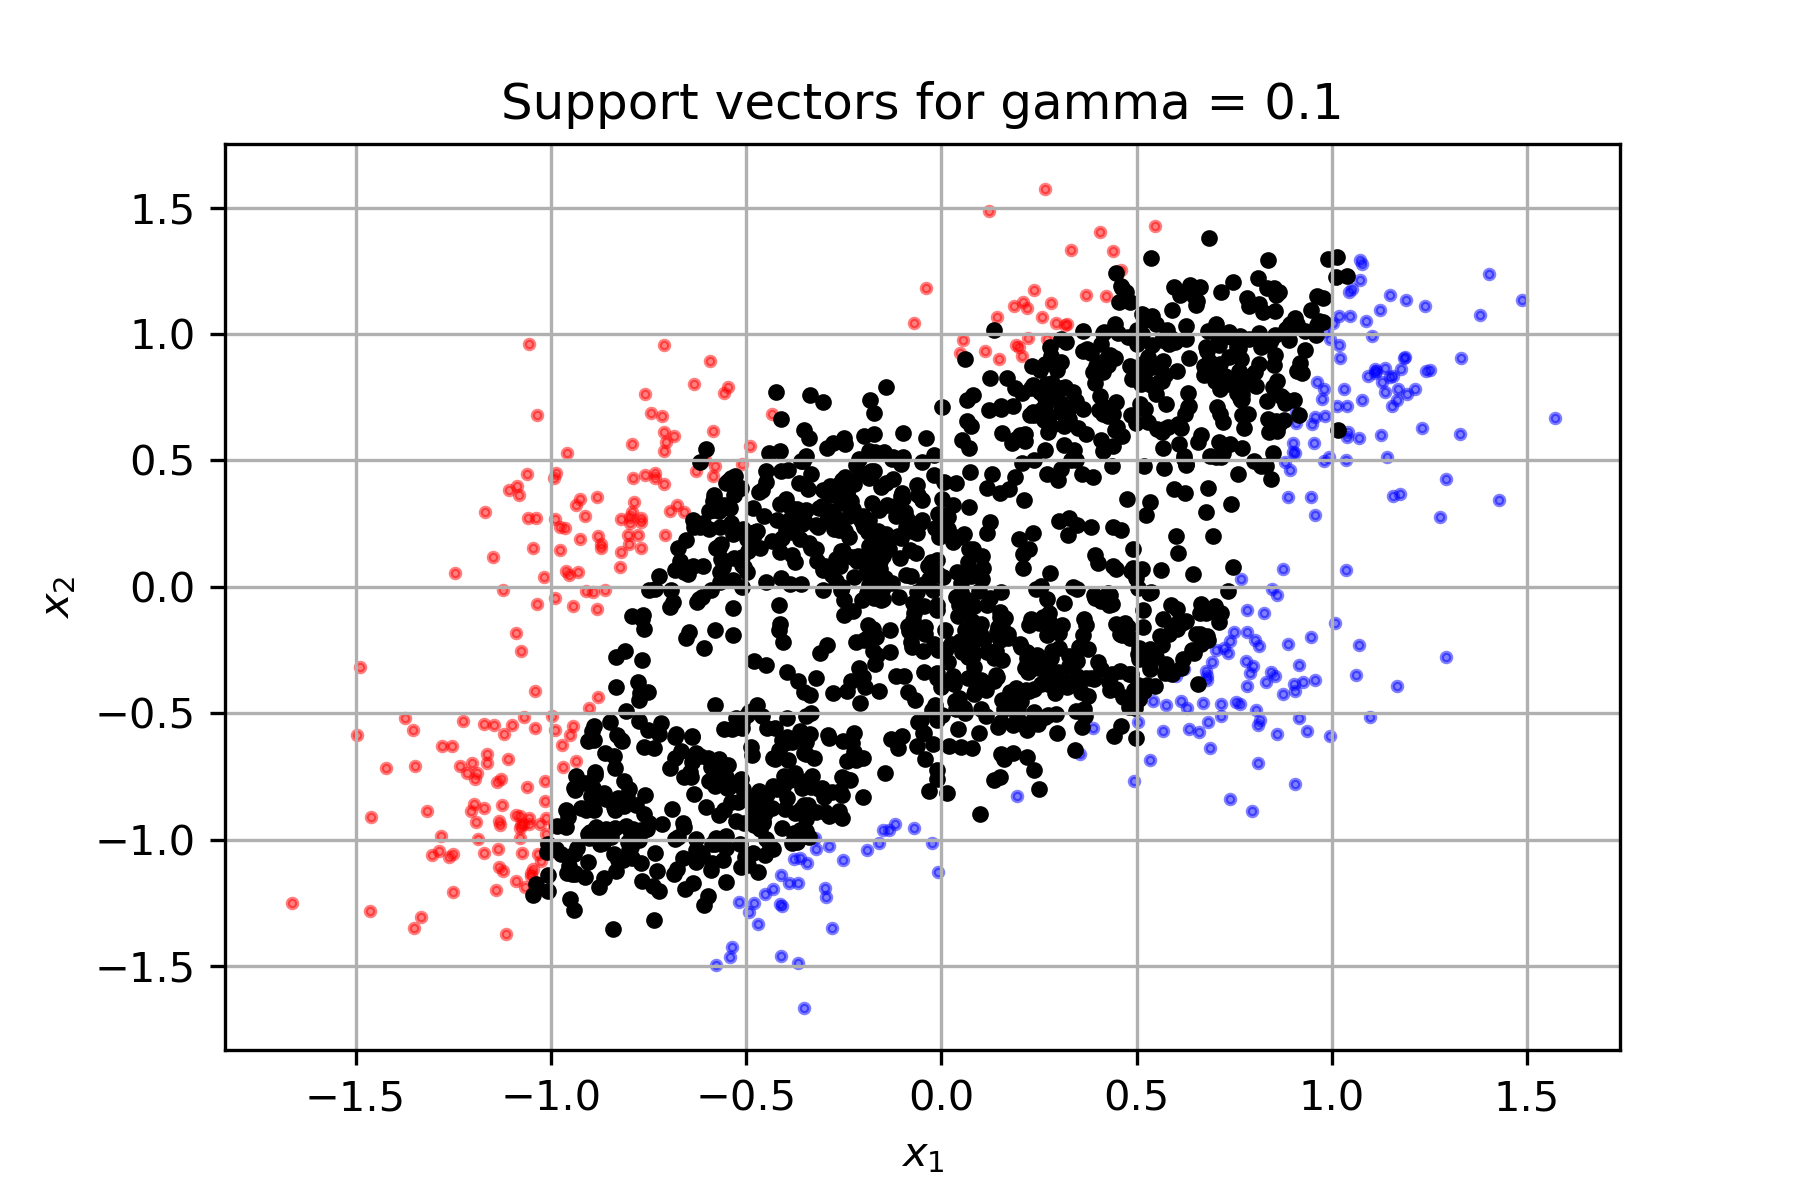
\includegraphics[width=7cm]{support_vectors_gamma_0d1}
        \caption{Support vectors for gamma = 0.1}
        \label{fig:svm-support_vectors_gamma_0d1}
    \end{subfigure}
    %-----------------------------------
    % decision regions (gamma = 1.0)
    \begin{subfigure}{0.45\textwidth}
        \centering
        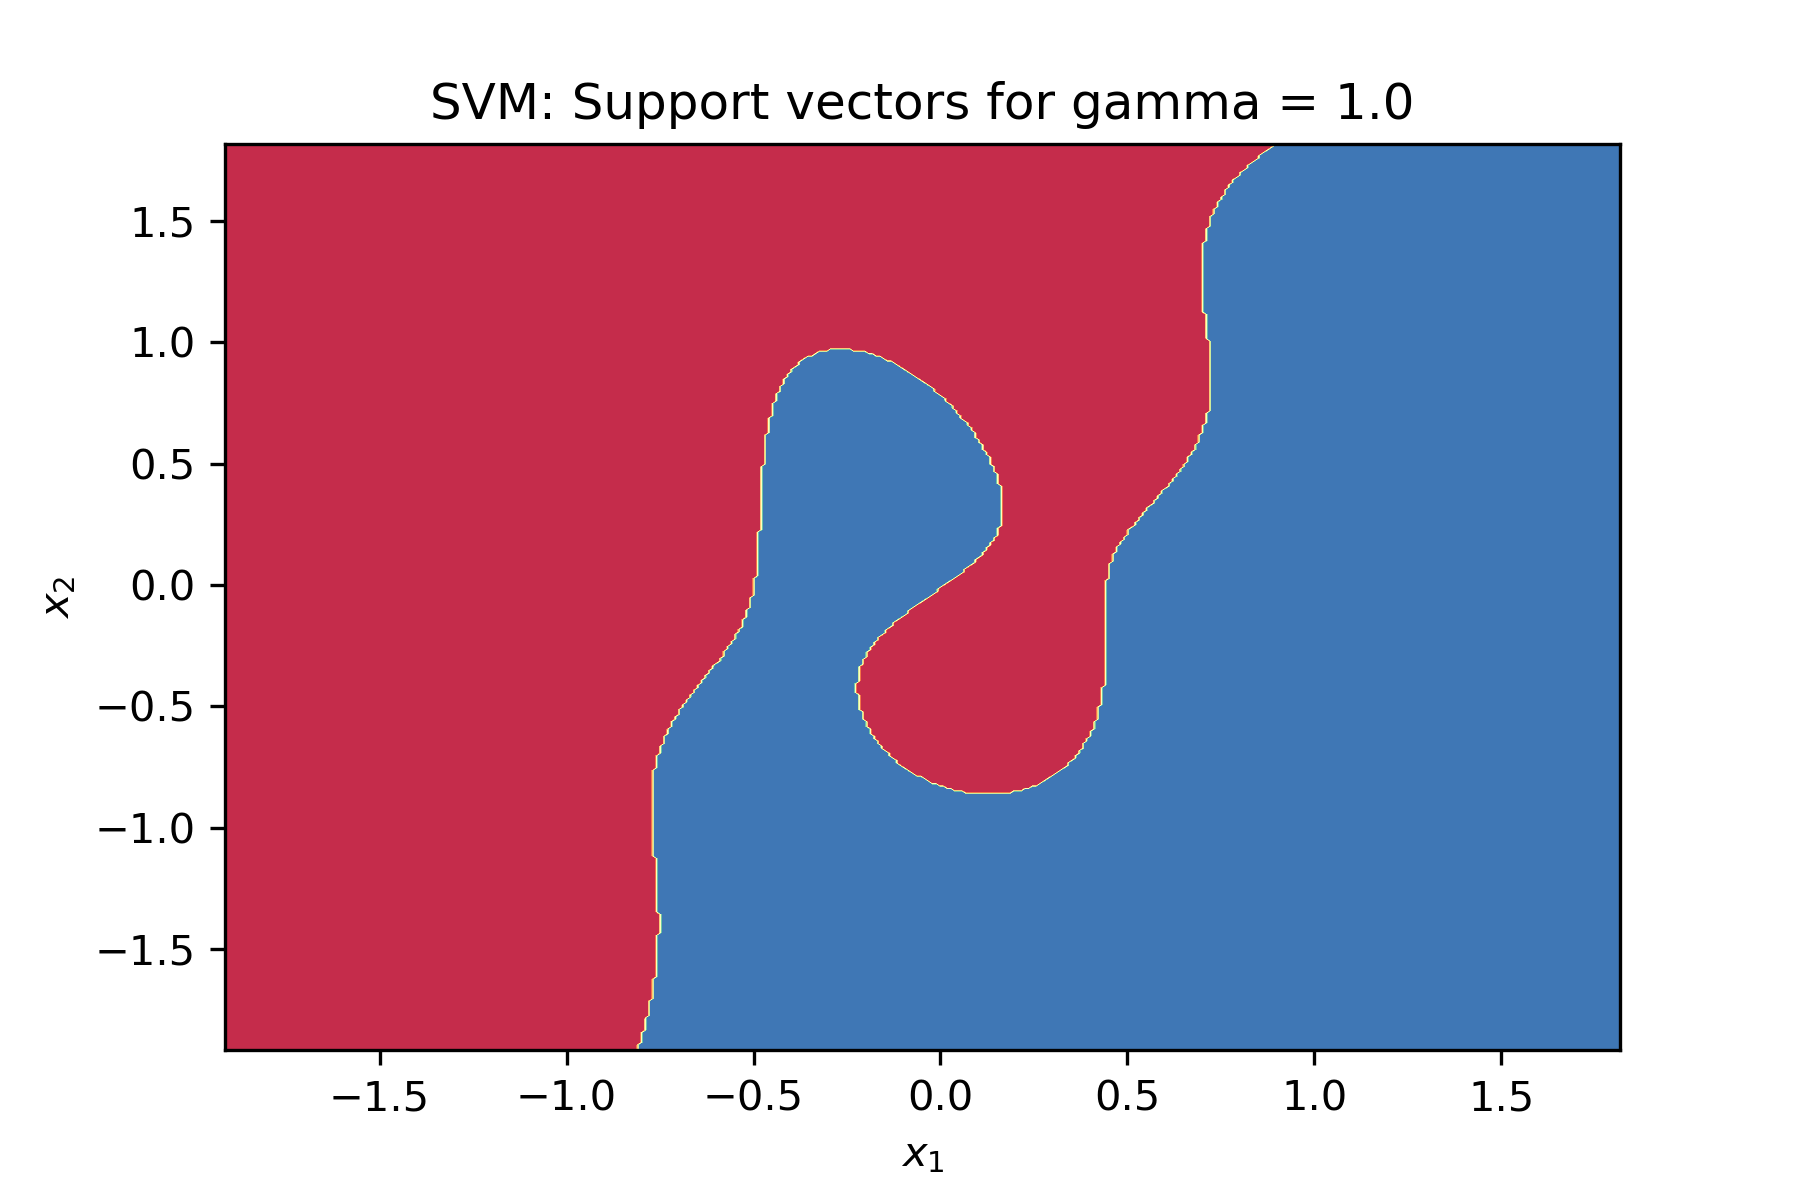
\includegraphics[width=7cm]{decision_region_gamma_1}
        \caption{Decision regions for gamma = 1.0}
        \label{fig:svm-decision_region_gamma_1}
    \end{subfigure}
    \hfill
    % support vectors (gamma = 1.0)
    \begin{subfigure}{0.45\textwidth}
        \centering
        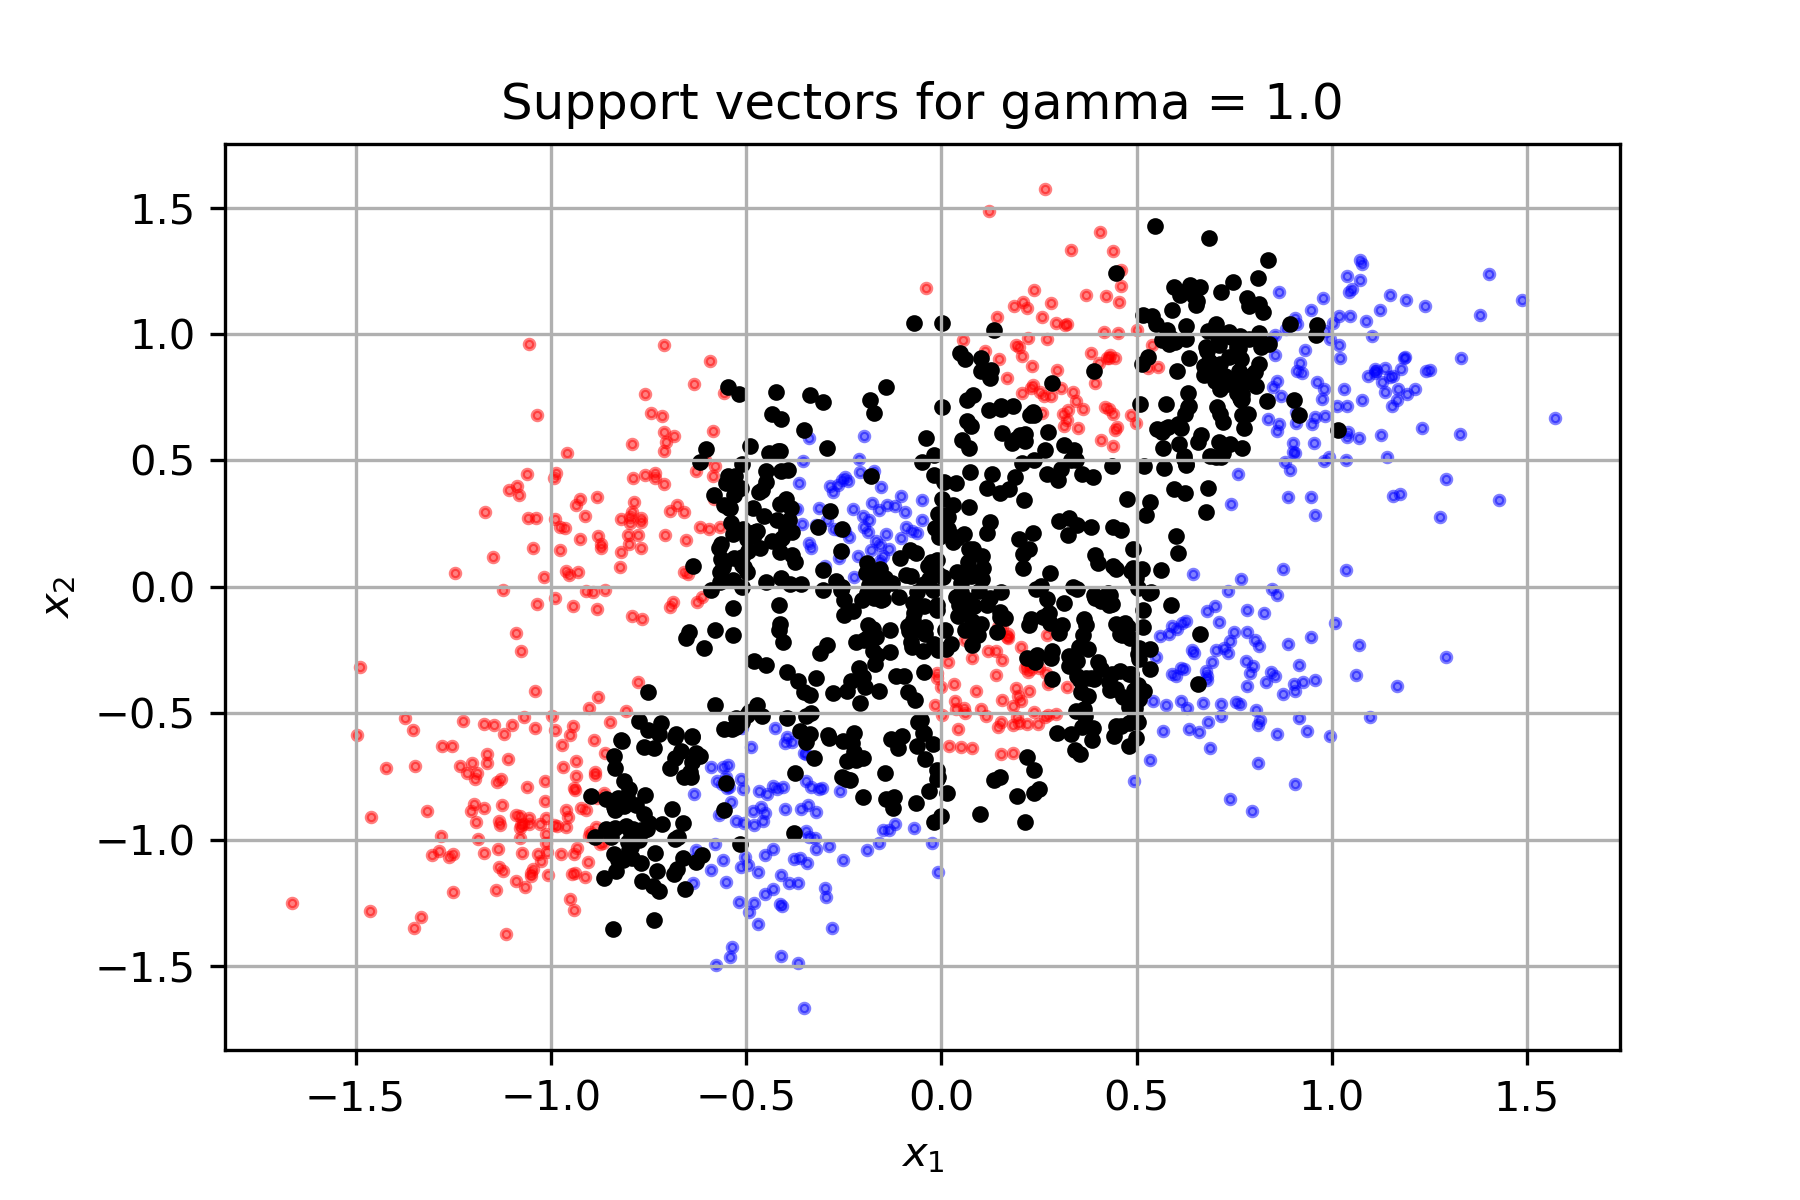
\includegraphics[width=7cm]{support_vectors_gamma_1}
        \caption{Support vectors for gamma = 1.0}
        \label{fig:svm-support_vectors_gamma_1}
    \end{subfigure}
    %-----------------------------------
    %% decision regions (gamma = 20)
    %\begin{subfigure}{0.45\textwidth}
    %    \centering
    %    \includegraphics[width=7cm]{decision_region_gamma_20}
    %    \caption{Decision regions for gamma = 20}
    %    \label{fig:svm-decision_region_gamma_20}
    %\end{subfigure}
    %\hfill
    %% support vectors (gamma = 20)
    %\begin{subfigure}{0.45\textwidth}
    %    \centering
    %    \includegraphics[width=7cm]{support_vectors_gamma_20}
    %    \caption{Support vectors for gamma = 20}
    %    \label{fig:svm-support_vectors_gamma_20}
    %\end{subfigure}
    %-----------------------------------
    % decision regions (gamma = 10)
    \begin{subfigure}{0.45\textwidth}
        \centering
        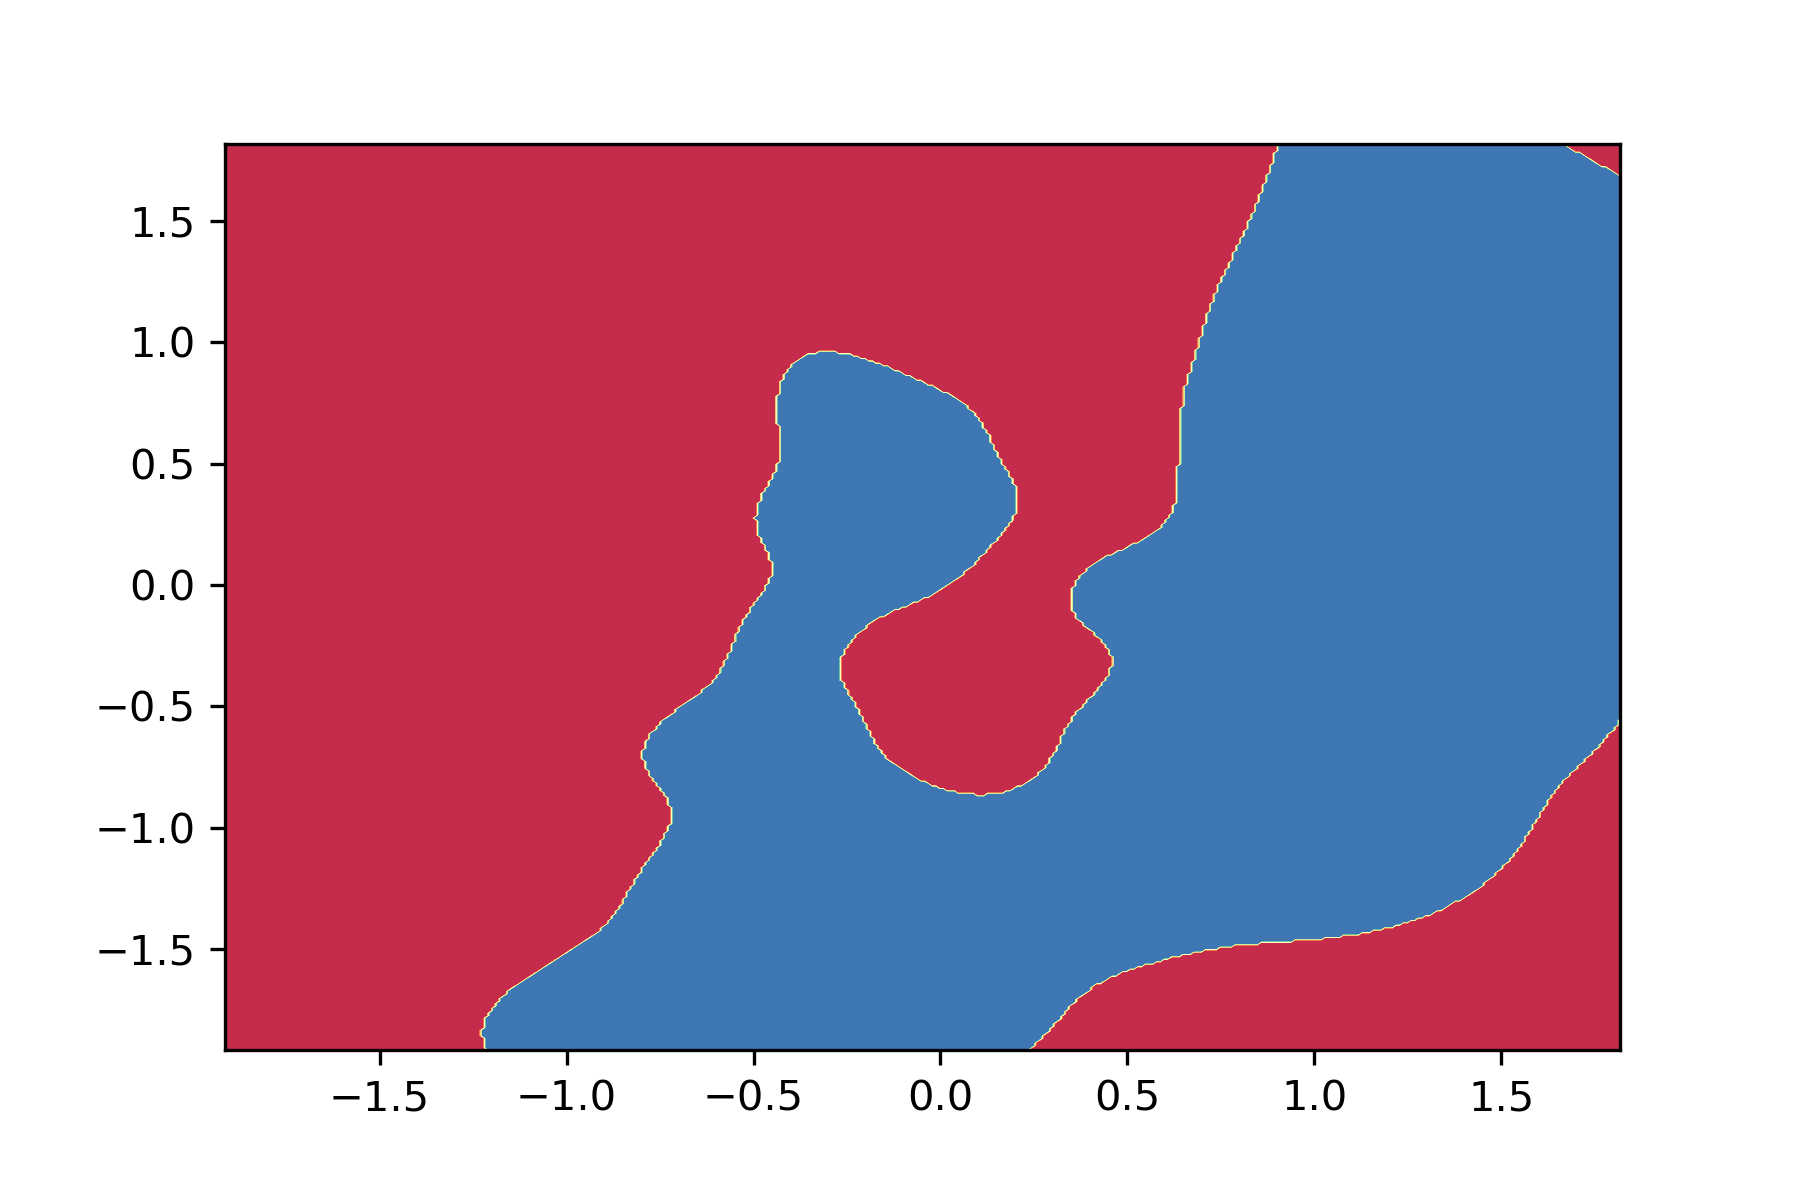
\includegraphics[width=7cm]{decision_region_gamma_10}
        \caption{Decision regions for gamma = 10}
        \label{fig:svm-decision_region_gamma_10}
    \end{subfigure}
    \hfill
    % support vectors (gamma = 10)
    \begin{subfigure}{0.45\textwidth}
        \centering
        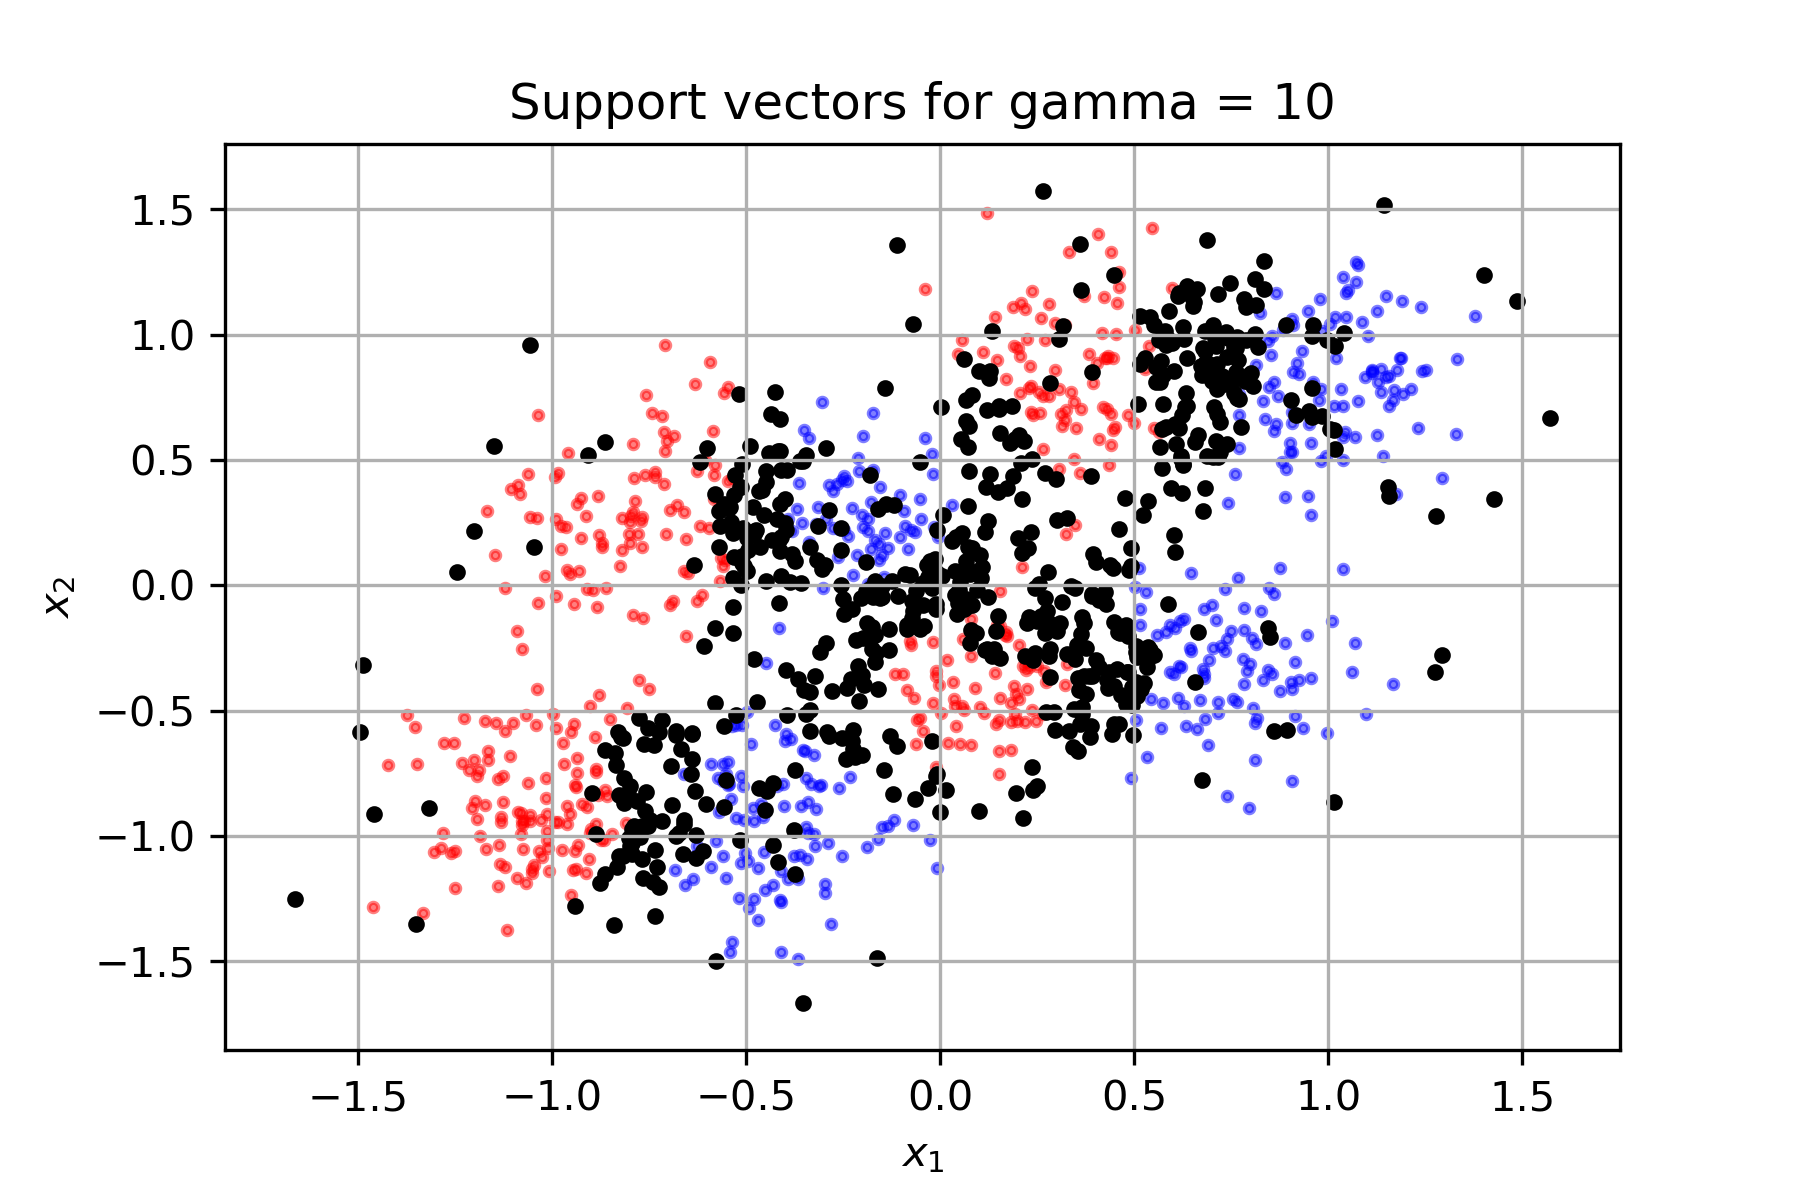
\includegraphics[width=7cm]{support_vectors_gamma_10}
        \caption{Support vectors for gamma = 10}
        \label{fig:svm-support_vectors_gamma_10}
    \end{subfigure}
    %-----------------------------------
    % caption and label
    \caption{Decision regions and respective support vectors for different values of hyperparameter gamma in kernel function}
    \label{fig:svm-decision_regions_support_vectos_gamma}
\end{figure}
%-------------------------------------------------


%=================================================
\end{document}
